\section{Intergenic regions}

Fourteen datasets from various tissues (blood, brain, eye, and lung) were analyzed.
These datasets contained between 11\% and 29\% unassigned uniquely mapped reads (as shown in Table \ref{tab:countStats})
when using the 10x reference.
Additionally, 6\% to 18\% of total reads were intergenic, meaning they did not overlap with any reference used.
Given the size of the datasets, such a proportion of reads could potentially contain biologically relevant information.

??????????????????????????????????????????

Also, one can observe that the proportions of unassigned and intergenic reads are higher when samples are first demultiplexed by UMIs.
This suggests that unassigned transcripts are present in lower amounts than assigned ones.
If all unassigned transcripts originated from unannotated genes,
one would expect amplification to occur similarly for both assigned and unassigned transcripts.
However, this is not the case, which suggests that additional factors contribute to the discrepancy.
One possible explanation is polymerase error, particularly template switching.

\textcite{Kebschull2015} demonstrated that template switching occurs during PCR amplification, albeit rarely.
Notably, these events are more common in the later cycles of PCR (\cite{Kebschull2015}),
meaning that the resulting chimeric transcripts undergo fewer amplification cycles and thus appear at lower abundances in the data.
While this could partially account for the reduced amplification of unassigned transcripts, it is unlikely to be the sole explanation.

?????????????????????????????



\begin{table}[h]
    \centering
    \resizebox{\textwidth}{!}{
    \begin{tabular}{l|rrr|rrr}
    \toprule
    Sample & Total Reads & Unassigned & Intergenic & Demultiplexed & Unassigned & Intergenic \\
    \midrule
    PBMC\_10x & 182330834 & 15.95\% & 11.37\% & 70305137 & 18.51\% & 12.86\% \\
    PBMC\_10x\_2 & 496387931 & 18.52\% & 14.26\% & 195948926 & 21.29\% & 16.32\% \\
    PBMC\_10x\_3 & 368640939 & 18.59\% & 14.34\% & 167804193 & 20.99\% & 16.17\% \\
    PBMC\_indrops & 112932507 & 11.12\% & 6.5\% & 8176578 & 22.86\% & 10.25\% \\
    PBMC\_indrops\_2 & 471705924 & 14.87\% & 8.36\% & 98063027 & 25.52\% & 13.73\% \\
    brain & 206360627 & 16.87\% & 10.67\% & 143916177 & 19.02\% & 12.07\% \\
    brain\_2 & 122556503 & 22.32\% & 15.98\% & 95031864 & 23.77\% & 17.00\% \\
    eye & 375397270 & 28.02\% & 18.97\% & 161882445 & 31.87\% & 21.60\% \\
    eye\_2 & 140981808 & 29.35\% & 14.85\% & 69146995 & 31.43\% & 15.99\% \\
    eye\_3 & 161261977 & 29.46\% & 18.86\% & 68157696 & 32.11\% & 20.58\% \\
    lung\_2 & 511080104 & 15.99\% & 12.07\% & 269118747 & 17.98\% & 13.33\% \\
    lung\_5 & 452105505 & 14.49\% & 10.74\% & 256353198 & 16.19\% & 11.83\% \\
    lung\_7 & 524095146 & 18.41\% & 14.34\% & 236157103 & 20.64\% & 15.79\% \\
    lung\_8 & 342092138 & 14.53\% & 10.66\% & 217801055 & 16.07\% & 11.67\% \\
    \bottomrule
    \end{tabular}
    }
    \caption{Statistics of unassigned and intergenic reads per sample.
    Unassigned reads were counted after mapping with 10x reference.
    Intergenic reads here are those that do not intersect with any reference used.
    'Demultiplexed' column shows number of total reads after demultiplexing using UMIs,
    and following 'unassigned' and 'intergenic' percentages were computed compared to this number.}
    \label{tab:countStats}
\end{table}

\paragraph{Analysing integenic regions}

For each sample, intergenic regions containing a sufficient number of unassigned reads were identified,
as described in the methods section (with a threshold set at 5 CPM).
The term "intergenic" is used here in a strand-specific manner,
meaning an "intergenic" region may be located on the opposite strand of a known gene.

To determine whether these intergenic regions contain biologically meaningful information,
cells in each sample were clustered based solely on reads from these regions.
As shown in selected examples in Figure \ref{fig:intergenicClustering},
clustering was observed and roughly corresponded to clustering based on the standard ("10x") annotation.
This indicates that biologically meaningful information is indeed present in these intergenic regions.
Consequently, further analyses were performed on these regions.

The lists of intergenic regions from all samples were combined and filtered based on the number of samples in which they were detected,
resulting in a final set of 2,590 intergenic regions.
Of these, 147 did not overlap known genes on the opposite strand and will be referred to as "isolated".
Those located on the opposite strand of known genes will be referred to as "antisense".

\begin{figure}[htbp]
    \centering
    \begin{subfigure}{0.45\textwidth}
        \centering
        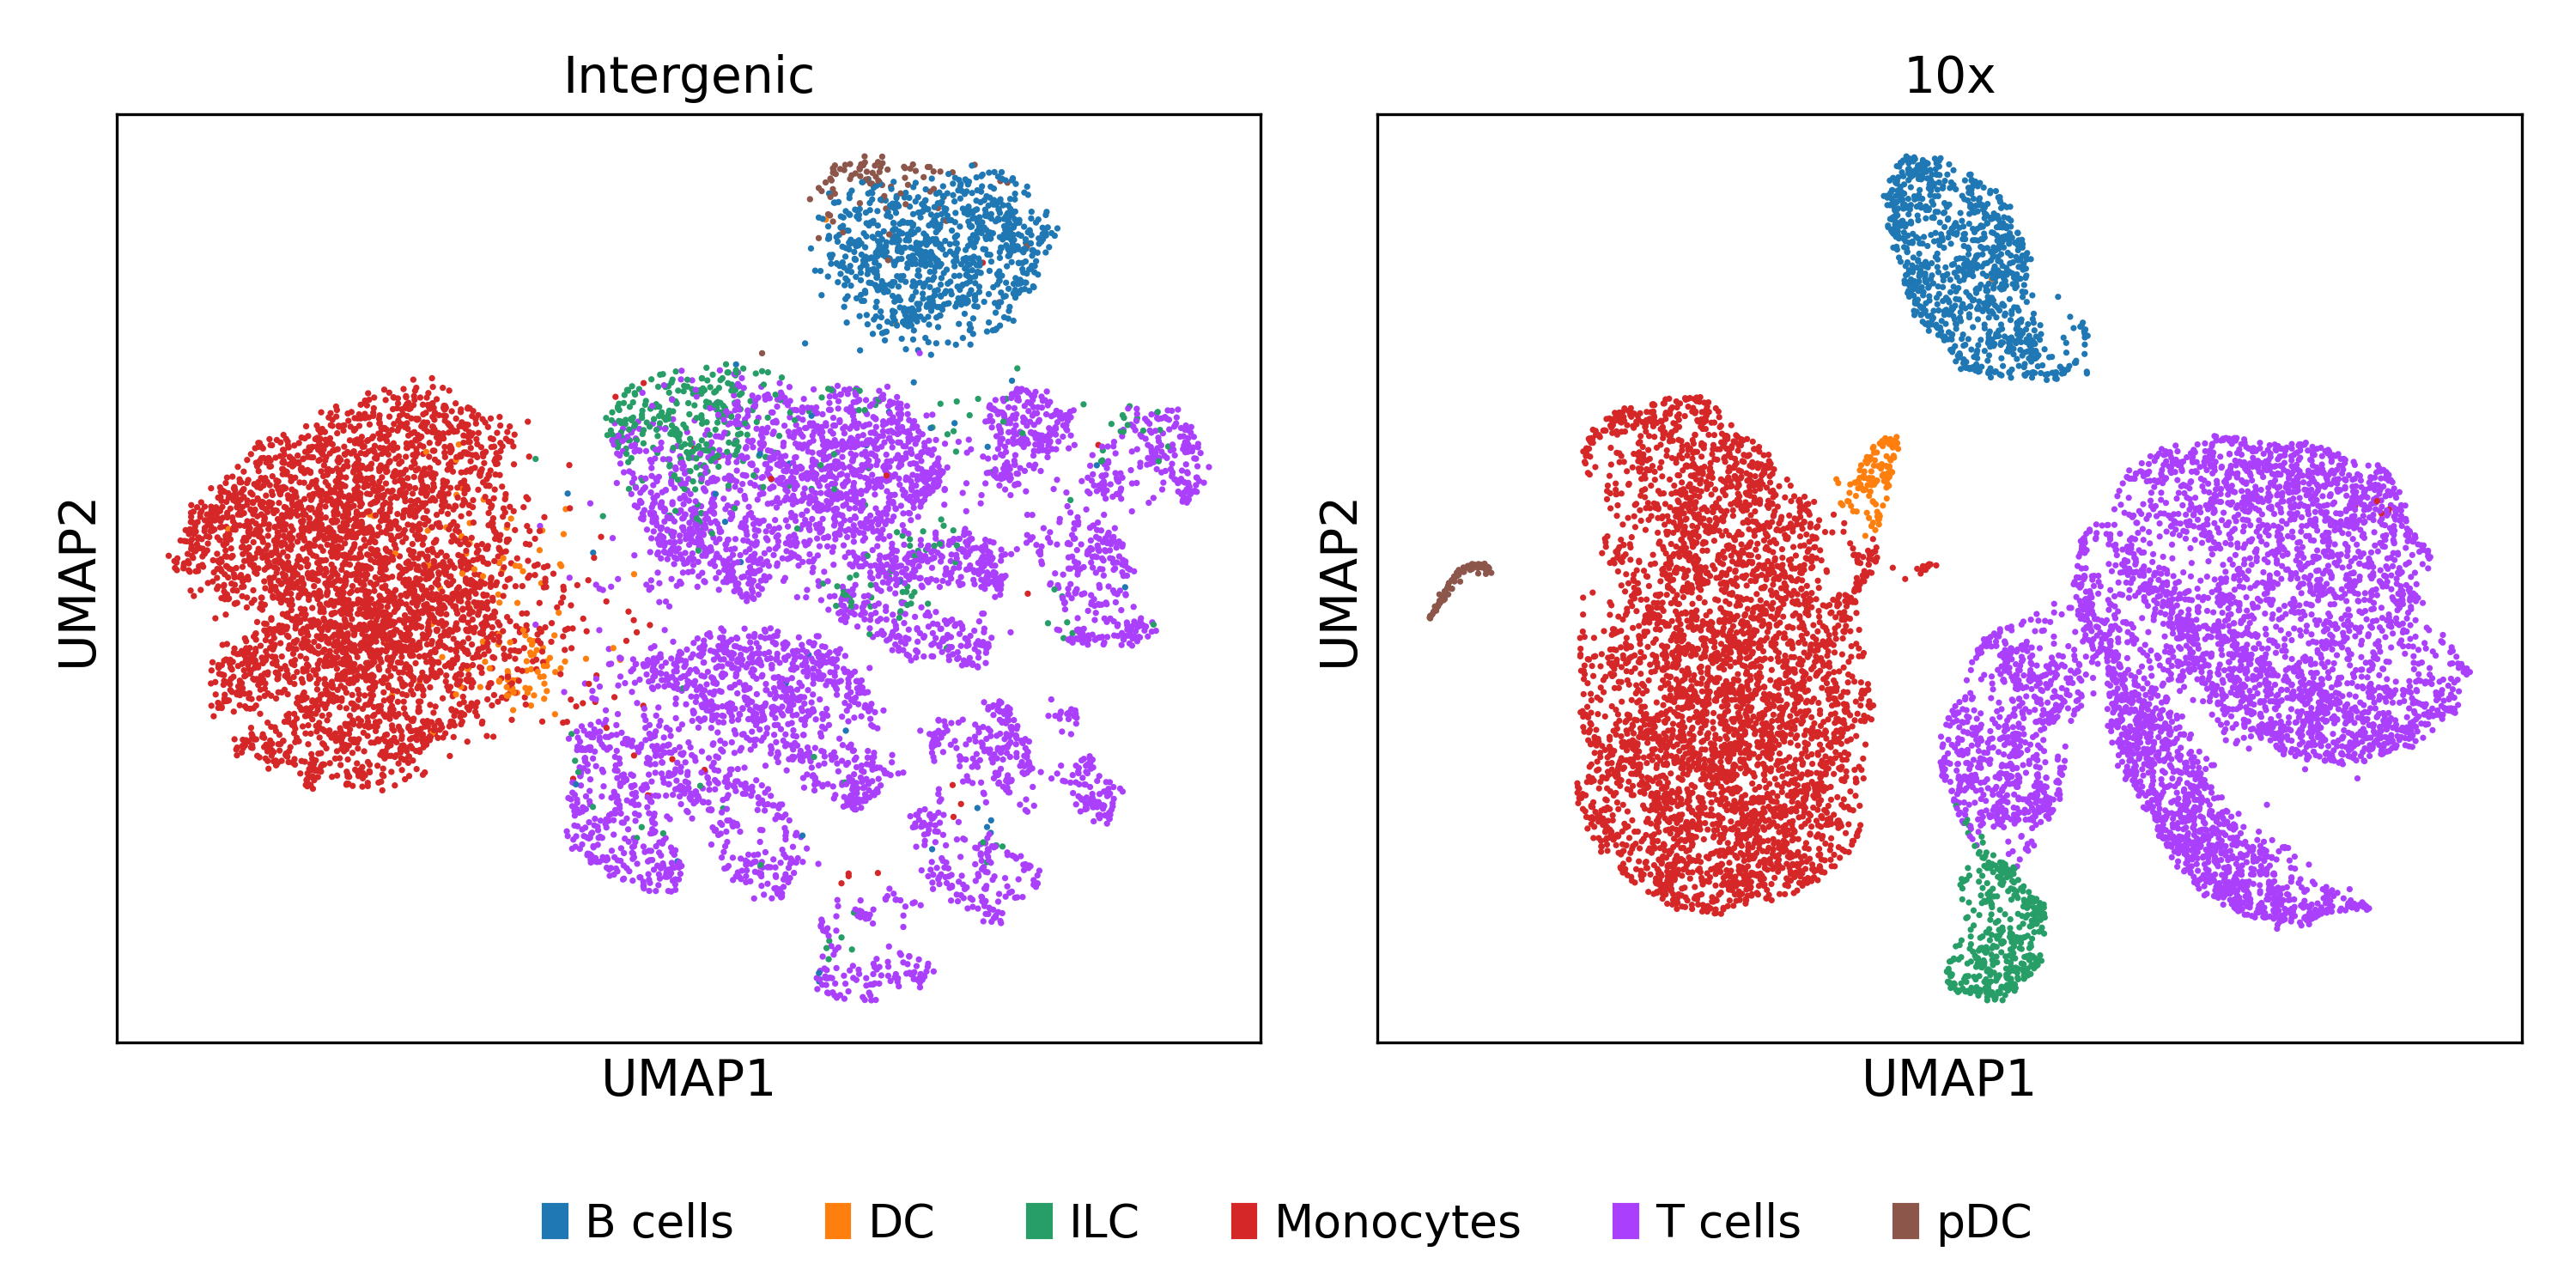
\includegraphics[width=\textwidth]{images/umaps/intergenic_10x_pbmc10x3.png}
        \caption{10x PBMC 3}
    \end{subfigure}
    \hfill
    \begin{subfigure}{0.45\textwidth}
        \centering
        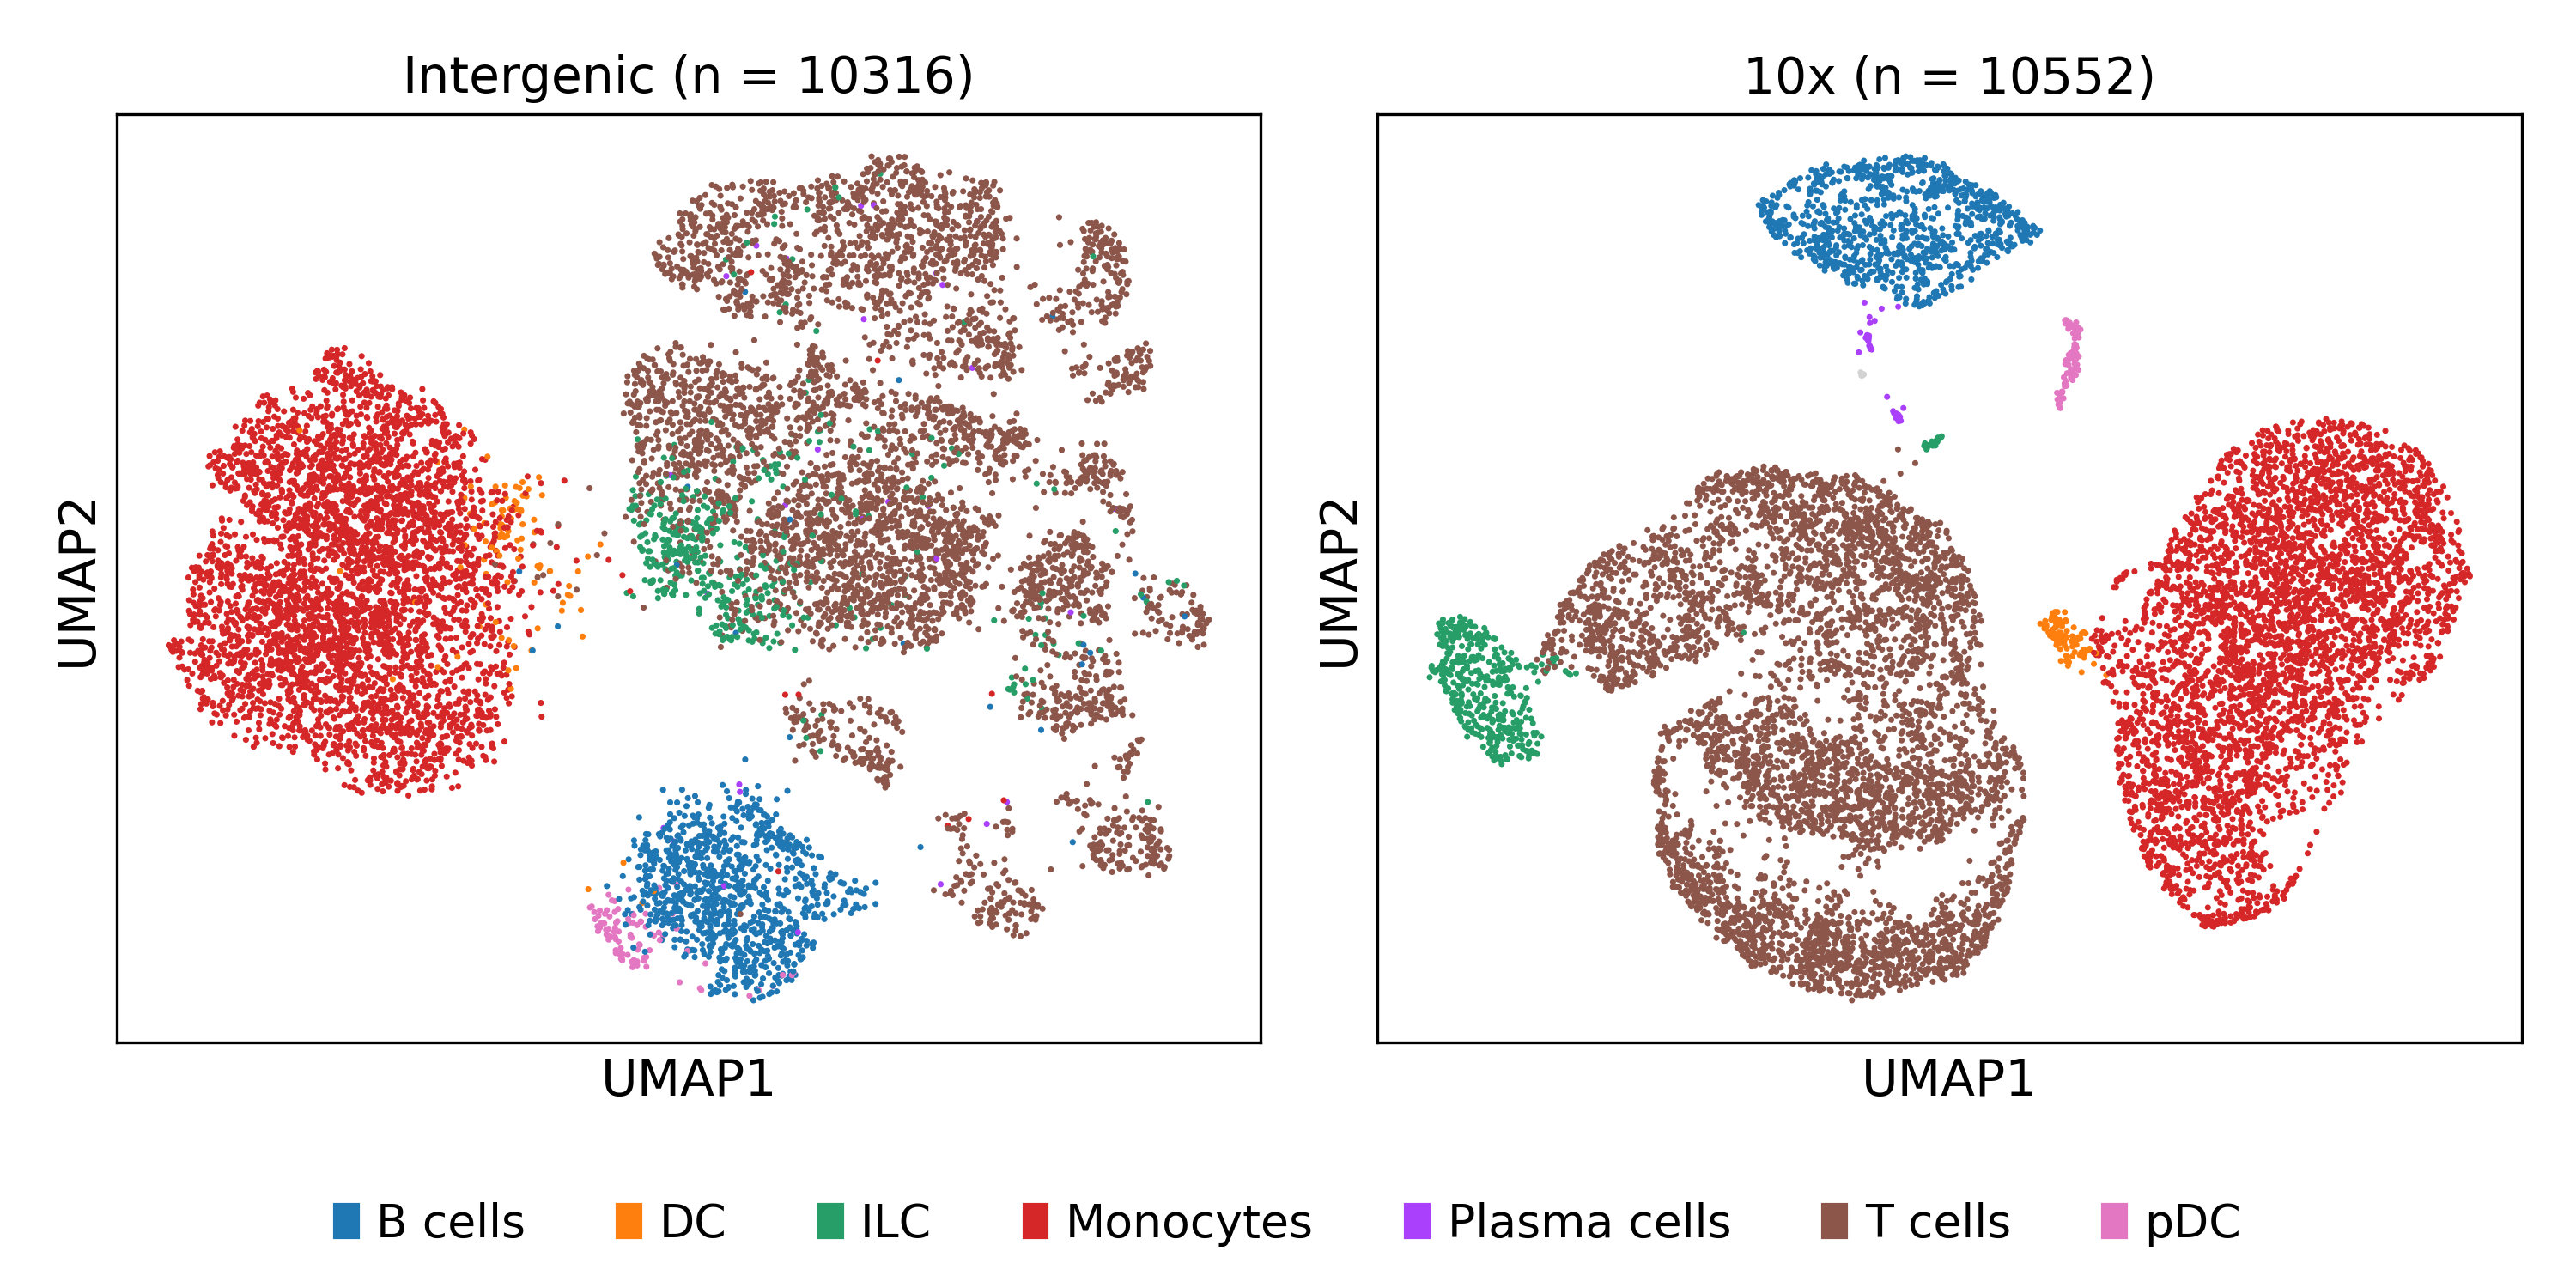
\includegraphics[width=\textwidth]{images/umaps/intergenic_10x_pbmc10x2.png}
        \caption{10x PBMC 2}
    \end{subfigure}
    \vspace{0.5em}
    \begin{subfigure}{0.45\textwidth}
        \centering
        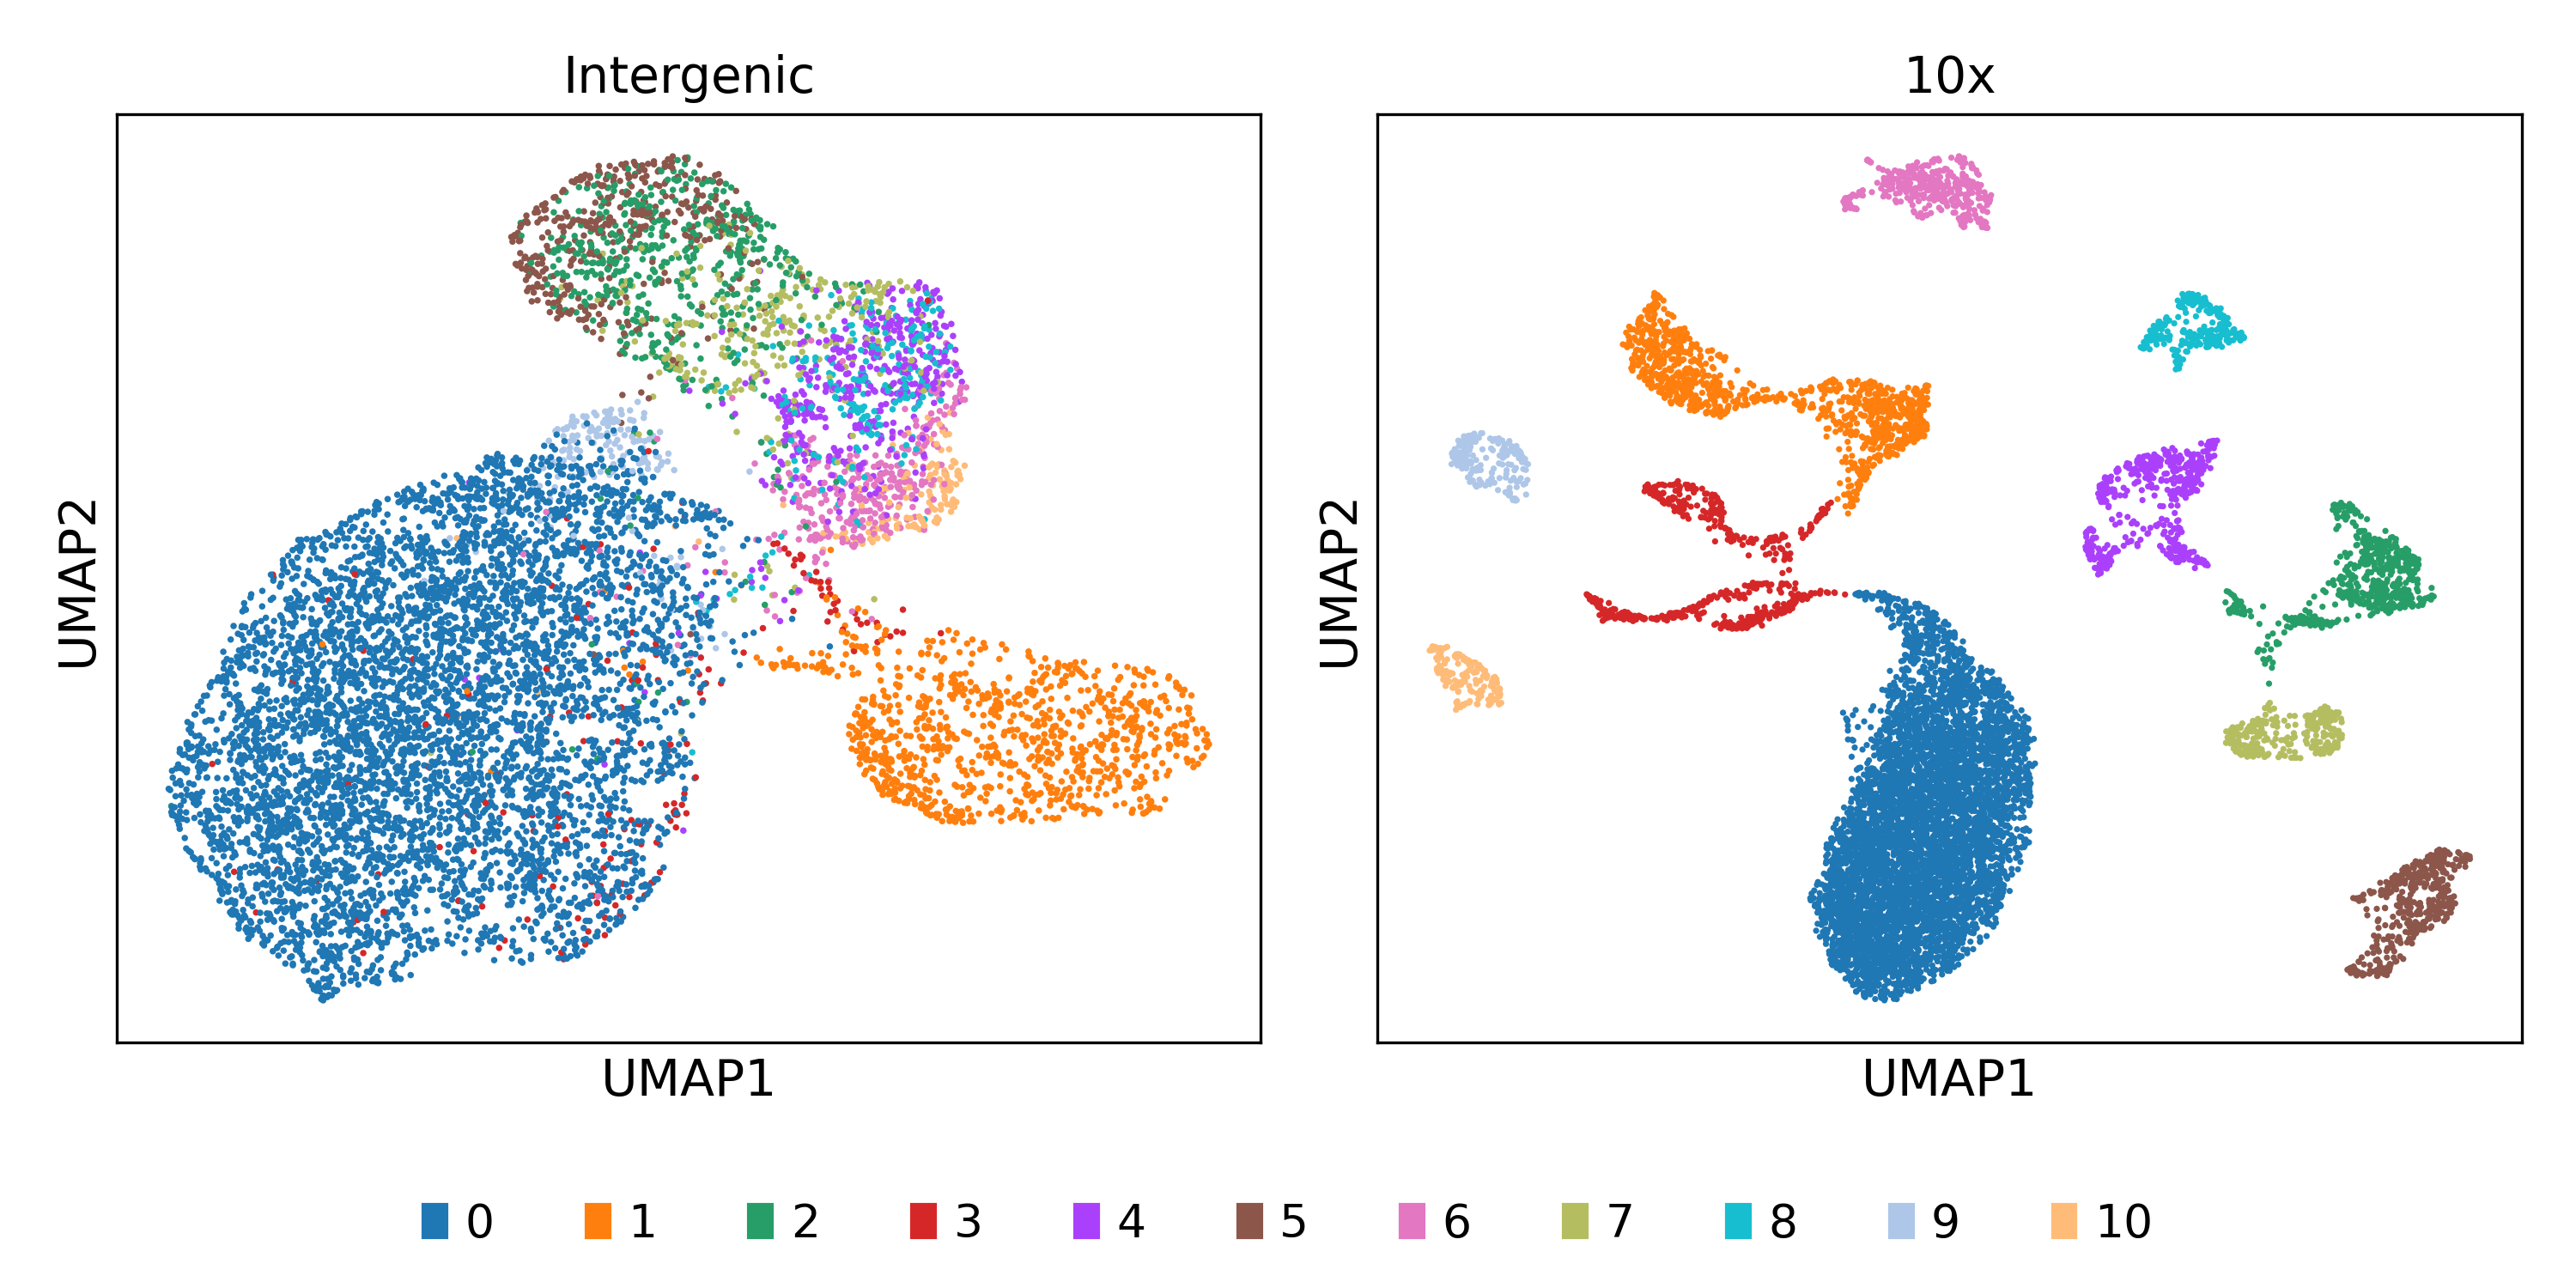
\includegraphics[width=\textwidth]{images/umaps/intergenic_10x_eye.png}
        \caption{eye}
    \end{subfigure}
    \hfill
    \begin{subfigure}{0.45\textwidth}
        \centering
        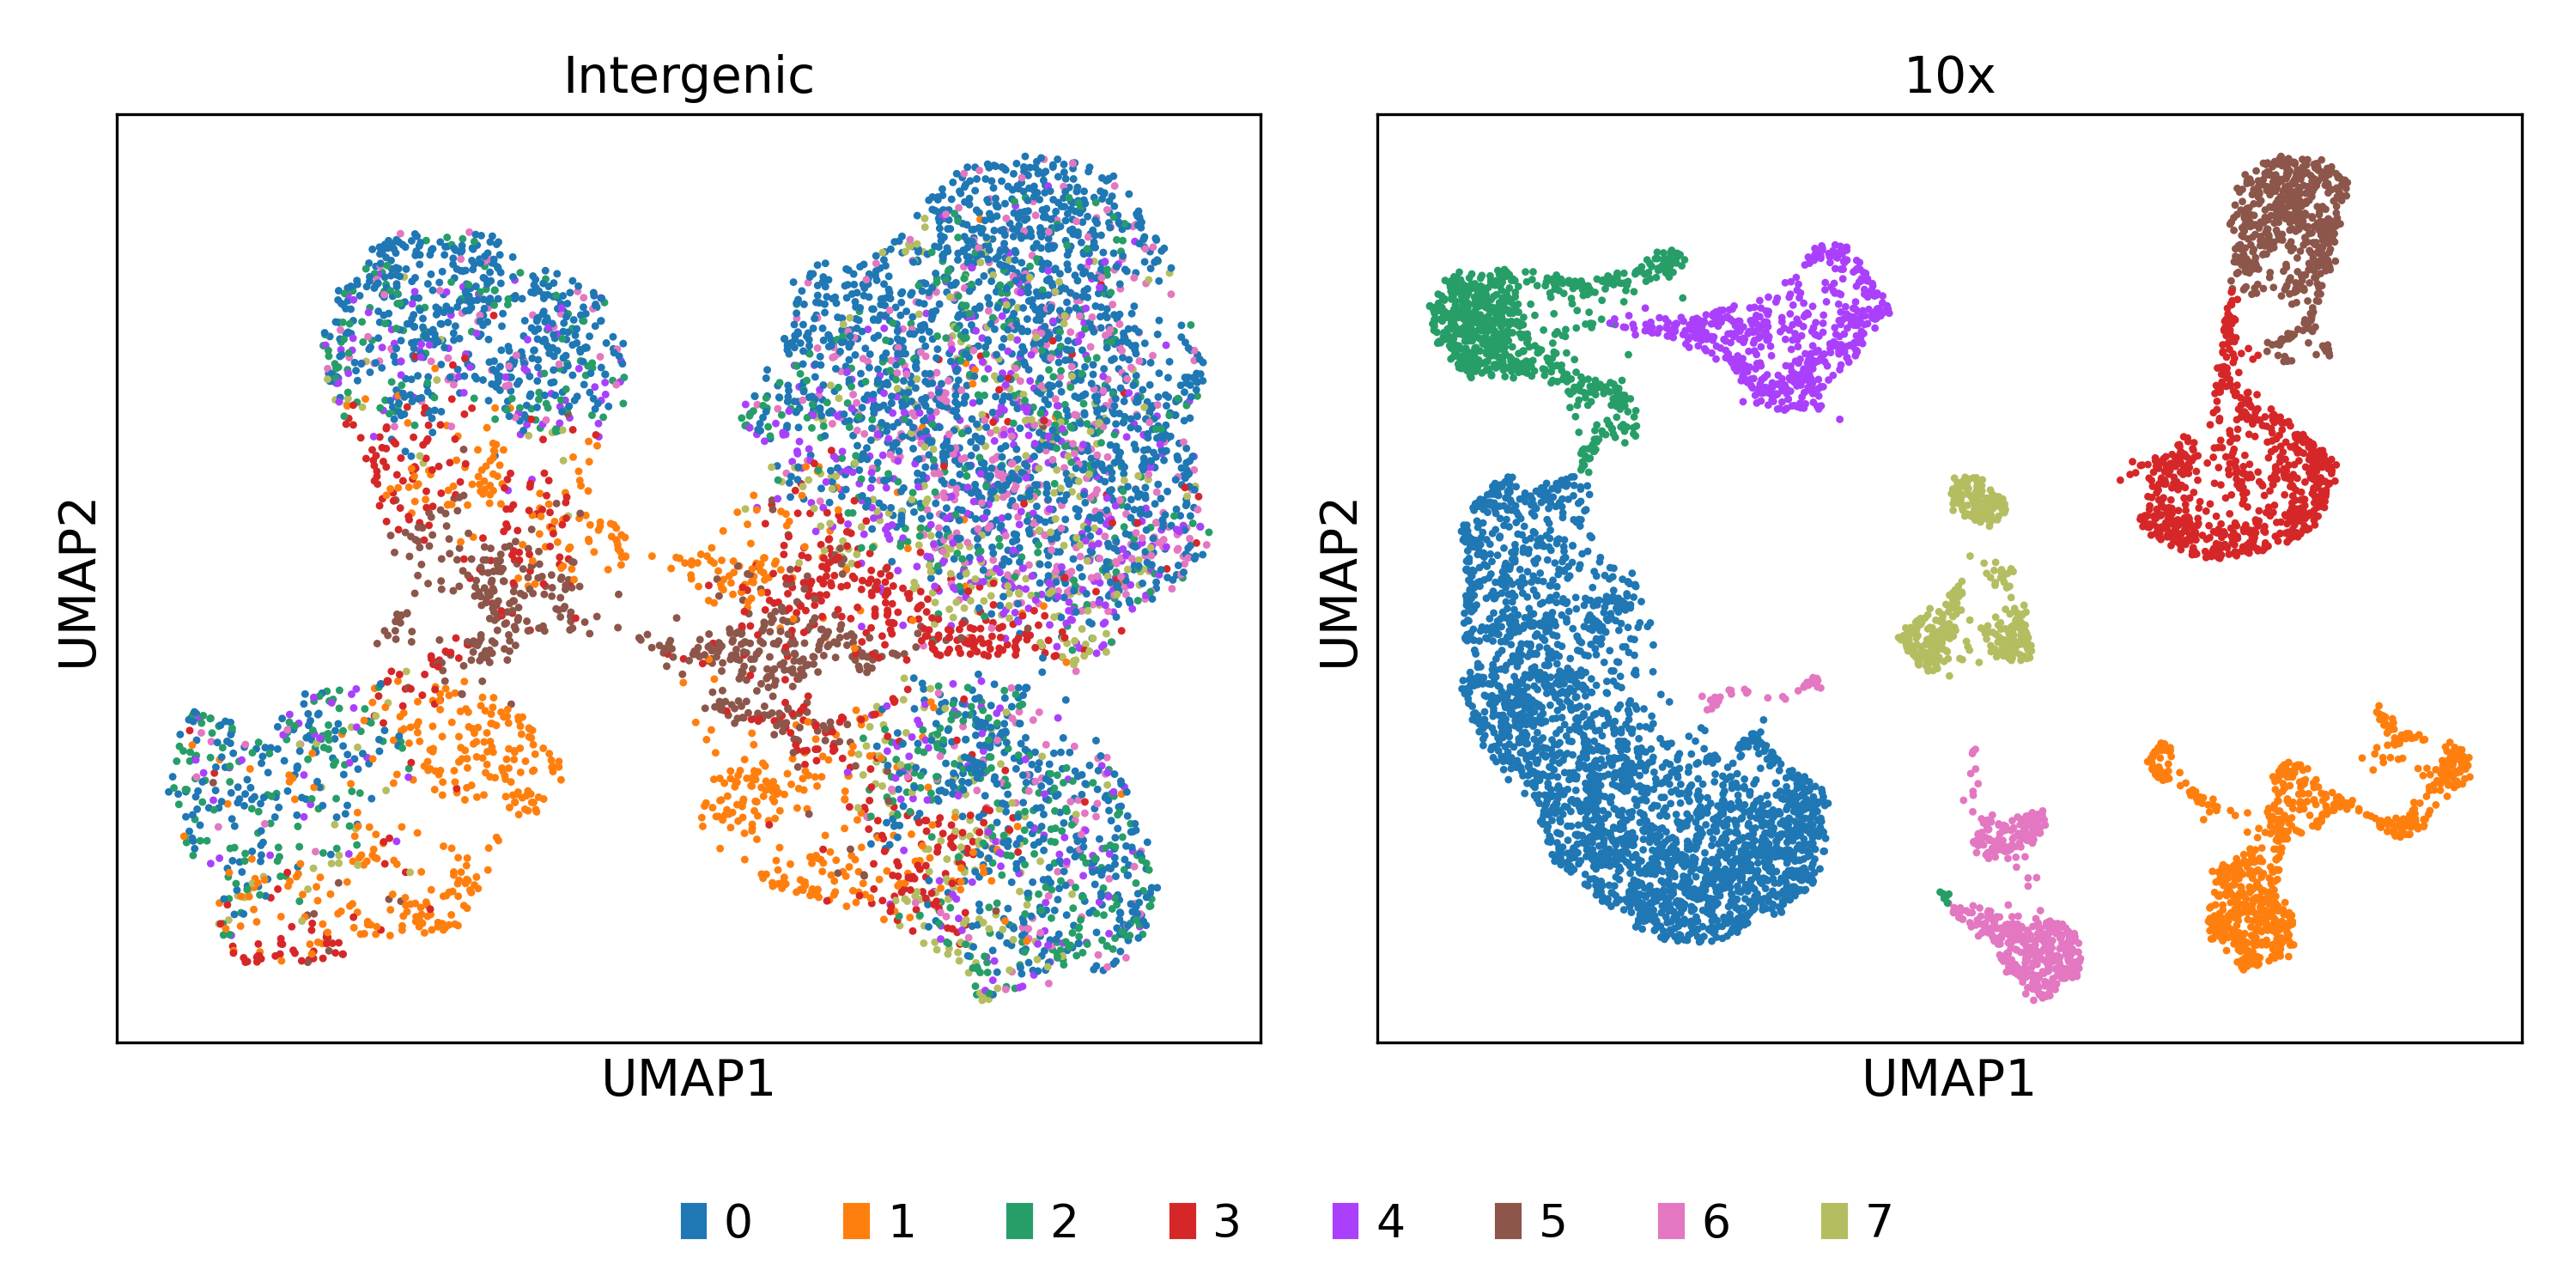
\includegraphics[width=\textwidth]{images/umaps/intergenic_10x_brain_2.png}
        \caption{10x Brain 2}
    \end{subfigure}
    \caption{Comparison of clustering using standard annotation ('10x' reference) and using only defined intergenic regions.
    As can be seen, for some samples intergenic regions are sufficient for rough clustering, for others (e.g. 'brain\_2' sample), 
    noise gives some clustering artefacts.
    Nevertheless, this rough clustering implies that these unassigned read contain biological information.}
    \label{fig:intergenicClustering}
\end{figure}

\paragraph{A-rich sequences near the intergenic regions 3' end}

If there is poly-A region near the 3' end of the intergenic region, then the presence of those peaks can be explained by mis-priming,
i.e. that would suggest that our intergenic region is not necessarily the actual 3' end of the novel transcript, but may be in the middle of it.

This is indeed the case for the most of reported intergenic regions,
see Figure \ref{fig:polyAdistances} for histogram and Table \ref{tab:polyAstats} for some statistics.

\begin{figure}
  \centering
  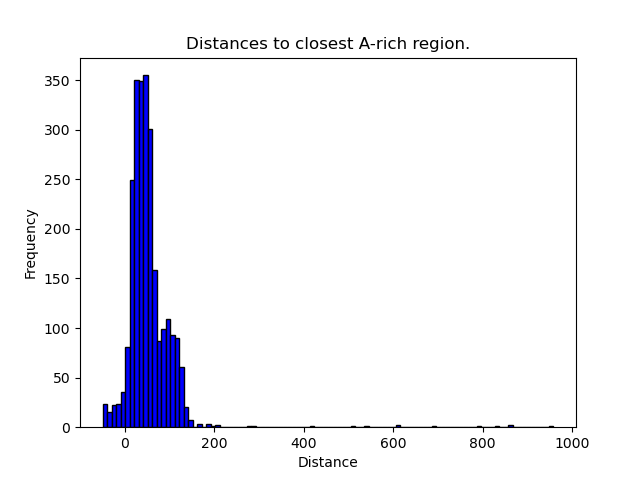
\includegraphics[width=0.5\linewidth]{images/poly-A-distances.png}
  \caption{Distances from 3' ends to closest A-rich region downstream.
  From all the intergenic regions, only 40 do not have such region within 1kb from the 3' end.}
  \label{fig:polyAdistances}
\end{figure}

\begin{table}[htbp]
  \centering
  \begin{tabular}{l|ccc}
    \toprule
     & isolated & antisense & total  \\
    \midrule
    mean distance & 54.8768 & 52.3499 & 52.4867 \\
    mean A-rich region length & 14.8333 & 16.755 & 16.651 \\
    \bottomrule
  \end{tabular}
  \caption{Summary of stats.}
  \label{tab:polyAstats}
\end{table}


\paragraph{Correlations}

Another aspect to check is whether expression of those intergenic regions correlate with the expression of nearby genes.
If it does, it might indicate several things:
\begin{itemize}
  \item If the region correlates with gene on the same strand:
  \begin{itemize}
    \item There might exist longer unannotated transcripts that involve those intergenic regions.
    \item The intergenic genes are involved in the same processes as the gene.
    \item They both can be transcribed by the same polymerases.
  \end{itemize}
  \item If the region correlates with gene on the oposite strand:
  \begin{itemize}
    \item The intergenic gene is involved in the same processes as the gene on the oposite strand.
    \item There happens some transcription errors that cause transcription from the opposite strand.
    \item There happens some errors in the library preparation/sequencing steps that cause template switch.
  \end{itemize}
\end{itemize}

Which of those are the case in our samples, is hard to tell.
Out of all defined intergenic regions, 86 showed Spearman correlation \textgreater 0.5 (p \textless 0.05) in at least 1 sample
(80 correlated with genes on the opposite strand, 10 with gene on the same strand, 4 with both).
Some examples can be seen in Figure \ref{fig:correlationUmaps}.

\begin{figure}[htbp]
    \centering
    \begin{subfigure}{\textwidth}
        \centering
        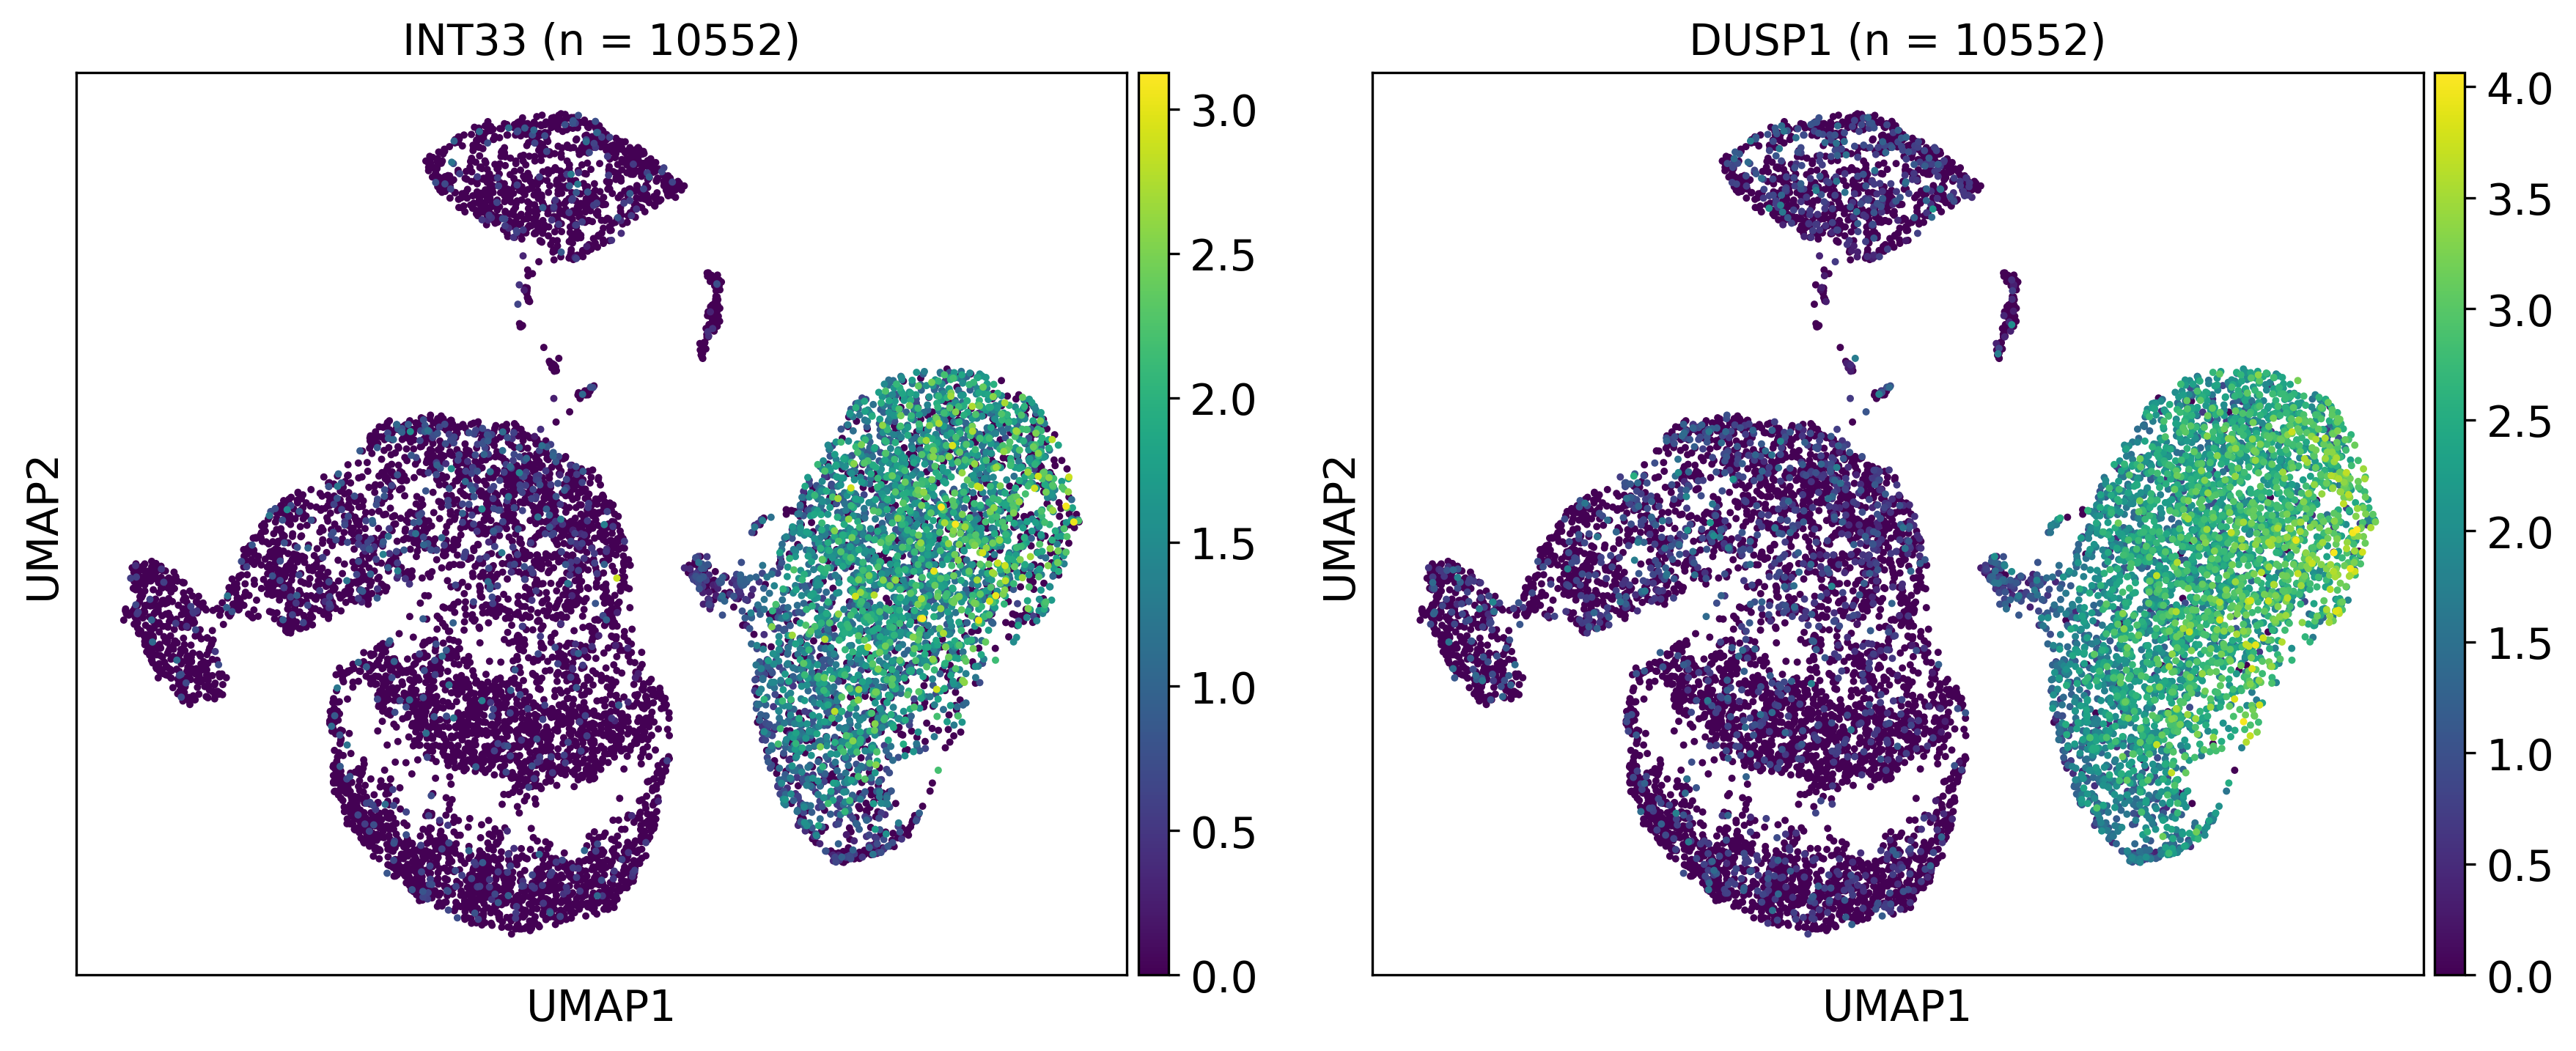
\includegraphics[width=\textwidth]{images/correlationUmaps/PBMC_10x_2_DUSP1.png}
        \caption{Umaps of INT33 and DUSP1 (Spearman correlation 0.68) of the PBMC\_10x\_2 sample, both of them are on the same strand.}
    \end{subfigure}
    \vspace{0.5em}
    \begin{subfigure}{\textwidth}
        \centering
        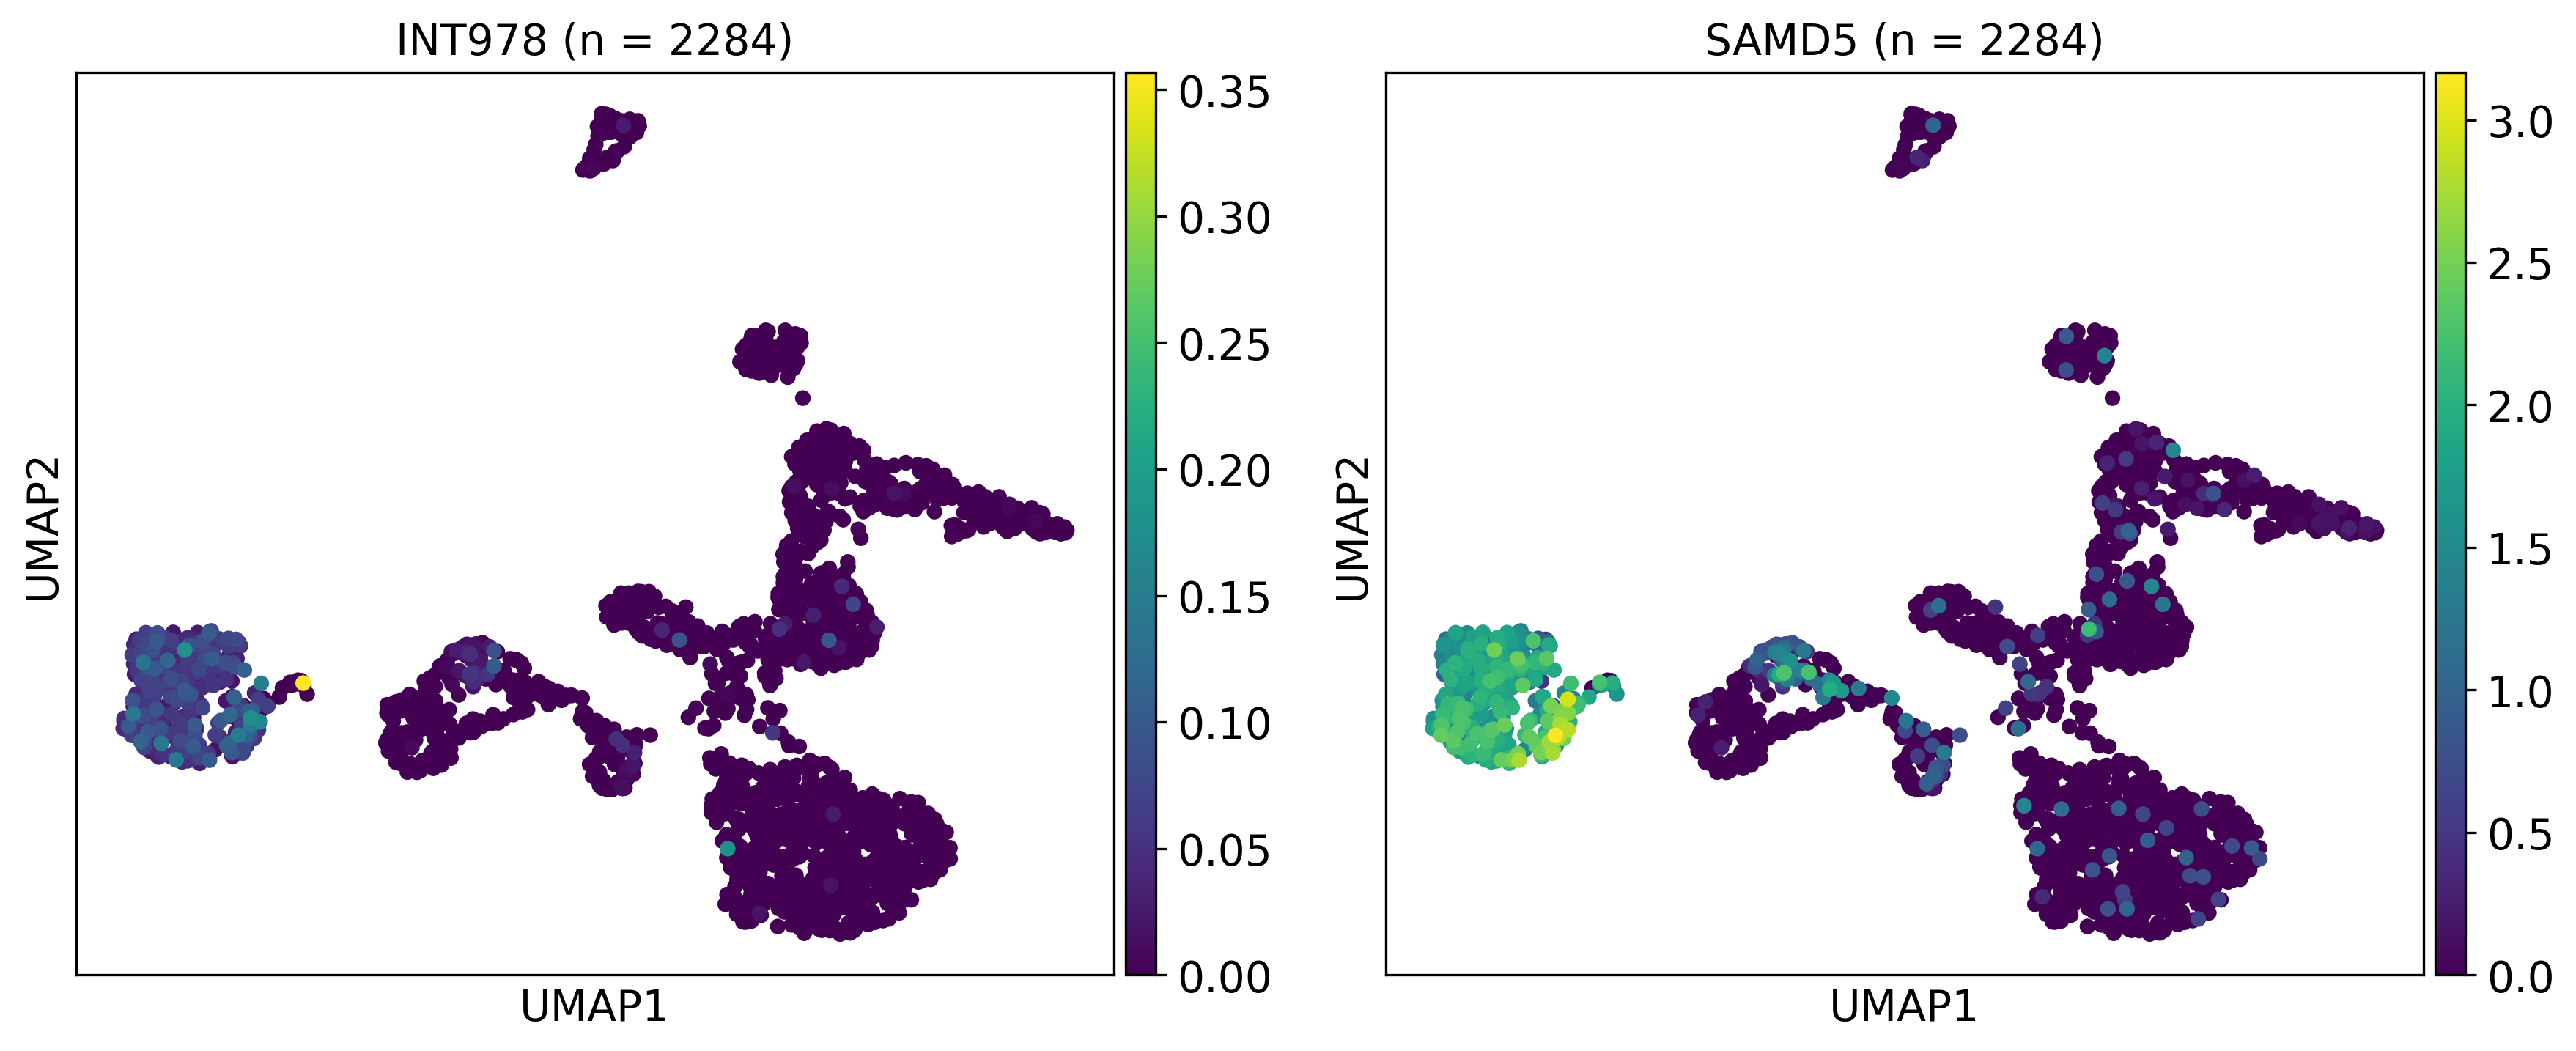
\includegraphics[width=\textwidth]{images/correlationUmaps/eye_3_SAMD5.png}
        \caption{Umaps of INT978 and SAMD5 (Spearman correlation 0.85) of the eye\_3 sample,
        intergenic region is on the opposite strand of the gene.}
    \end{subfigure}
    \caption{Correlation can be seen visually in UMAPs (colored by the normalized expression of the genes), here couple of examples given.}
    \label{fig:correlationUmaps}
\end{figure}



\subsection{Isolated intergenic regions}

The intergenic regions that are distant from known genes and contain reads may indicate novel genes.
To determine whether these are genuine signals rather than artifacts, several aspects were considered:
\begin{enumerate}
  \item Differential expression: Are these regions differentially expressed in any samples, i.e., are they specific to certain cell types?
  If so, this strongly suggests a biological origin rather than an artifact.
  %\item AT-rich sequences: Do nearby sequences contain 10 consecutive A/Ts?
  %Since primers bind to poly-A tails, such sequences found nearby could suggest
  %that observed peak of reads result from mispriming in longer unannotated gene.
  \item Open chromatin: Are open chromatin regions present upstream? Such regions often indicate active transcription.
  \item Conservation score: Coding regions tend to be more evolutionarily conserved than non-coding regions.
  \item Gene predictions: Do these regions overlap with predicted genes identified by computational tools?
\end{enumerate}

mention something about correlation and poly A segments.

\paragraph{Differential expression analysis}

To assess differential expression, all data samples were first clustered.
For \textit{PBMC\_10x} samples, clustering and cell annotation were performed using CellTypist.
For other samples, the Leiden algorithm was used, with manually chosen parameters to ensure a comparable number of clusters across similar datasets.
For instance, all \textit{lung} samples were clustered into five groups, aligning approximately with visible UMAP structures.
The UMAP visualizations, colored by clusters, can be found in Appendix \ref{fig:clusterings}.

After filtering those regions that were differentially expressed (tresholds were used 0.01 for adjusted p-value and 0.5 for 'logfoldchange'),
the 29 differentially expressed isolated intergenic regions were found.
Some examples can be seen in Figure \ref{fig:isolatedDGE}.

\begin{figure}[htbp]
\centering
\begin{tabular}{cc}
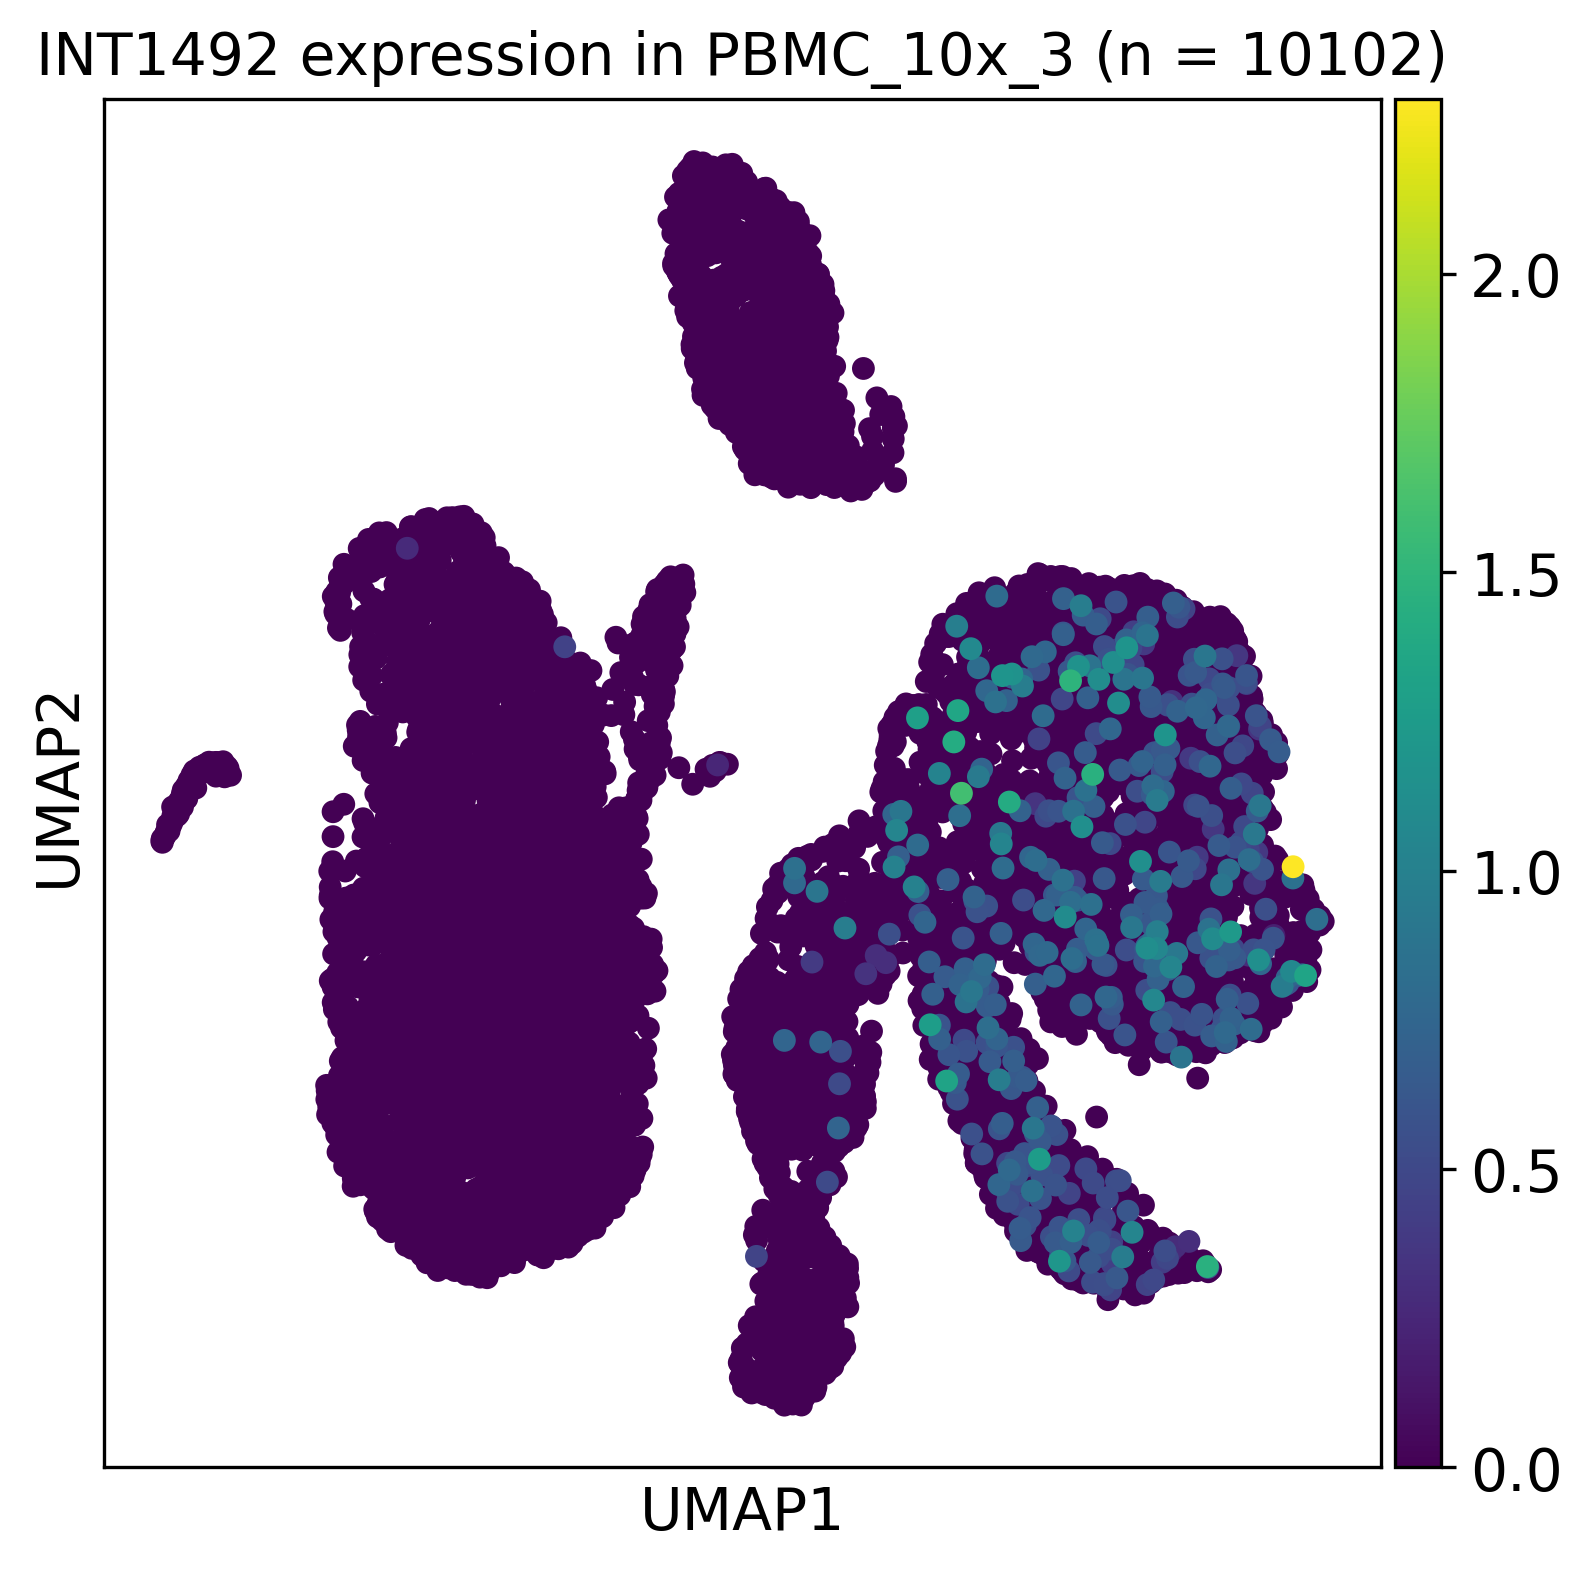
\includegraphics[width=0.45\textwidth]{images/isolatedDGEexamples/INT1492_PBMC_10x_3.png} &
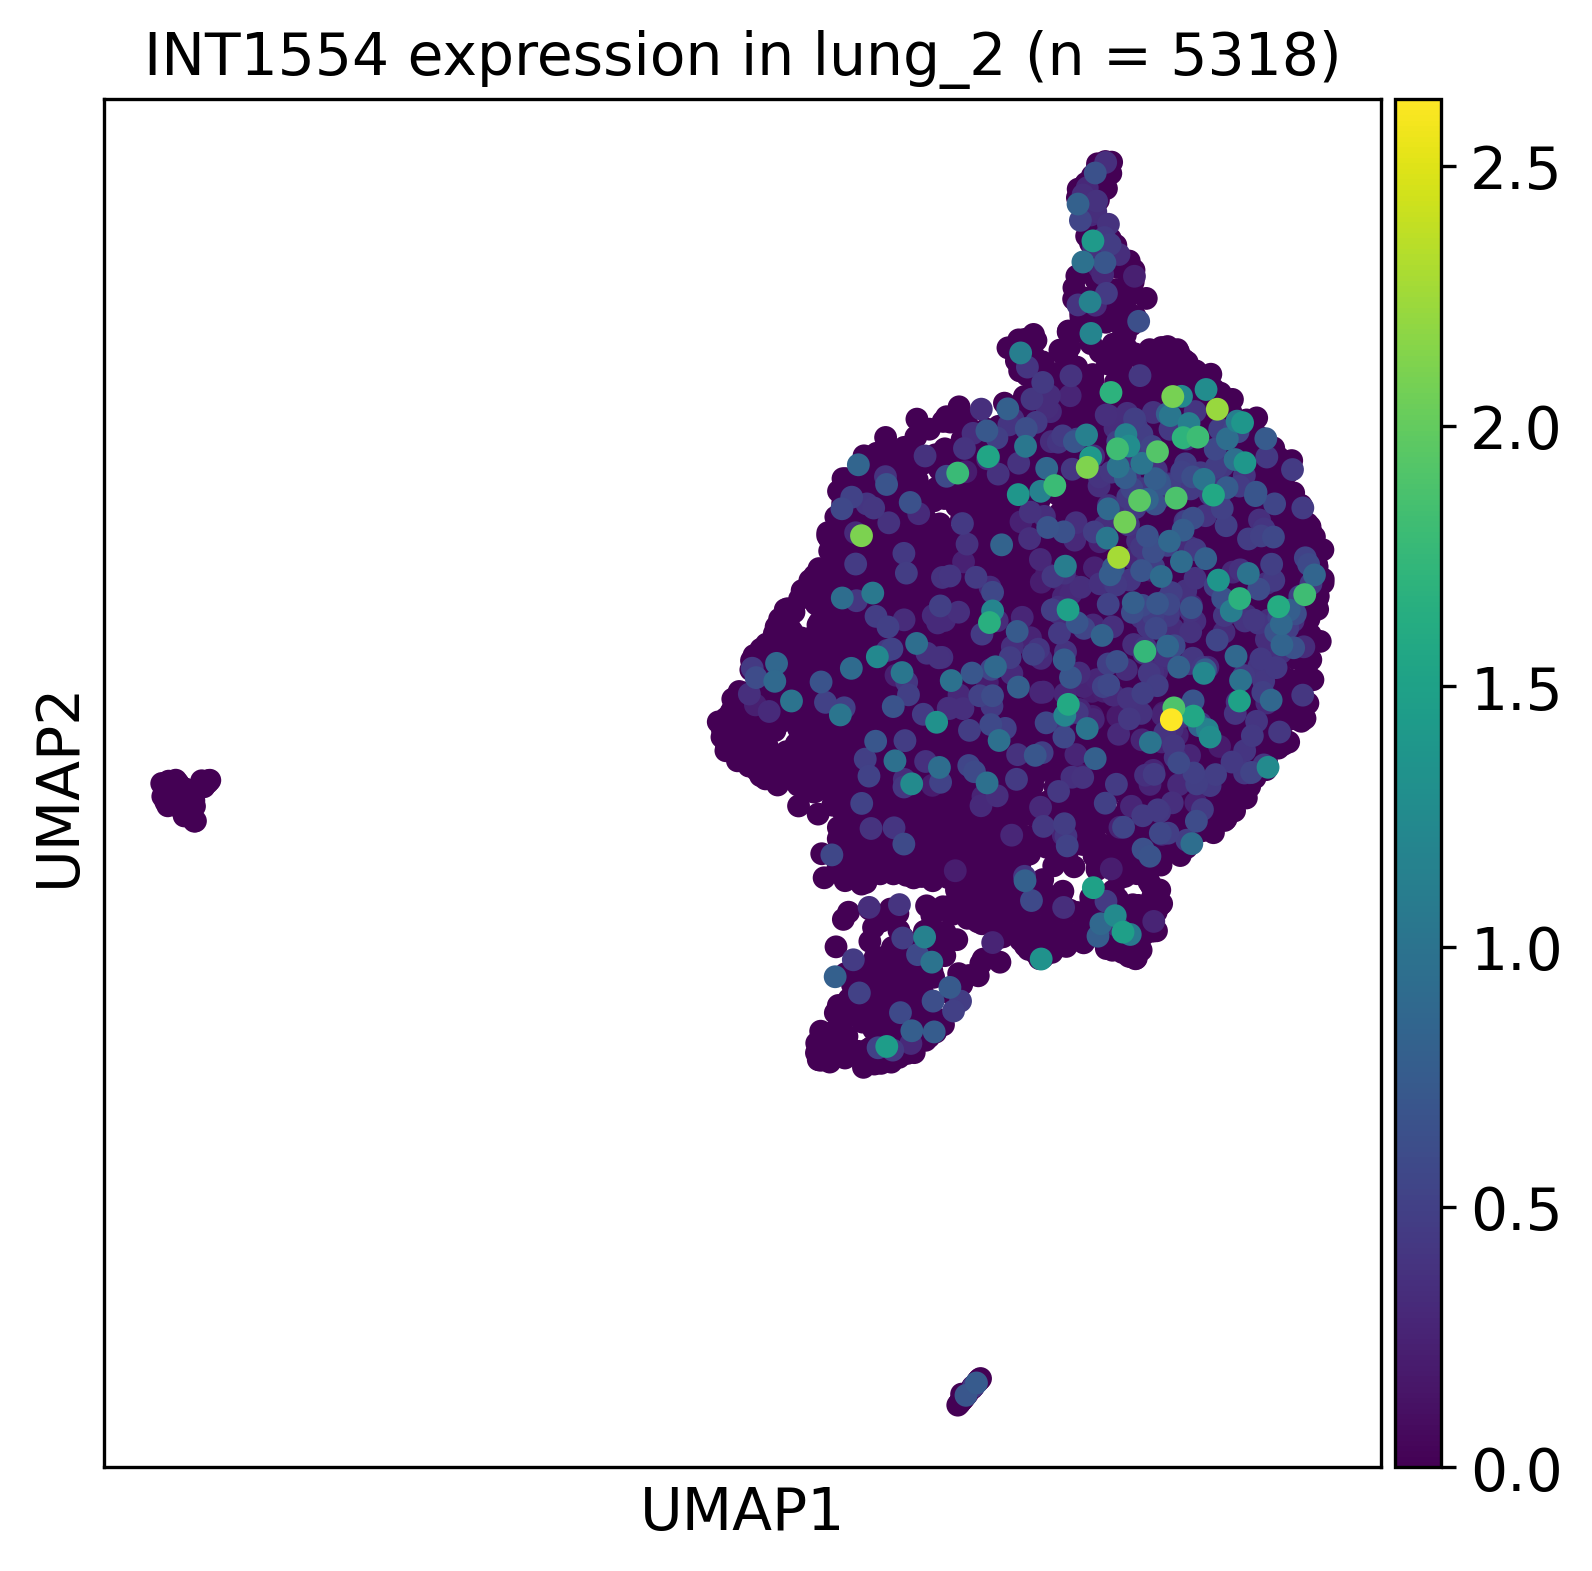
\includegraphics[width=0.45\textwidth]{images/isolatedDGEexamples/INT1554_lung_2.png} \\
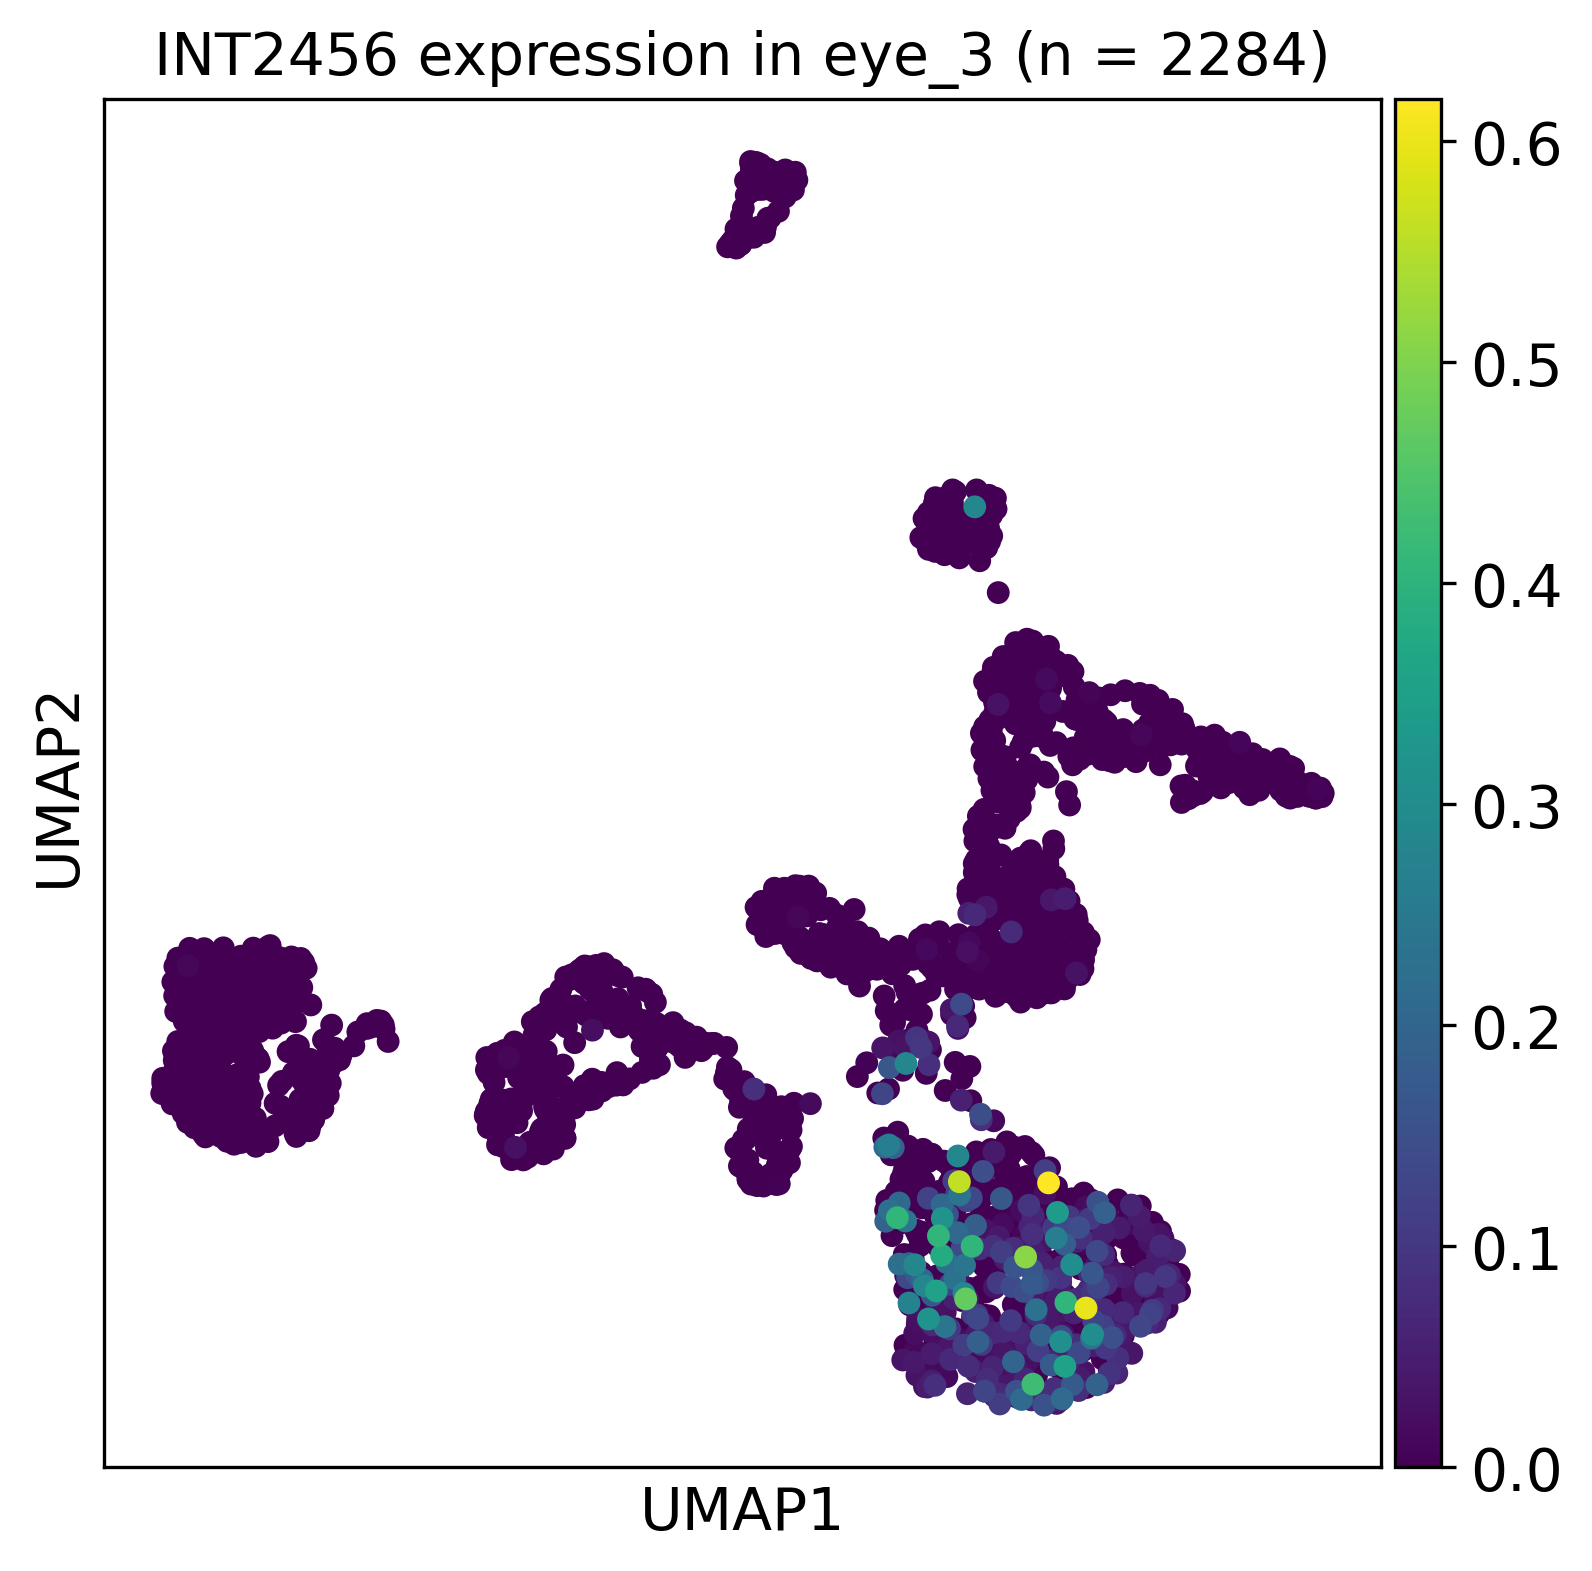
\includegraphics[width=0.45\textwidth]{images/isolatedDGEexamples/INT2456_eye_3.png} &
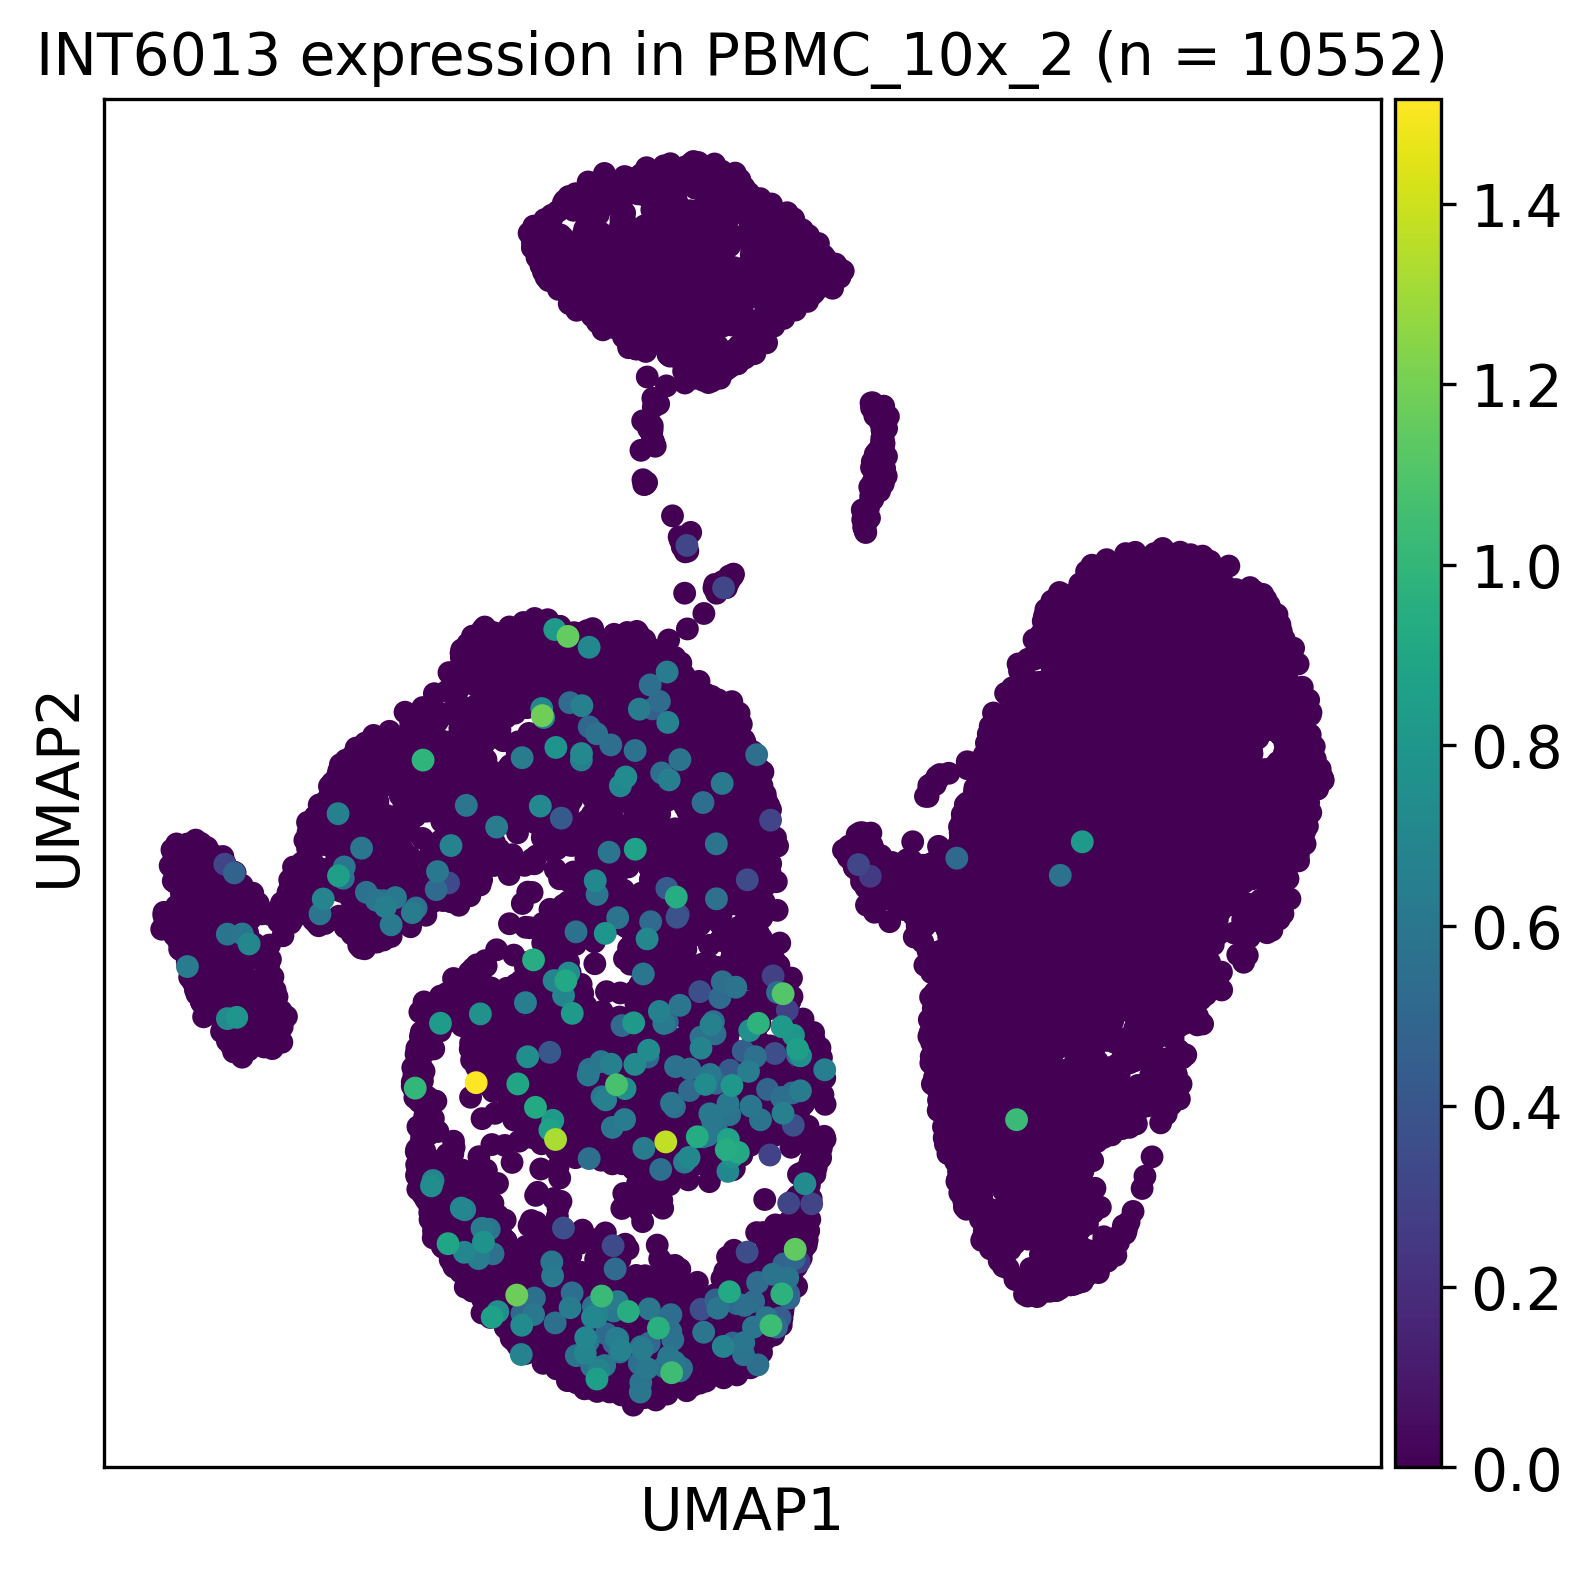
\includegraphics[width=0.45\textwidth]{images/isolatedDGEexamples/INT6013_PBMC_10x_2.png} \\
\end{tabular}
\caption{Examples of differentially expressed isolated intergenic regions.}
\label{fig:isolatedDGE}
\end{figure}

\iffalse
\paragraph{AT-rich regions}

AT-rich regions (here defined as 10 consecutive A/Ts, allowing one mismatch) were identified upstream of the 3' ends of isolated intergenic regions,
with the first occurrence recorded.

The distances from isolated intergenic regions to the nearest AT-rich sequences varied, with a mean of 938.537 and a median of 508.
The distribution is shown in Figure \ref{fig:distancesATrich}.
To determine whether these distances support the hypothesis that these locations are not random noise,
comparisons were made against 10,000 random genomic locations and 10,000 randomly selected gene 3' ends.
The results, summarized in Table \ref{tab:distancesATrich},
indicate that distances are larger for both randomly selected genes and random genomic locations.
Notably, distances from random locations to AT-rich sequences are shorter on average than those from randomly selected gene 3' ends.
This may be due to the fact that gene bodies, which typically lack AT-rich sequences, contribute to these distances.
Additionally, these results suggest that if small genes are indeed present between these isolated intergenic regions,
they should be relatively short.

\begin{table}[htbp]
  \centering
  \begin{tabular}{l|cc}
    \toprule
     & mean & median  \\
    \midrule
    isolated intergenic 3' ends & 938.537 & 508 \\
    3' ends of random genes & 1391.019 & 849 \\
    random locations & 1123.194 & 682 \\
    \bottomrule
  \end{tabular}
  \caption{The distances to the closest AT-rich regions.}
  \label{tab:distancesATrich}
\end{table}

\begin{figure}
  \centering
  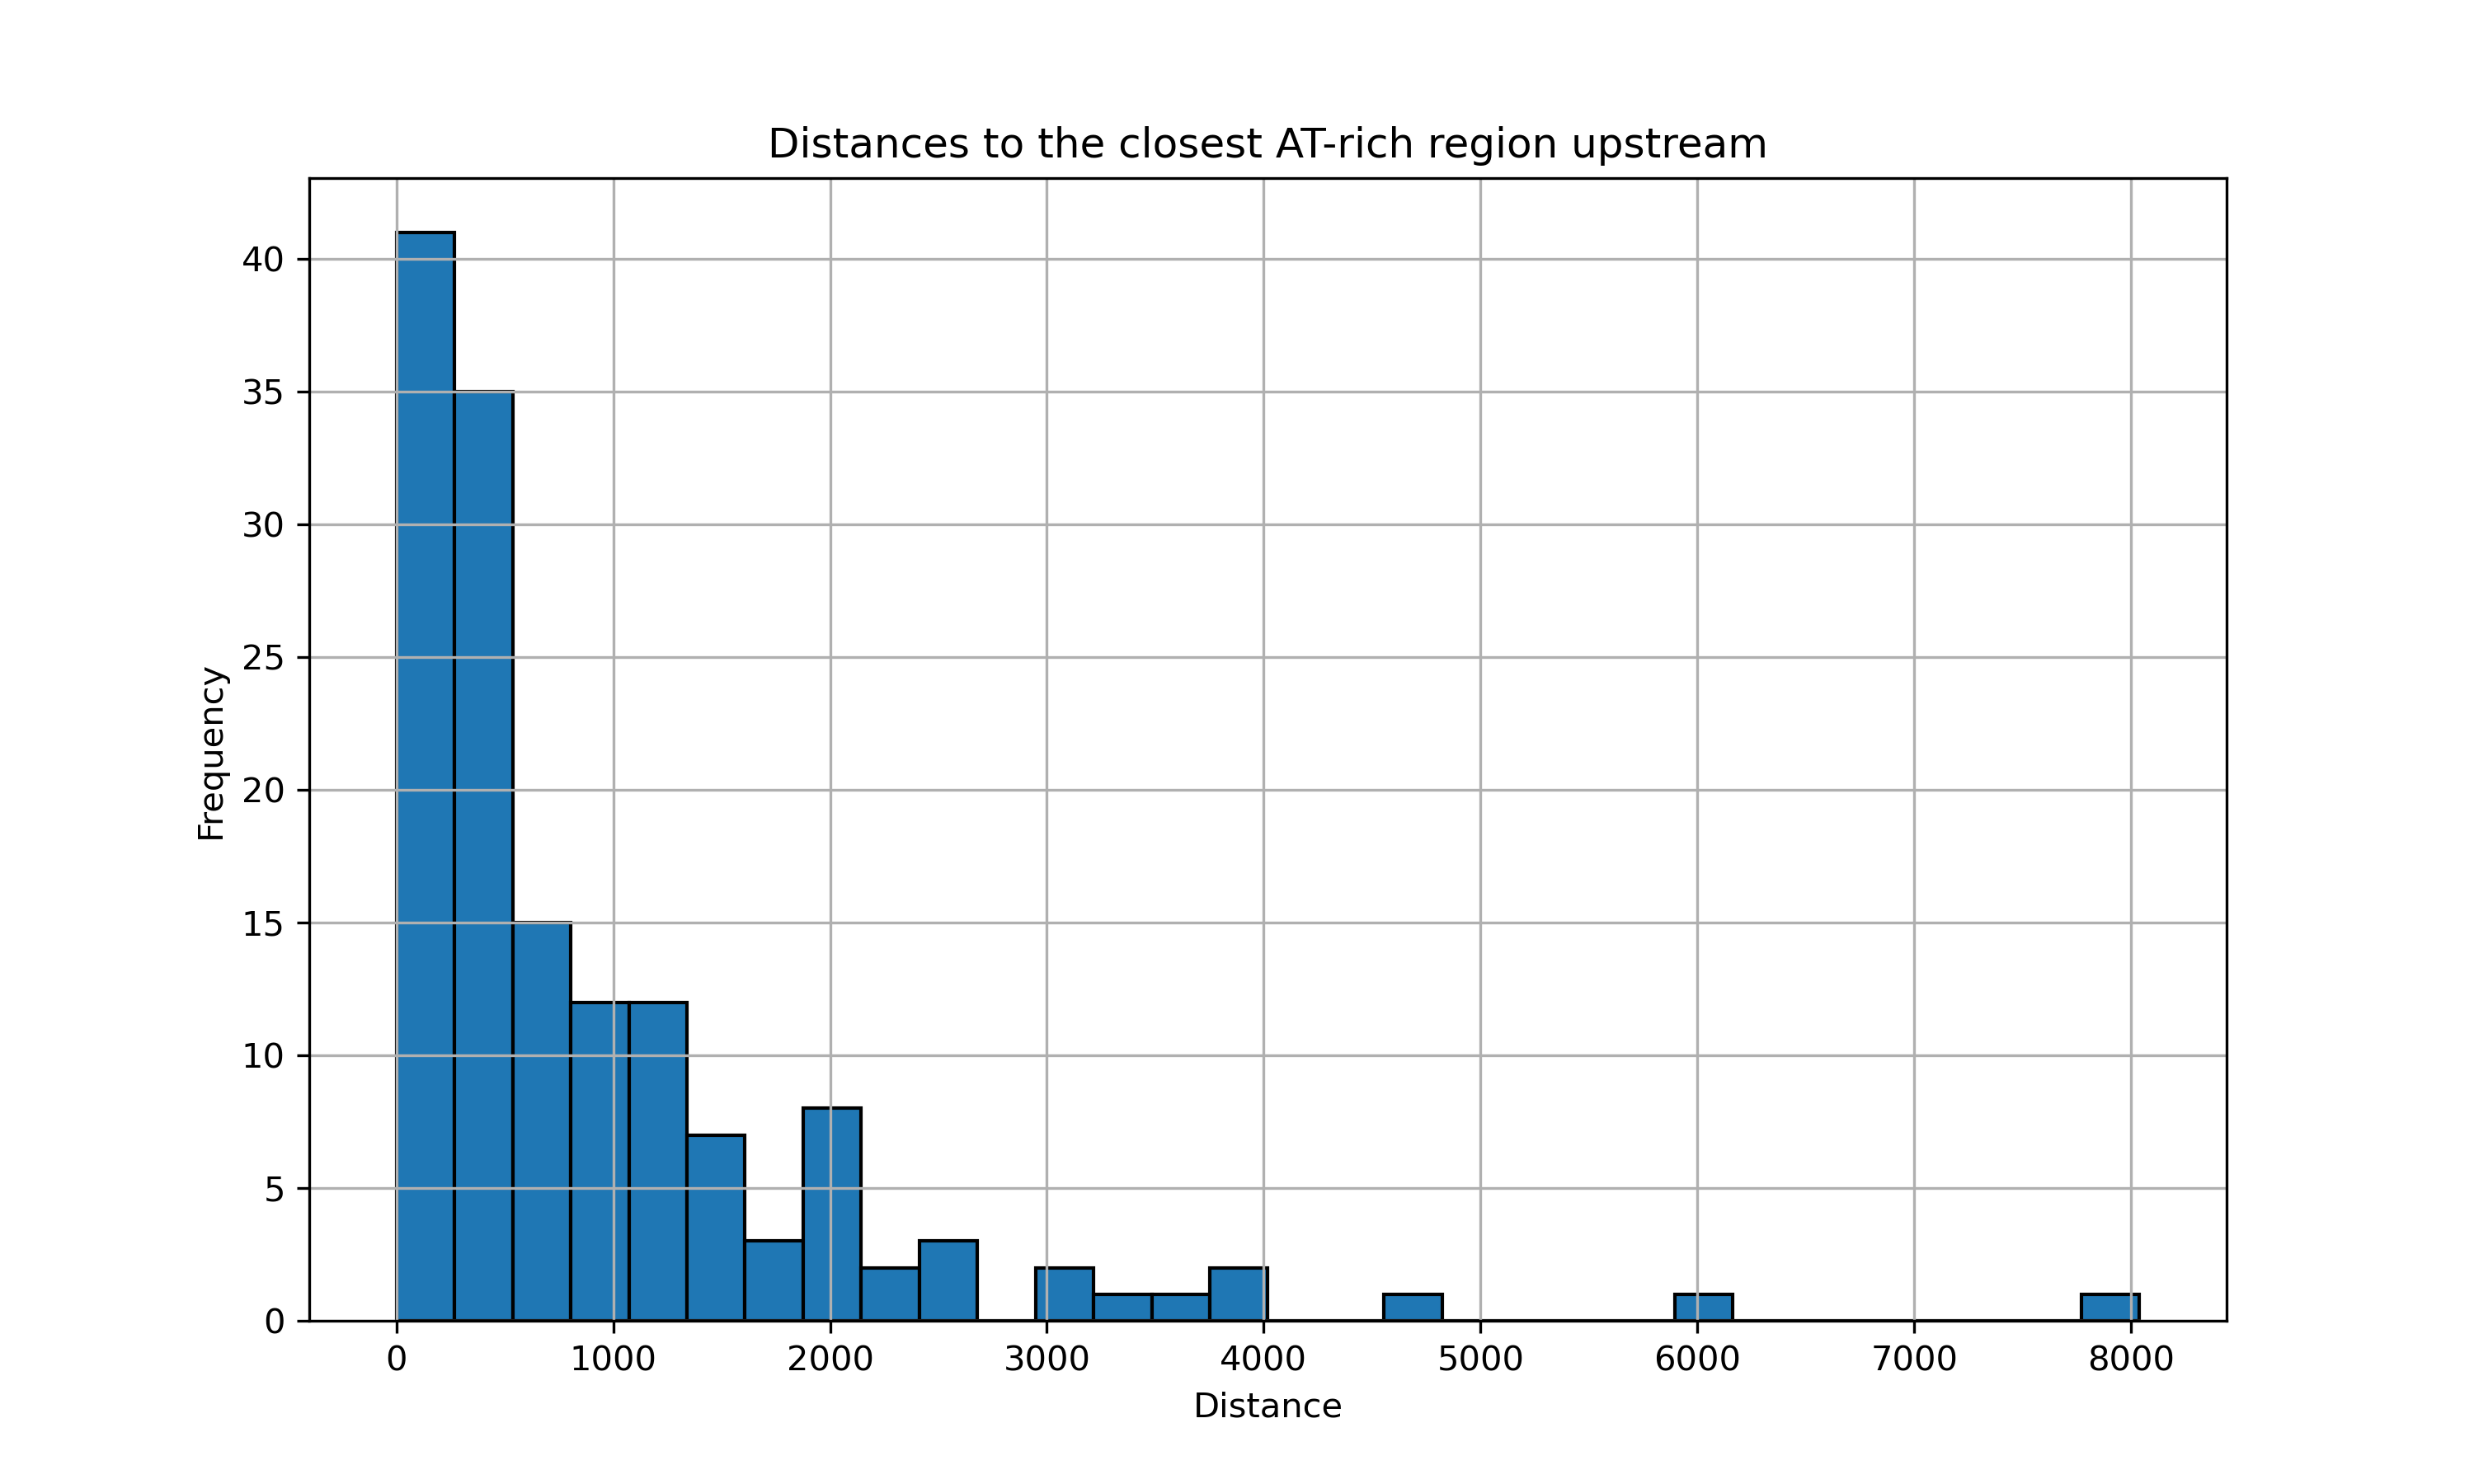
\includegraphics[width=\linewidth]{images/histogramATrich.png}
  \caption{Distances from 3' ends of isolated intergenic regions to closest AT-rich region upstream.}
  \label{fig:distancesATrich}
\end{figure}
\fi

\paragraph{Open chromatin}

Open chromatin regions may provide further evidence of transcriptional activity when located upstream.
However, distances to the nearest known genes must also be considered,
as upstream open chromatin sites may not be associated with the intergenic regions but rather with other genes.

For each intergenic region, distances to the nearest open chromatin sites and upstream genes (strand-unspecific) were calculated.
Of the 147 isolated intergenic regions, 66 had open chromatin regions closer than any known upstream genes.
To ensure that these sites were not merely associated with distant genes, an additional filter was applied, 
requiring that the closest open chromatin region be at least 2,000 bp from the nearest gene.
This yielded 40 intergenic regions.

\paragraph{Conservation scores}

A high conservation score in an intergenic region suggests potential functionality, providing additional evidence for biological relevance.
To identify such regions, those with conservation scores above 0.6 that did not overlap with known genes from references used were selected.
The resulting regions are presented in Table \ref{tab:conservedIntergenic}.

\begin{table}[h]
    \centering
    \begin{tabular}{lccc}
        \toprule
        Name & Genomic coordinates & Conservation score & Found in samples \\
        \midrule
        INT1216 & 1:72282700-72282900 & 0.7534172617 & brain, eye\\
	INT1829 & 1:77772950-77773050 & 0.6863111111 & lung \\
	INT2199 & 6:148122550-148122750 & 0.6364459652 & brain, eye \\
	INT2208 & 5:18162950-18163100 & 0.6138651685 & PBMC (indrops) \\
	INT3636 & X:129412750-129413050 & 0.7218984354 & brain \\
        \bottomrule
    \end{tabular}
    \caption{Conserved intergenic regions not overlapping with known genes from ncbi and gencode annotations.}
    \label{tab:conservedIntergenic}
\end{table}

\paragraph{Gene predictions}

To assess whether isolated intergenic regions overlap with predicted genes, UCSC gene prediction archives were examined,
focusing on overlaps with 3' ends of predicted genes.

Of the identified regions, 12 overlapped with predicted genes.
However, three of these did not overlap with the 3' ends of predicted genes,
which would be expected given that the data was generated using 3' end sequencing methods.
Five predicted genes were extensions of known genes,
while the remaining four corresponded to genes absent from RefSeq and NCBI references but supported by our data.
Table \ref{tab:predictedIsolated} summarizes these findings.
Only regions overlapping the 3' ends of predicted genes were considered as supported by gene prediction tools.

\begin{table}[h]
    \centering
    \begin{tabular}{llll}
        \toprule
        Name & Genomic coordinates & Prediction tool & Overlaps with 3' region of predicted gene \\
        \midrule
	INT196 & 6:89086200-89086500 & SIB & Yes (PNRC1) \\
	INT827 & 9:94111950-94112200 & SIB & Yes \\
	INT1216 & 1:72282700-72282900 & SIB & No (5' end) \\
	INT1387 & 11:63570800-63571050 & SIB & No \\
	INT1525 & 8:11842200-11842350 & SIB & Yes (CTSB) \\
	INT1801 & 5:151272550-151272700 & SIB & Yes (GM2A) \\
	INT2044 & 19:4041150-4041400 & SIB & Yes (ZBTB7A) \\
	INT4070 & 4:47430500-47430700 & SIB & Yes \\
	INT4147 & 1:34861500-34861700 & SIB & Yes (DLGAP3)\\
	INT4577 & 5:702050-702300 & SIB & Yes \\
	INT4948 & 5:703250-703450 & SIB & Yes \\
	INT5710 & 4:47428500-47428700 & SIB & No \\
        \bottomrule
    \end{tabular}
    \caption{Isolated intergenic regions overlapping with predicted genes from UCSC gene prediction archive.
    The gene in the brackets shows if the predicted gene is extended version of already annotated genes.}
    \label{tab:predictedIsolated}
\end{table}

\paragraph{Combining supporting features}

In total, five features were examined as supportive evidence for the biological significance of these intergenic regions:
conservation, AT-rich/open chromatin presence, differential expression, and gene predictions.
Based on these, four sublists of isolated intergenic regions were generated:

\begin{itemize}
  \item Conserved regions
  \item Regions associated with open chromatin
  \item Differentially expressed regions
  \item Regions overlapping predicted genes
\end{itemize}

Notably, the list of conserved regions did not intersect with the other three.
The predicted gene list had two regions in common with the differential expression list (INT196, INT1525)
and one in common with the open chromatin list (INT4147).
All three of these predicted genes were extended versions of already annotated genes (see example in Figure \ref{fig:predictedExtension}).
The differential expression and open chromatin lists had 11 regions in common
(INT1312, INT1426, INT1492, INT1554, INT1609, INT1993, INT2209, INT349, INT368, INT4216, INT6013).
No regions appeared in more than two lists.

\begin{figure}
  \centering
  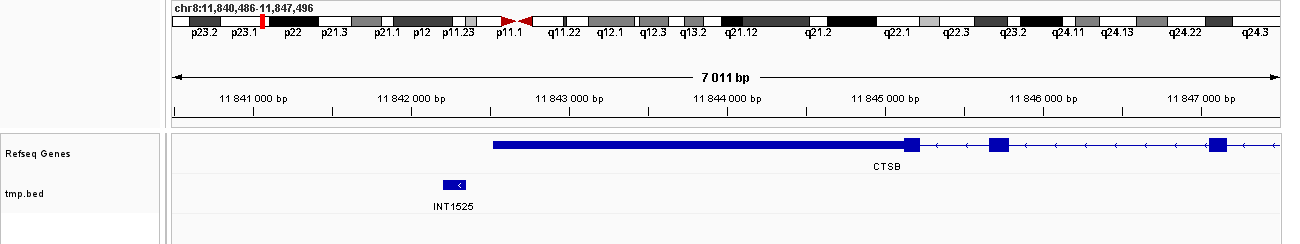
\includegraphics[width=\linewidth]{images/igv/INT1525.png}
  \caption{Example of gene which is predicted to have some longer transcripts than are present in the gencode and ncbi annotations.
  The intergenic region is located after the 3' end of gene CTSB, however,
  SIB prediction tool suggest that longer transcripts should be included in the annotation of this gene.}
  \label{fig:predictedExtension}
\end{figure}

\subsection{Antisense intergenic regions}

Interpretation of antisense intergenic regions is more complicated.
The features such as open chromatin, AT-richness or conservativness are not strand specific,
meaning that if they would be present, they could not be attributed with certainty for our intergenic regions.
The differential expression can be checked, however, even if the antisense intergenic region is differentially expressed,
it still can be an artifact, originating from differentially expressed transcripts.
Hence from the features checked for the isolated intergenic regions, only real supporting evidence would be computational gene prediction.

\paragraph{Gene predictions}

As in the case of isolated intergenic regions,
antisense intergenic regions were checked for overlaps with predicted genes from UCSC prediction archive.
There were 49 such regions found, out of them 35 were in the 3' ends of predicted genes.
9 of those 35 predicted genes were longer version of already annotated genes in RefSeq or GENCODE references.
The all list can be seen in the Table \ref{tab:predictionsAntisense}.

\begin{table}[h]
    \small
    \centering
    \begin{tabular}{llll}
        \toprule
        Name & Genomic coordinates & Prediction tool & Overlaps with 3' region of predicted gene \\
        \midrule
	INT7 & 6:24718850-24719100 & SIB & Yes \\
	INT33 & 5:172767250-172767500 & SIB & Yes (DUSP1) \\
	INT134 & 15:41280550-41280800 & SIB & Yes (extends a bit after) \\
	INT218 & 5:61409150-61409400 & SPG & No (5' end) \\
	INT285 & 10:110898200-110898550 & SIB & Yes (BBIP1) \\
	INT327 & 1:169132100-169132350 & SIB & Yes (NME7) \\
	INT347 & 14:75277700-75278000 & Gescan & No \\
	INT382 & 12:11892250-11892500 & Gescan & Yes \\
	INT386 & 6:26215200-26215450 & SIB & Yes (H2BCB?) \\
	INT438 & 4:39713300-39713600 & SIB & Yes (almost all (short) gene spanned) \\
	INT533 & 8:130110900-130111150 & SIB & Yes \\
	INT617 & 15:85733950-85734200 & SIB & Yes \\
	INT621 & 9:75148850-75149400 & SIB & Yes (OSTF1) \\
	INT651 & 1:28579100-28579350 & SIB & Yes (TRNAU1AP) \\
	INT654 & 6:34382850-34383050 & SIB & No (but short gene)\\
	INT828 & 8:133035800-133036050 & SIB & Yes (SLA) \\
	INT859 & 2:71373500-71373750 & SIB & No (slight overlap on 5' end) \\
	INT898 & 17:51190400-51190700 & SIB & Yes (extends after)\\
	INT903 & 8:22613400-22613650 & SIB & Yes \\
	INT949 & 9:111693050-111693400 & SIB & Yes \\
	INT972 & 15:64954800-64955350 & SIB & Yes \\
	INT984 & 18:63291900-63292200 & Geneid & Yes \\
	INT1028 & 5:50414200-50414500 & SIB & Yes \\
	INT1155 & 1:36296050-36296300 & SIB & No (5' end) \\
	INT1231 & 10:19890700-19891050 & Gescan & Yes \\
	INT1402 & 5:142786700-142786950 & SIB & No (5' end) \\
	INT1440 & 2:235746450-235746700 & SIB & Yes \\
	INT1445 & 9:40885650-40885900 & SIB & Yes \\
	INT1548 & 7:50342700-50342950 & Gescan & No (exon in the middle) \\
	INT1616 & 17:30895450-30895700 & SIB & No (5' end) \\
	INT1749 & 3:172333550-172333750 & SIB & No (5' end) \\
	INT1931 & 17:82522100-82522350 & SIB & Yes \\
	INT2065 & 10:103606150-103606400 & SIB & Yes \\
	INT2158 & 14:49636100-49636350 & SIB & No (5' end, DNAAF2) \\
	INT2194 & 7:130521250-130521500 & SIB & No (but gene is short) \\
	INT2371 & 1:14632650-14632900 & Geneid & No (middle exon) \\
	INT2380 & 22:33853900-33854150 & Geneid & Yes \\
	INT2825 & 13:45300050-45300300 & Geneid & No (middle exon) \\
	INT2979 & 4:98929350-98929600 & SIB & No (5' end, EIF4E) \\
	INT3328 & 2:184604250-184604500 & SIB & Yes \\
	INT3429 & 17:48172750-48173150 & Augustus & Yes \\
	INT3504 & 15:25332950-25333150 & SIB & Yes (UBE3A) \\
	INT3849 & 3:121432200-121432400 & SIB & Yes \\
	INT3868 & 17:31448500-31448700 & SIB & Yes \\
	INT4458 & 5:44820700-44820900 & SIB & Yes (MRP530) \\
	INT4743 & 20:3188900-3189050 & SIB & Yes (DDRGK1) \\
	INT5002 & 11:92232750-92232950 & SIB & Yes \\
	INT5315 & 20:3183750-3184050 & SIB & Yes \\
	INT5329 & 13:95603000-95603200 & SIB & Yes (extends after) \\
        \bottomrule
    \end{tabular}
    \caption{Antisense intergenic regions overlapping with predicted genes from UCSC gene prediction archive.
    The gene in the brackets shows if the predicted gene is extended version of already annotated genes.}
    \label{tab:predictionsAntisense}
\end{table}

\paragraph{Poly-A segments}

Having in mind that majority of the antisense intergenic regions have poly-A stretch after 3' end,
and some of them strongly correlates with genes on the opposite strands,
it is possible that they are artefacts from the library preparation.
Particularly, it could happen that poly-T primer binds to poly-A stretch of cDNA produced by other primer,
and in such way inversed trnascripts are produced,
which are later mapped to antisense strands of a known gene (see Figure \ref{RTtemplateswitch}).











\iffalse

Firstly, to check if the intergenic regions contain any biologically meaningfull information,
for each sample cells were clustered based only on those intergenic samples.
As can be seen in some provided examples in Figure \ref{fig:intergenicClustering},
clustering can be seen in this case and it roughly corresponds to the clustering using standard ('10x') annotation.
This shows that biologically meaningful information is indeed present in those intergenic regions,
Hence, further analysis were performed on those intergenic regions.

The intergenic regions from all samples were combined into one list, resulting in a list of 13667 entries.
For each region several metrics were calculated, including mean CPM (counts per million) per sample,
the number of samples in which this region was detected, conservation score.
Additionally it was checked if those regions overalap with any genes predicted by gene predictions tools,
also, closest genes on the same and opposite strands (and distances from them) were found.
The list was filtered based on the numer of samples the region was detected, allowing only those regions that are detected in all
blood, brain, eye, or lung samples (with the exception for PBMC samples,
for them more permissive filtering was applied, allowing those entries that were detected only by one sequencing protocol as well,
i.e. it could be detected in all 'PBMC\_10x samples' or all 'PBMC\_indrops samples').
This resulted in a filtered list of 2590 intergenic regions.

Since the filtered list still remained huge, additional filtering criterions were applied:
\begin{itemize}
  \item \textbf{Conservation scores.} Since the conservation scores are not strand specific,
  it makes no sense to filter out directly by the conservation score, because in the case there is other gene on the opposite strand
  of defined region, the high conservation score could be induced by this other gene.
  However, if there are no overlapping genes, high conservation score of an intergenic region could suggest that it might have some function.
  Therefore, a group of possibly biologically meaningful locations were extracted by filtering those genes that have high conservation score
  (threshold was set to 0.6) and do not overlap with any known genes (from the ncbi or genecode references).
  \item \textbf{Gene predictions tools.} There are tools that predict genes based on the genomic sequence.
  Such predictions (if overlapping with defined intergenic regions) would support the claim that
  those (overlapping) intergenic regions are not noise, especially if the intergenic peaks would overlap with 3' ends of predicted genes.
  \item \textbf{Intergenic region specificity.} In the case the reads from specific regions are present only in one cell group,
  the biological origin of these reads are very likelly.
  Such specific regions can be noticed using differential gene expression analysis,
  i.e. checking how gene (or in our case, intergenic region) expression varies between different cell types.
  \item \textbf{ATAC data.} ATAC data can show open chromatin regions, which are typically associated with active transcription.
  If the intergenic regions overlap with open chromatin regions, this could provide additional evidence that reads from this region is not noise.
  \item \textbf{Correlations with nearby genes.} If there exist correlations between the expression of the intergenic regions
  and expression of nearby genes, that could suggest that those regions are not noise and are involved in the same pathways as their neighbours.
\end{itemize}

In the following subsections I will explore genes filtered by those strategies separatelly.

\begin{figure}[htbp]
    \centering
    \begin{subfigure}{0.45\textwidth}
        \centering
        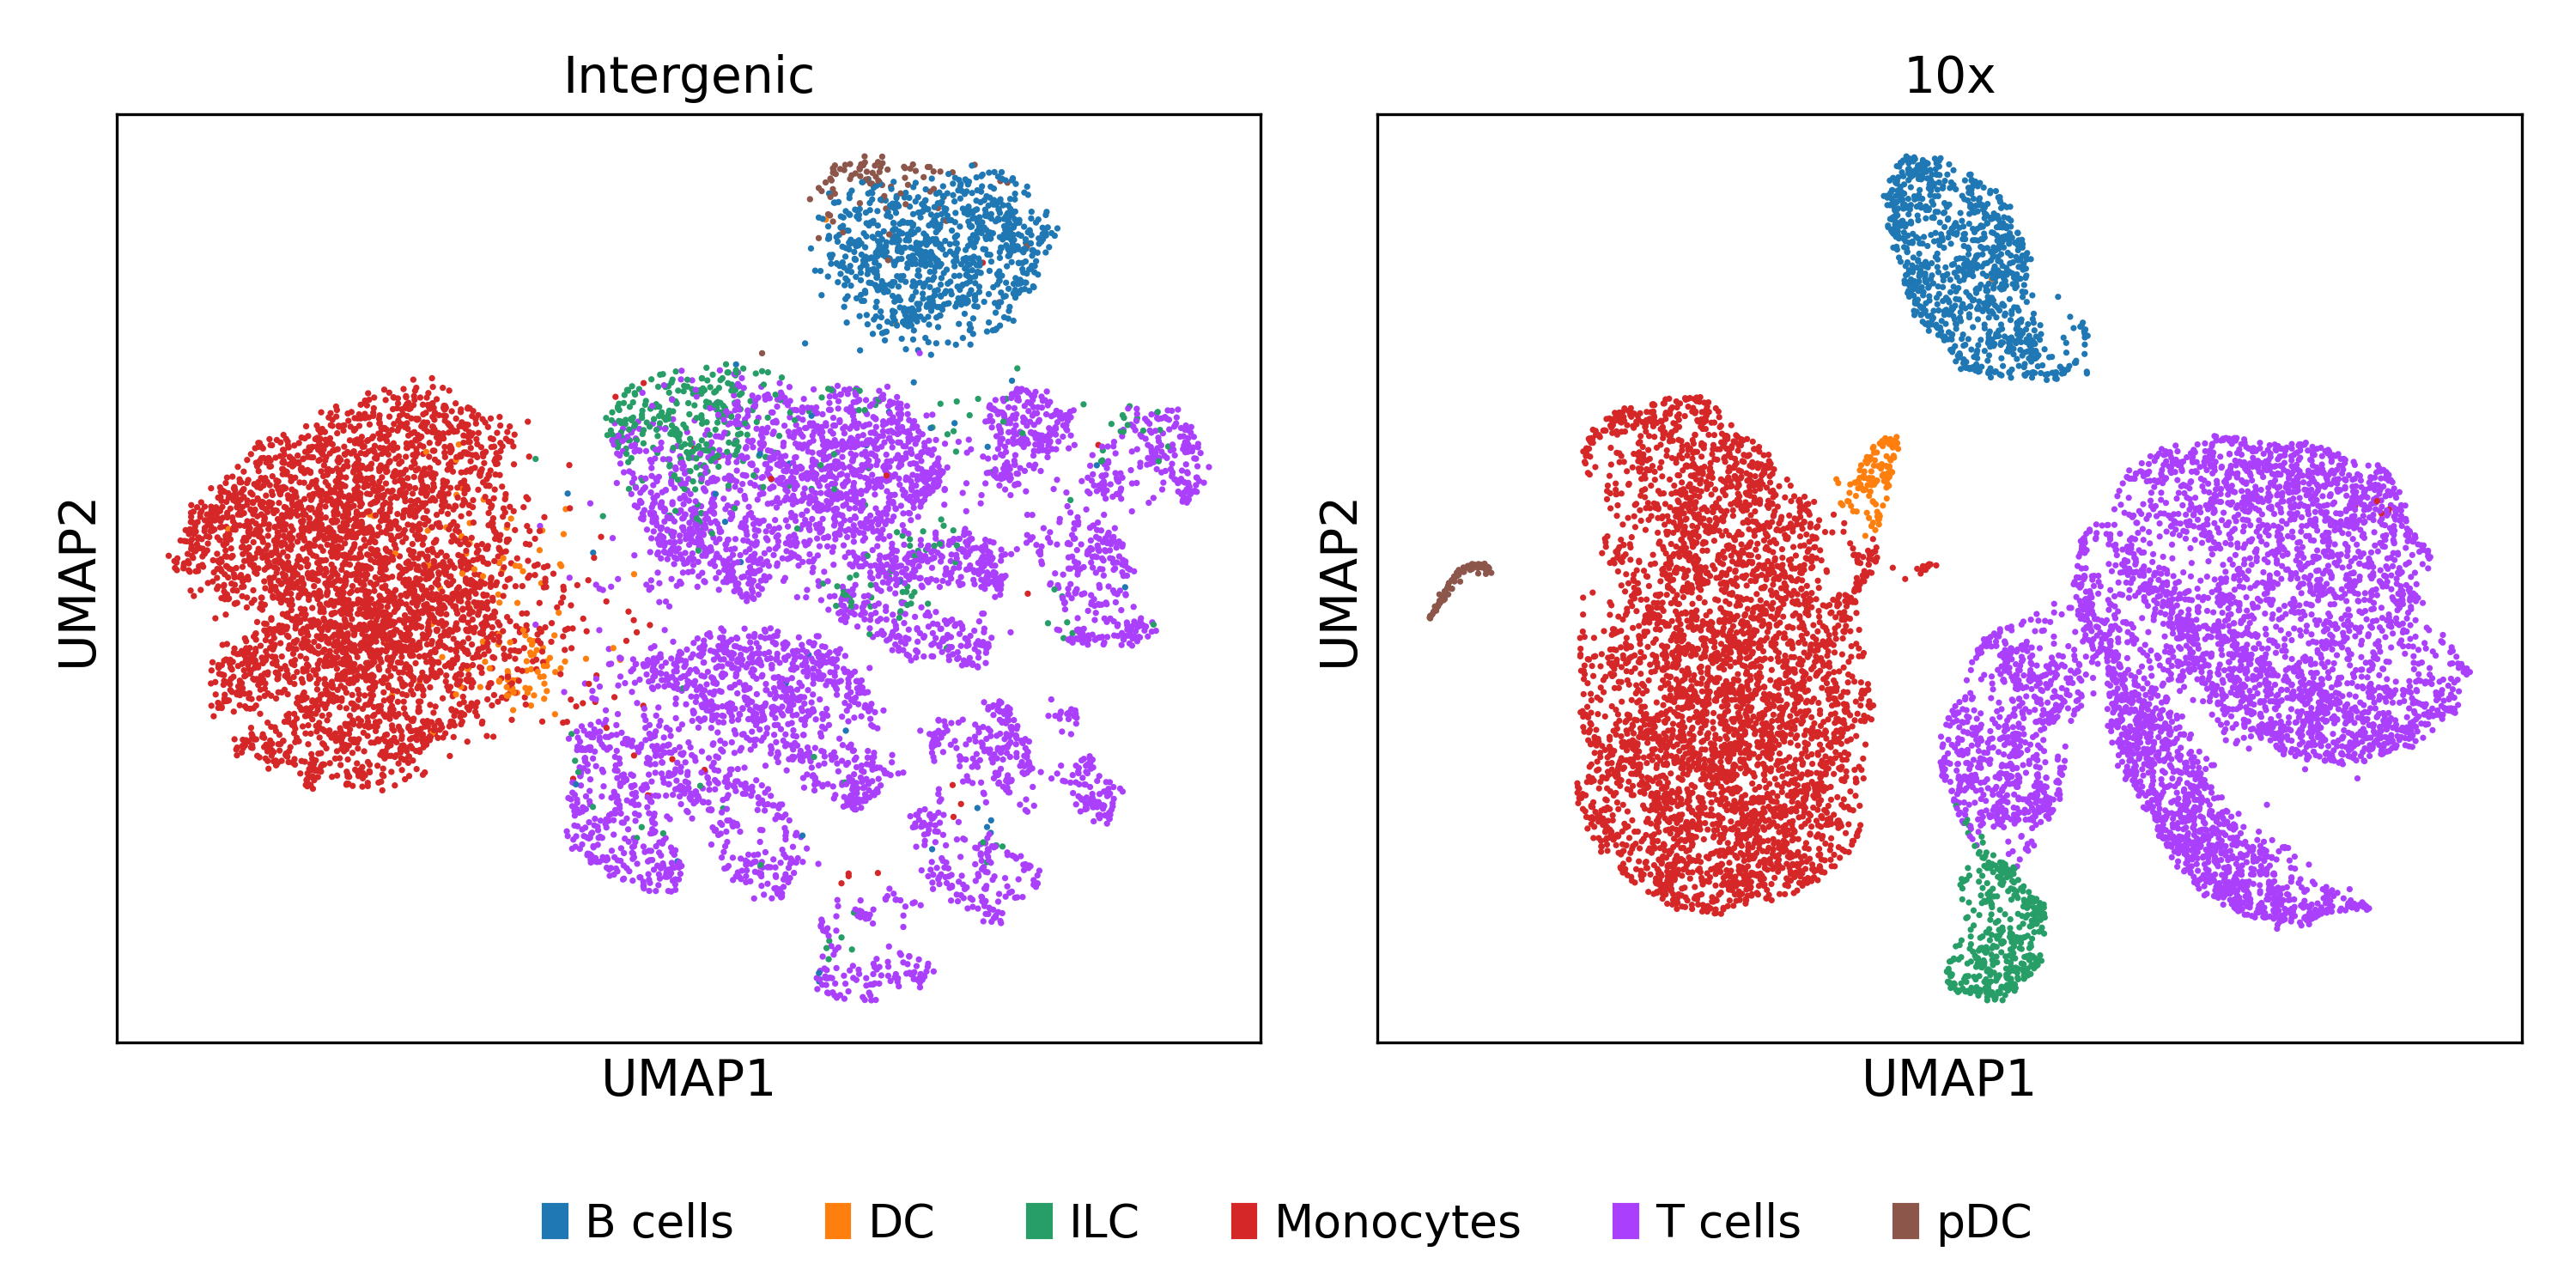
\includegraphics[width=\textwidth]{images/umaps/intergenic_10x_pbmc10x3.png}
        \caption{10x PBMC 3}
    \end{subfigure}
    \hfill
    \begin{subfigure}{0.45\textwidth}
        \centering
        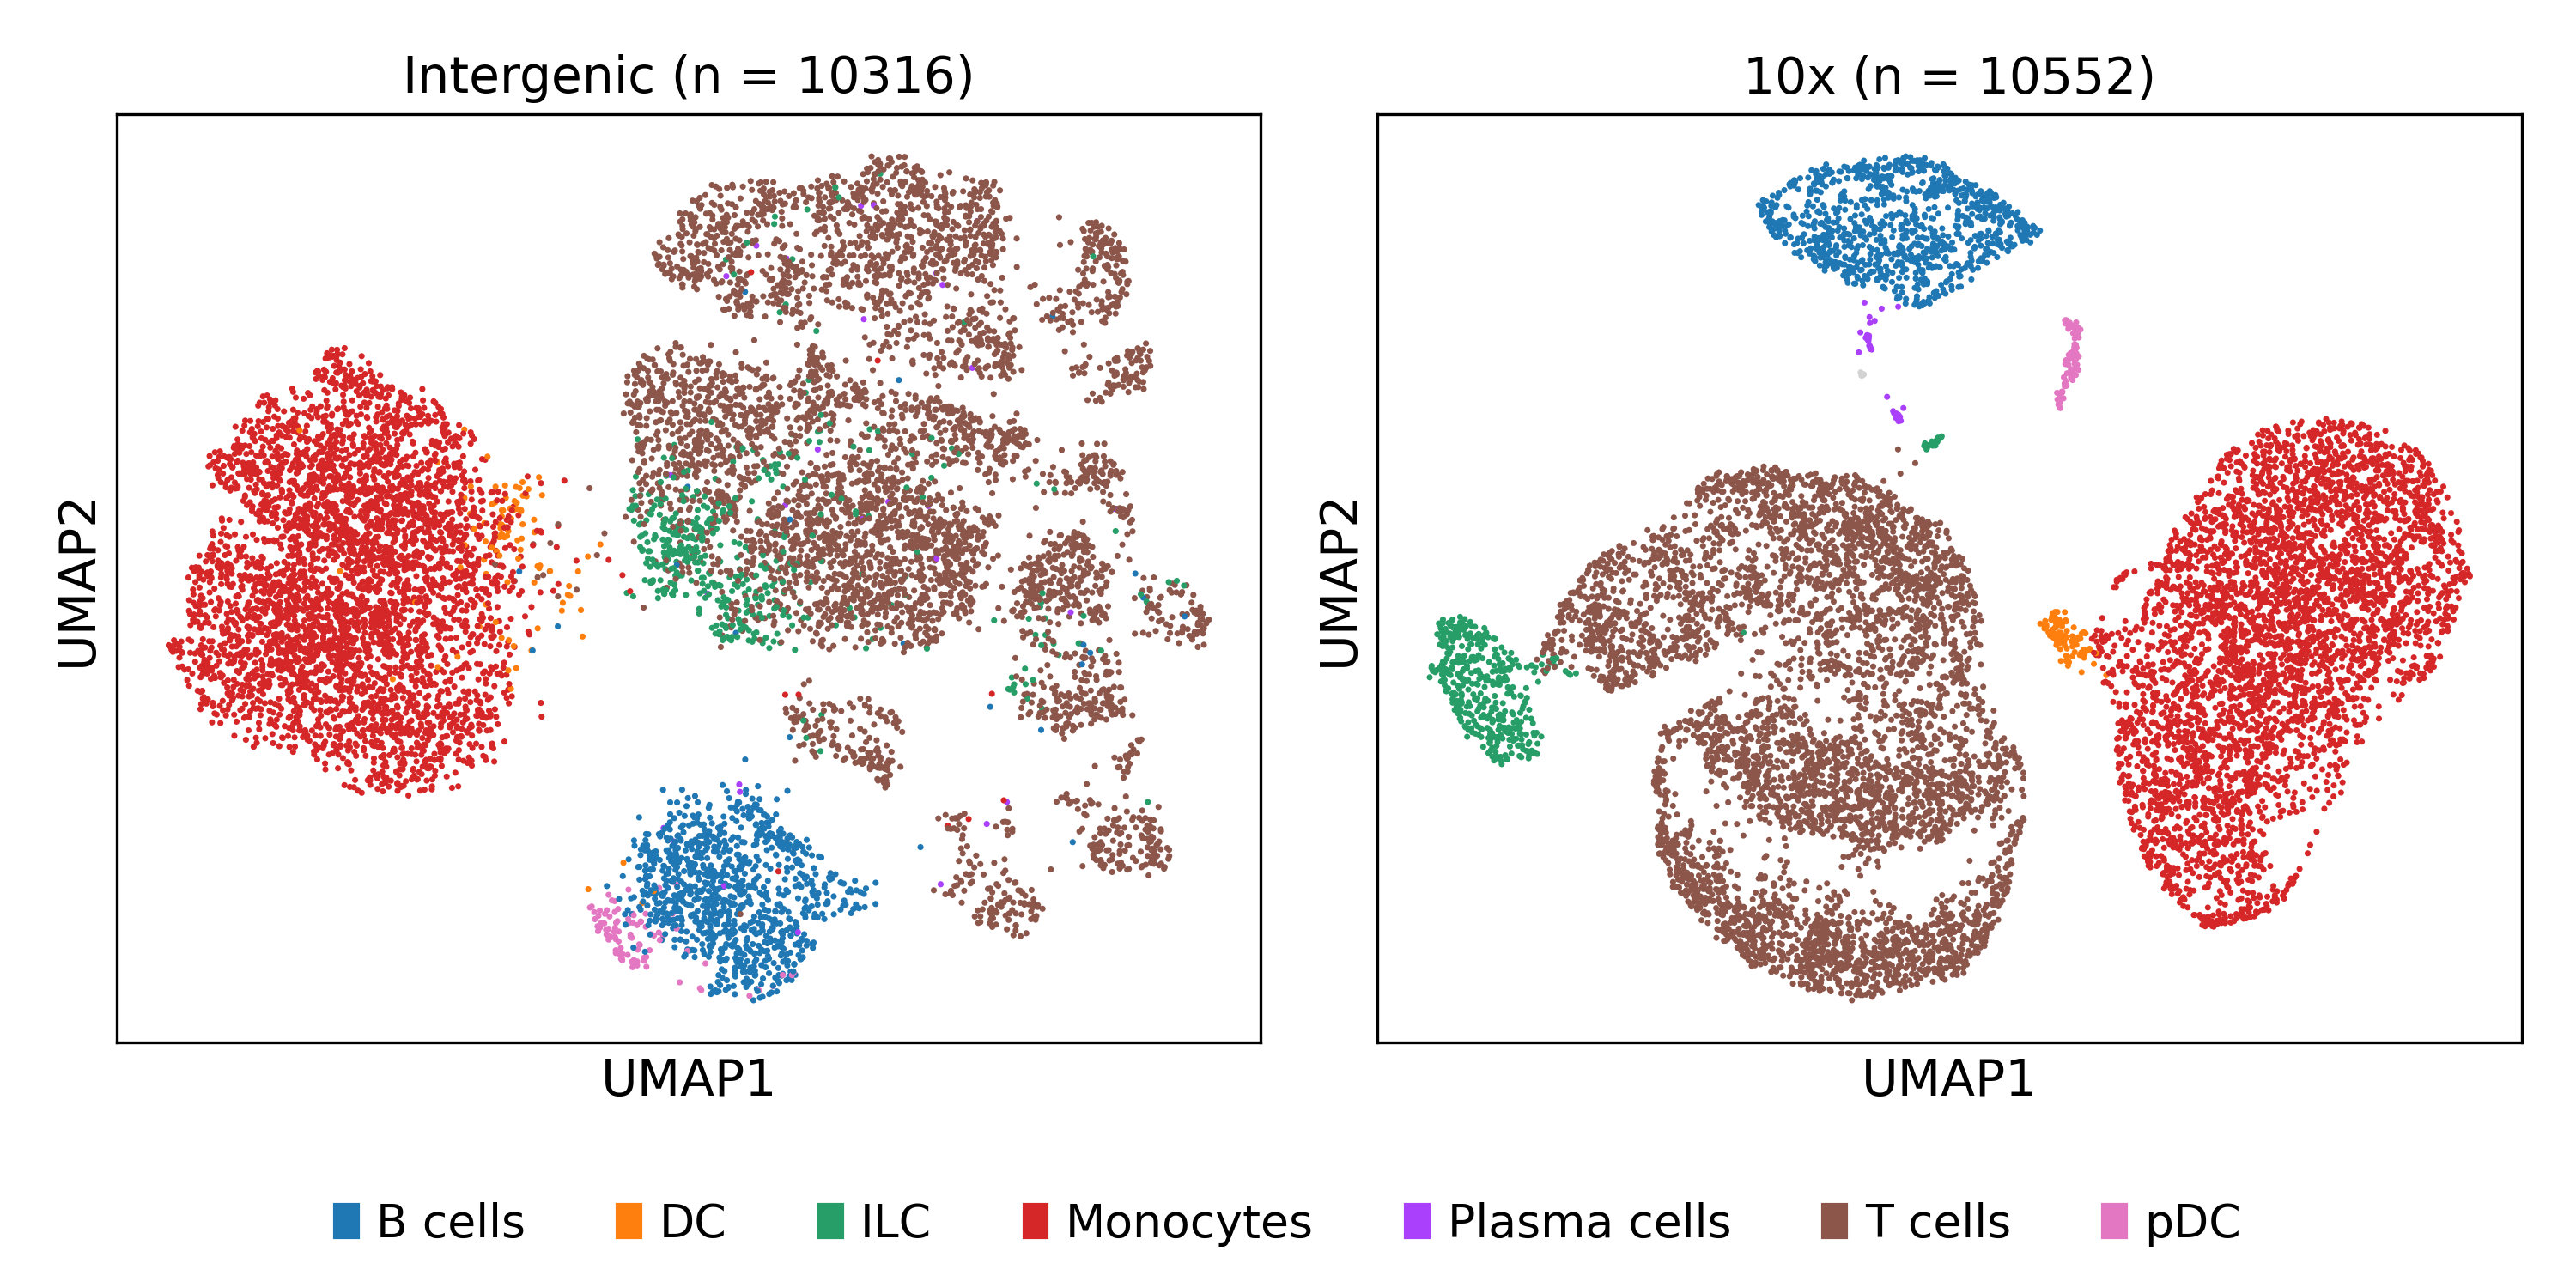
\includegraphics[width=\textwidth]{images/umaps/intergenic_10x_pbmc10x2.png}
        \caption{10x PBMC 2}
    \end{subfigure}
    \vspace{0.5em}
    \begin{subfigure}{0.45\textwidth}
        \centering
        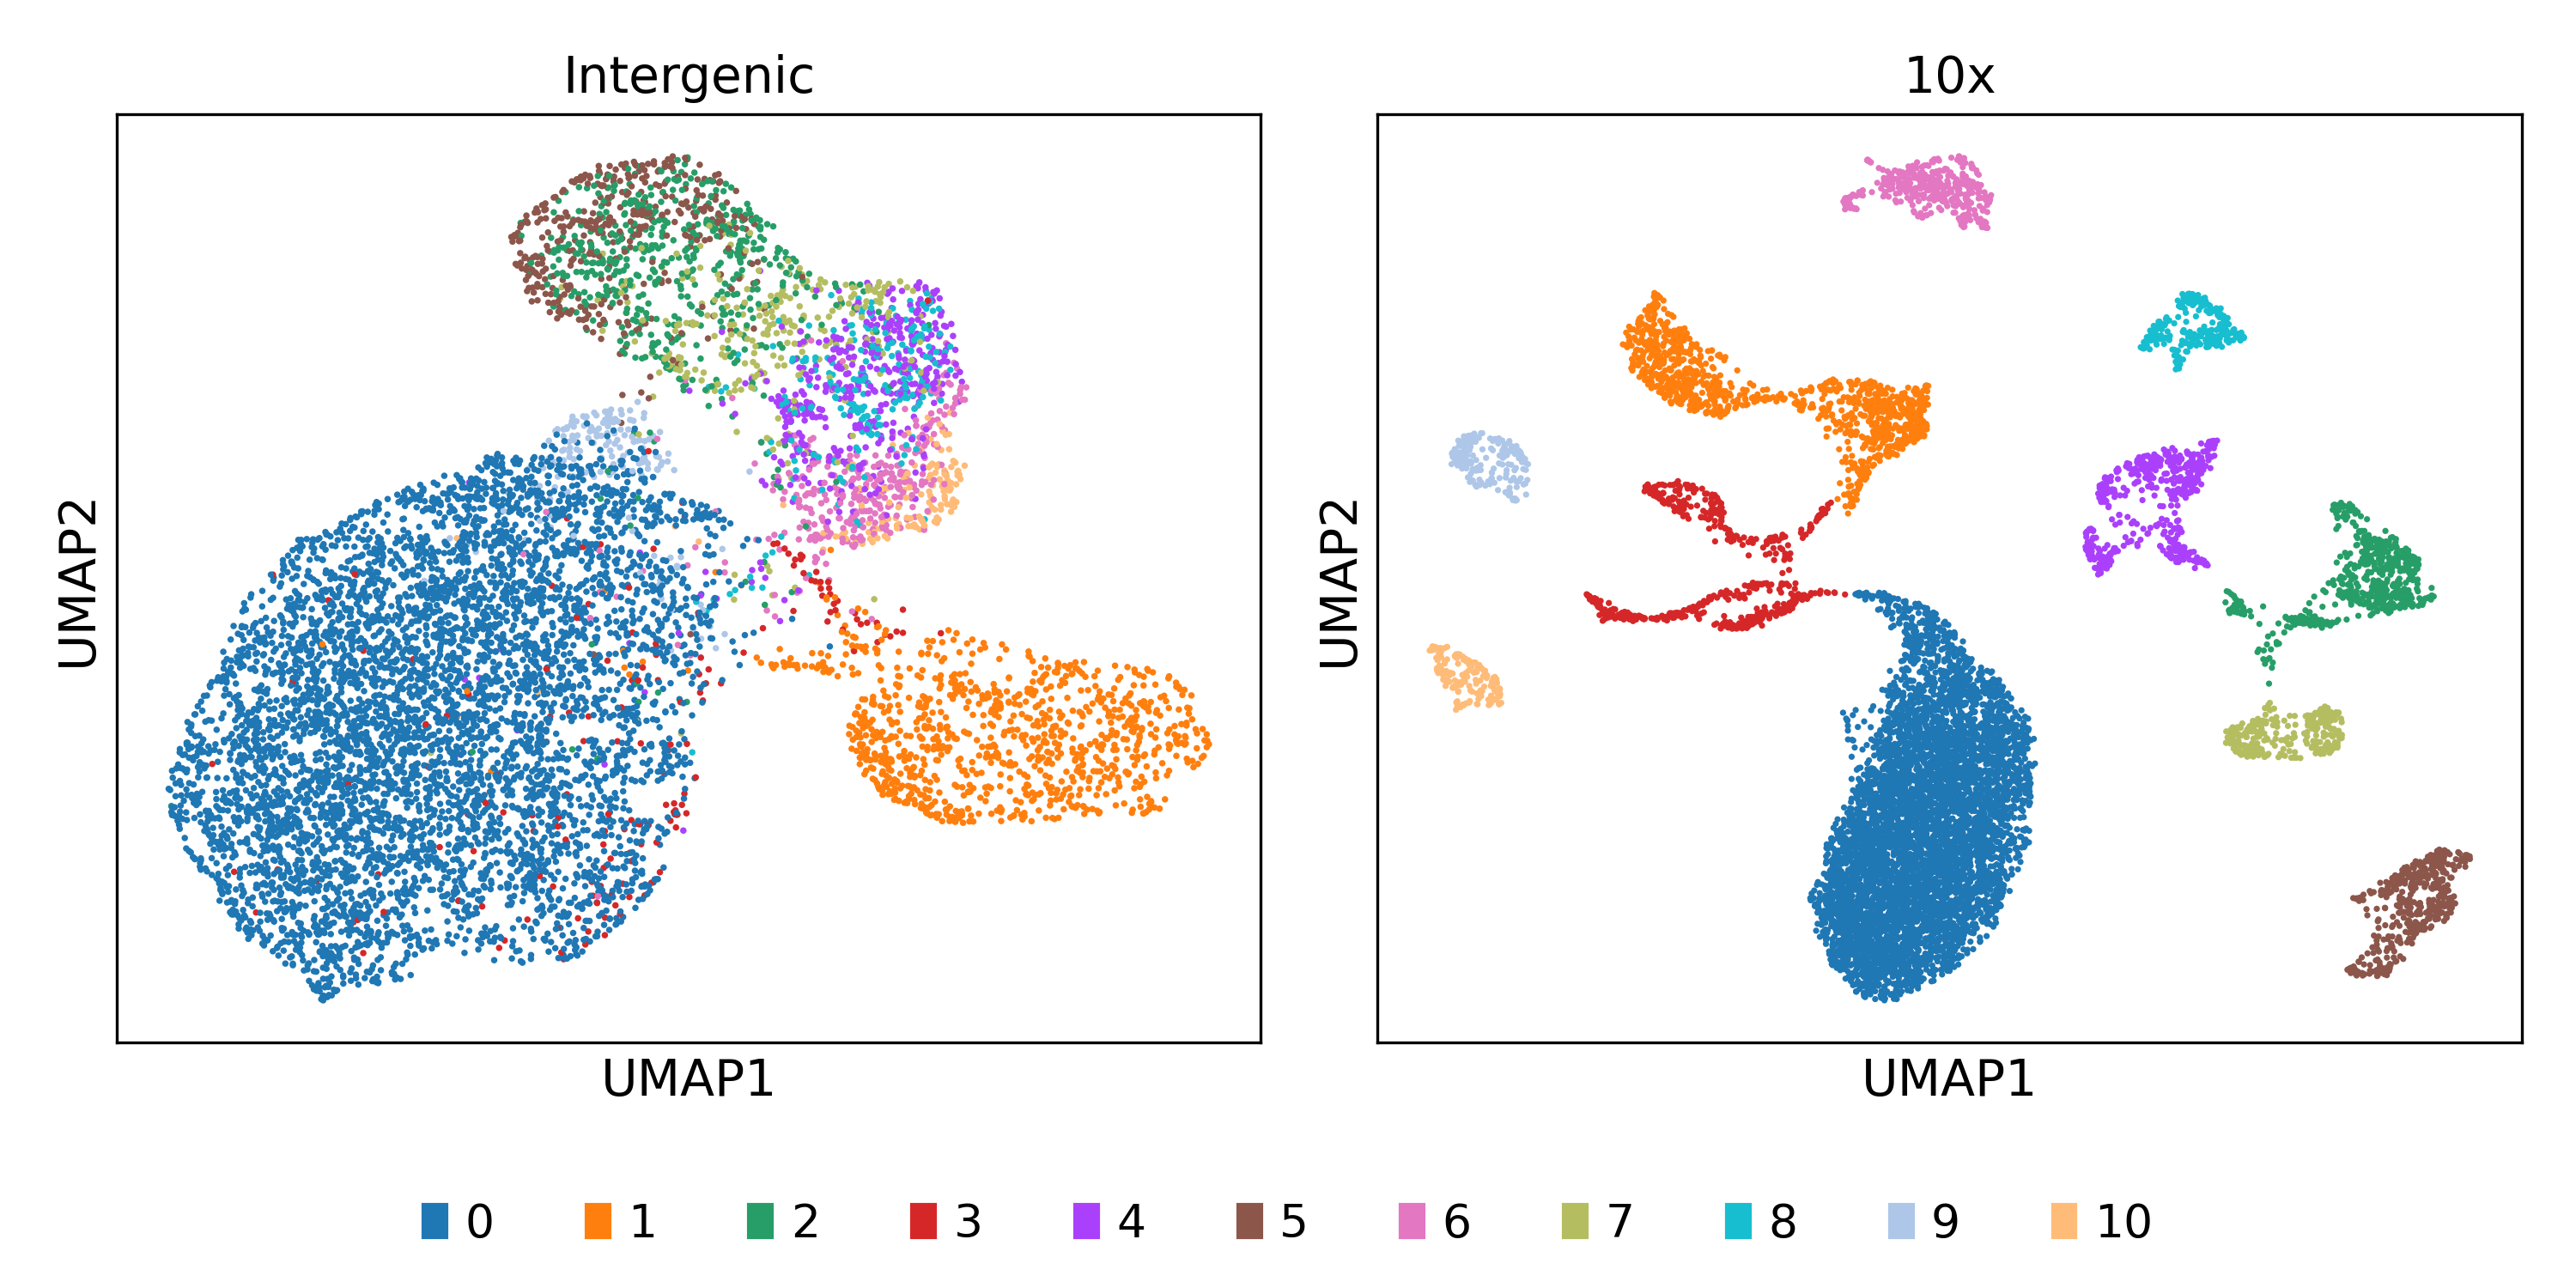
\includegraphics[width=\textwidth]{images/umaps/intergenic_10x_eye.png}
        \caption{eye}
    \end{subfigure}
    \hfill
    \begin{subfigure}{0.45\textwidth}
        \centering
        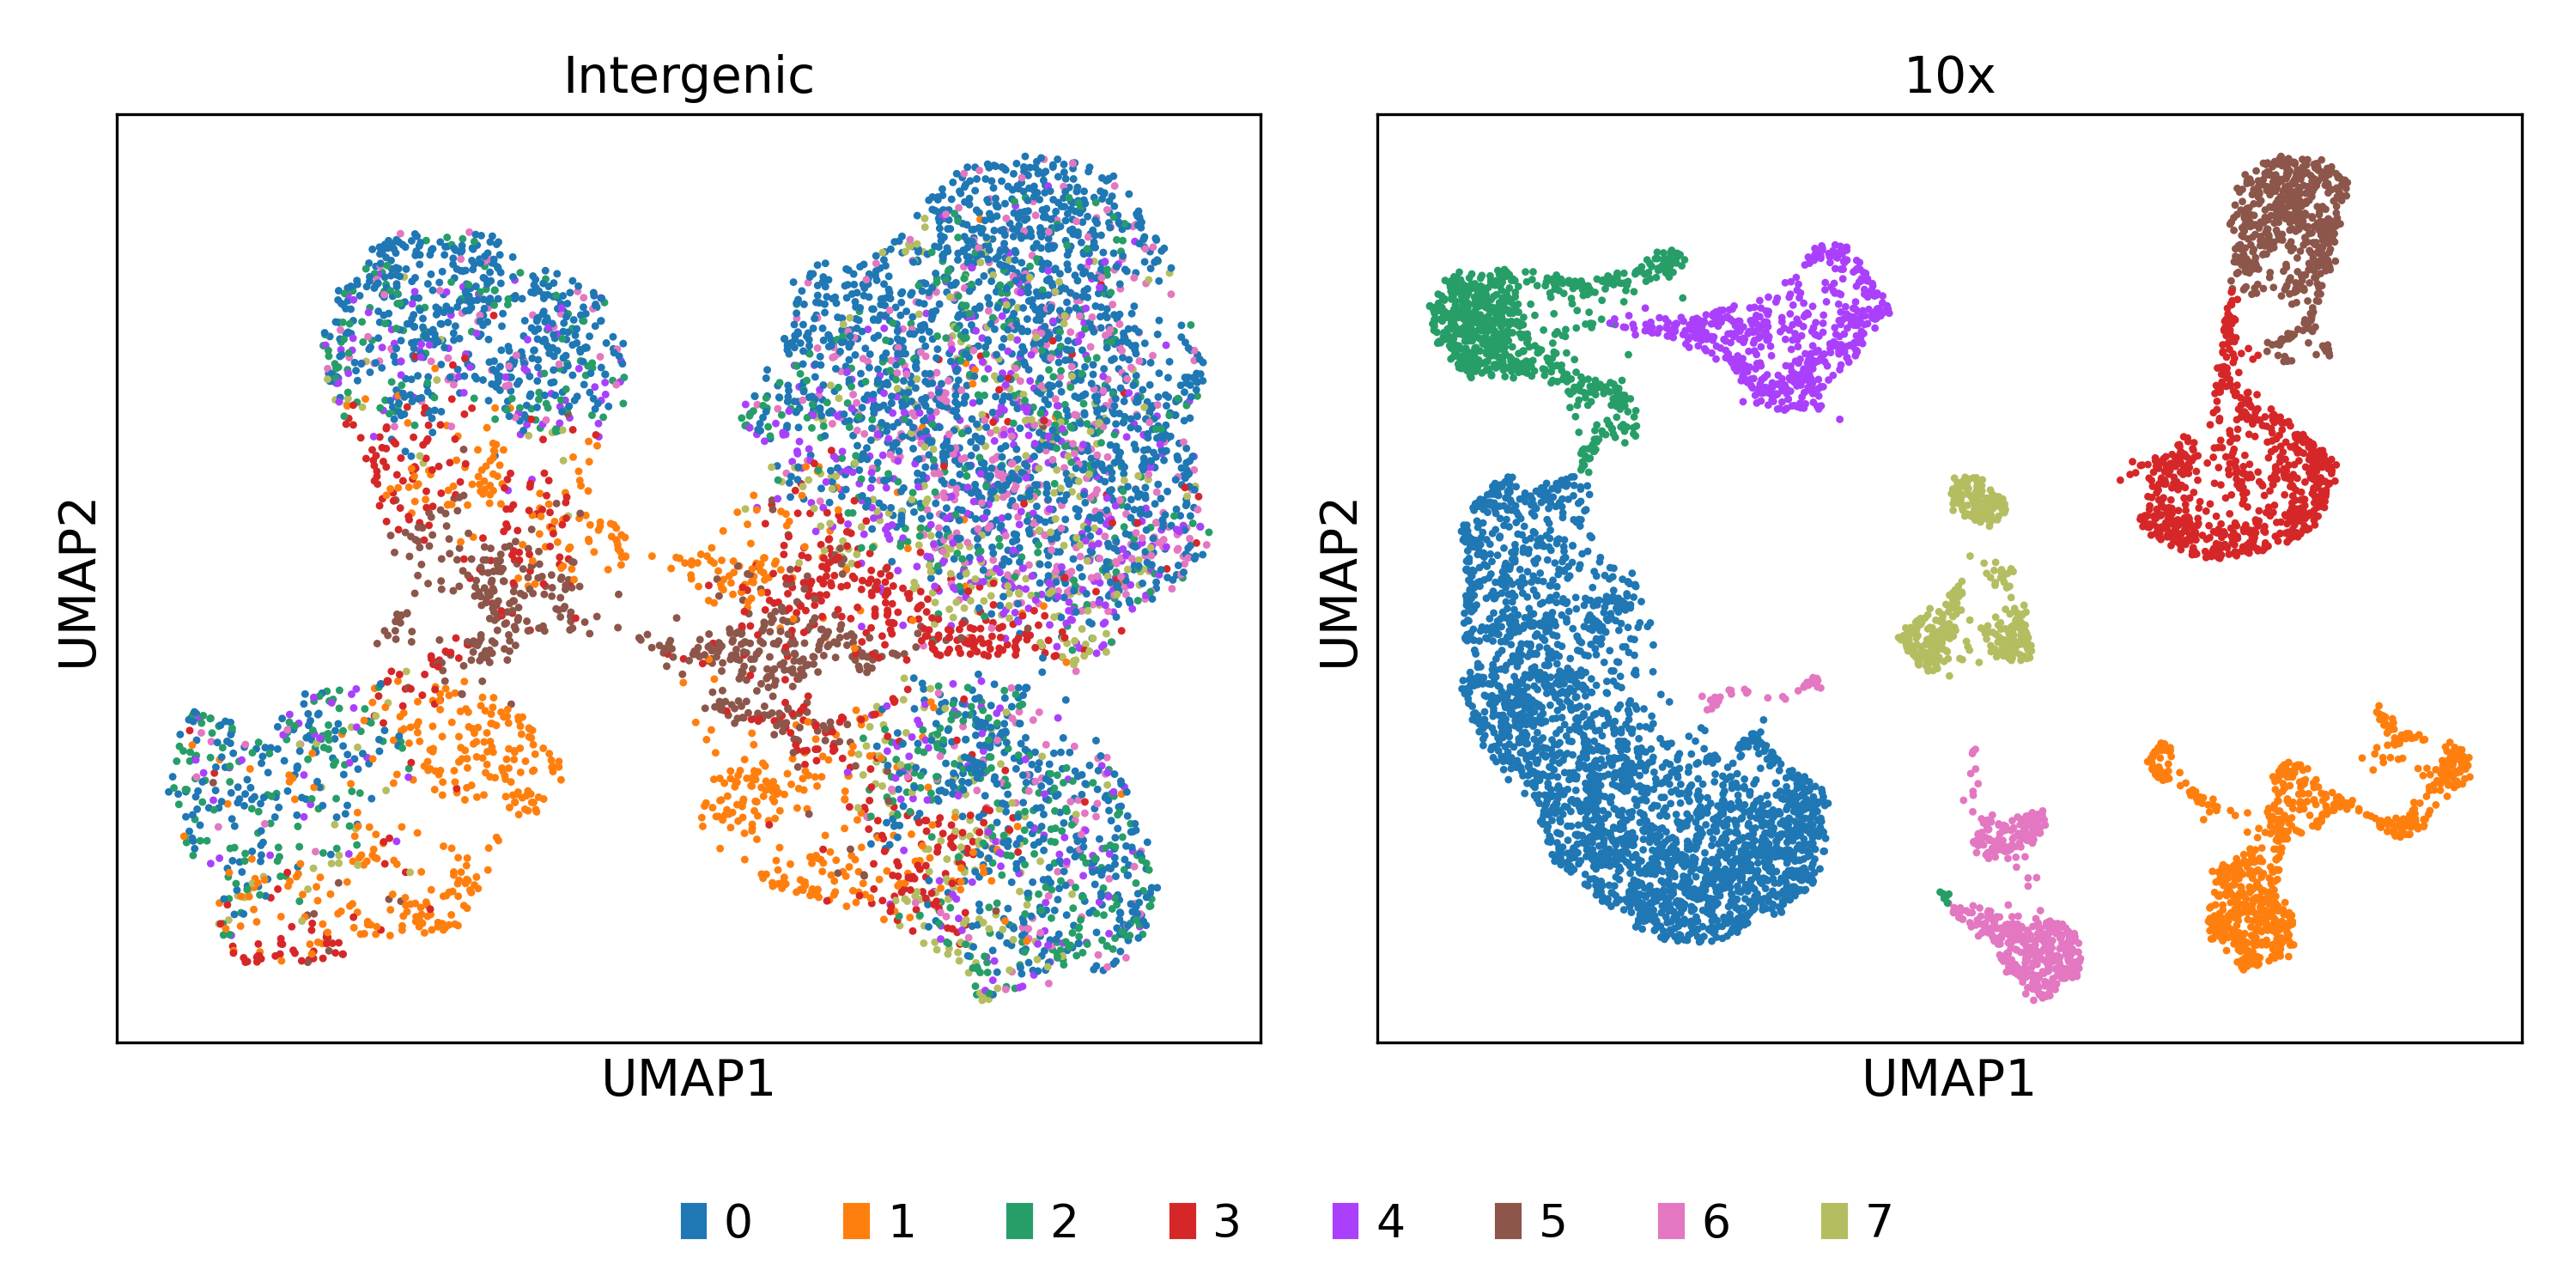
\includegraphics[width=\textwidth]{images/umaps/intergenic_10x_brain_2.png}
        \caption{10x Brain 2}
    \end{subfigure}
    \caption{Comparison of clustering using standard annotation ('10x' reference) and using only defined intergenic regions.
    As can be seen, for some samples intergenic regions are sufficient for rough clustering, for others (e.g. 'brain\_2' sample), 
    noise gives some clustering artefacts.
    Nevertheless, the clustering can be seen even in those noisy samples.}
    \label{fig:intergenicClustering}
\end{figure}

\subsection{Intergenic regions with high conservation score}

The filtering based on the conservation as described above left five intergenic regions, given in the Table \ref{tab:conservedIntergenic}.

\begin{table}[h]
    \centering
    \begin{tabular}{lccc}
        \toprule
        Name & Genomic coordinates & Conservation score & Found in samples \\
        \midrule
        INT1216 & 1:72282700-72282900 & 0.7534172617 & brain, eye\\
	INT1829 & 1:77772950-77773050 & 0.6863111111 & lung \\
	INT2199 & 6:148122550-148122750 & 0.6364459652 & brain, eye \\
	INT2208 & 5:18162950-18163100 & 0.6138651685 & PBMC (indrops) \\
	INT3636 & X:129412750-129413050 & 0.7218984354 & brain \\
        \bottomrule
    \end{tabular}
    \caption{Conserved intergenic regions not overlapping with known genes from ncbi and gencode annotations.}
    \label{tab:conservedIntergenic}
\end{table}

\subsection{Gene Predictions Tools}

61 intergenic regions overlap with predicted genes from UCSC gene prediction archive, given in the Table \ref{tab:predictionToolsIntergenic}.
Of them 44 are in the 3' end of predicted gene (good, as our datasets are generated using 3' end sequencing protocols).
Out of those 44 predicted genes, 15 are extended versions of genes present in gencode/ncbi references,
you can see an example in Figure \ref{fig:predictedExtention}.

\begin{figure}
  \centering
  \includegraphics[width=\linewidth]{images/igv/INT33.png}
  \caption{Example of gene which is predicted to have some longer transcripts than are present in the gencode and ncbi annotations.
  The intergenic region is located after the 3' end of gene DUSP1, however,
  SIB prediction tool suggest that longer transcripts should be included in the annotation of this gene.}
  \label{fig:predictedExtention}
\end{figure}


\begin{table}[h]
    \tiny
    \centering
    \begin{tabular}{lccc}
        \toprule
        Name & Genomic coordinates & Prediction tool & Overlaps with 3' region of predicted gene \\
        \midrule
	INT7 & 6:24718850-24719100 & SIB & Yes \\
	INT33 & 5:172767250-172767500 & SIB & Yes (DUSP1) \\
	INT134 & 15:41280550-41280800 & SIB & Yes (extends a bit after) \\
	INT196 & 6:89086200-89086500 & SIB & Yes (PNRC1) \\
	INT218 & 5:61409150-61409400 & SPG & No (5' end) \\
	INT285 & 10:110898200-110898550 & SIB & Yes (BBIP1) \\
	INT327 & 1:169132100-169132350 & SIB & Yes (NME7) \\
	INT347 & 14:75277700-75278000 & Gescan & No \\
	INT382 & 12:11892250-11892500 & Gescan & Yes \\
	INT386 & 6:26215200-26215450 & SIB & Yes (H2BCB?) \\
	INT438 & 4:39713300-39713600 & SIB & Yes (almost all (short) gene spanned) \\
	INT533 & 8:130110900-130111150 & SIB & Yes \\
	INT617 & 15:85733950-85734200 & SIB & Yes \\
	INT621 & 9:75148850-75149400 & SIB & Yes (OSTF1) \\
	INT651 & 1:28579100-28579350 & SIB & Yes (TRNAU1AP) \\
	INT654 & 6:34382850-34383050 & SIB & No (but short gene)\\
	INT827 & 9:94111950-94112200 & SIB & Yes \\
	INT828 & 8:133035800-133036050 & SIB & Yes (SLA) \\
	INT859 & 2:71373500-71373750 & SIB & No (slight overlap on 5' end) \\
	INT898 & 17:51190400-51190700 & SIB & Yes (extends after)\\
	INT903 & 8:22613400-22613650 & SIB & Yes \\
	INT949 & 9:111693050-111693400 & SIB & Yes \\
	INT972 & 15:64954800-64955350 & SIB & Yes \\
	INT984 & 18:63291900-63292200 & Geneid & Yes No \\
	INT1028 & 5:50414200-50414500 & SIB & Yes No \\
	INT1155 & 1:36296050-36296300 & SIB & Yes No \\
	INT1216 & 1:72282700-72282900 & SIB & Yes No \\
	INT1231 & 10:19890700-19891050 & Gescan & Yes No \\
	INT1387 & 11:63570800-63571050 & SIB & Yes No \\
	INT1402 & 5:142786700-142786950 & SIB & Yes No \\
	INT1440 & 2:235746450-235746700 & SIB & Yes No \\
	INT1445 & 9:40885650-40885900 & SIB & Yes No \\
	INT1525 & 8:11842200-11842350 & SIB & Yes No \\
	INT1548 & 7:50342700-50342950 & Gescan & Yes No \\
	INT1616 & 17:30895450-30895700 & SIB & Yes No \\
	INT1749 & 3:172333550-172333750 & SIB & Yes No \\
	INT1801 & 5:151272550-151272700 & SIB & Yes No \\
	INT1931 & 17:82522100-82522350 & SIB & Yes No \\
	INT2044 & 19:4041150-4041400 & SIB & Yes No \\
	INT2065 & 10:103606150-103606400 & SIB & Yes No \\
	INT2158 & 14:49636100-49636350 & SIB & Yes No \\
	INT2194 & 7:130521250-130521500 & SIB & Yes No \\
	INT2371 & 1:14632650-14632900 & Geneid & Yes No \\
	INT2380 & 22:33853900-33854150 & Geneid & Yes No \\
	INT2825 & 13:45300050-45300300 & Geneid & Yes No \\
	INT2979 & 4:98929350-98929600 & SIB & Yes No \\
	INT3328 & 2:184604250-184604500 & SIB & Yes No \\
	INT3429 & 17:48172750-48173150 & Augustus & Yes No \\
	INT3504 & 15:25332950-25333150 & SIB & Yes No \\
	INT3849 & 3:121432200-121432400 & SIB & Yes No \\
	INT3868 & 17:31448500-31448700 & SIB & Yes No \\
	INT4070 & 4:47430500-47430700 & SIB & Yes No \\
	INT4147 & 1:34861500-34861700 & SIB & Yes No \\
	INT4458 & 5:44820700-44820900 & SIB & Yes No \\
	INT4577 & 5:702050-702300 & SIB & Yes No \\
	INT4743 & 20:3188900-3189050 & SIB & Yes No \\
	INT4948 & 5:703250-703450 & SIB & Yes No \\
	INT5002 & 11:92232750-92232950 & SIB & Yes No \\
	INT5315 & 20:3183750-3184050 & SIB & Yes No \\
	INT5329 & 13:95603000-95603200 & SIB & Yes No \\
	INT5710 & 4:47428500-47428700 & SIB & Yes No \\
        \bottomrule
    \end{tabular}
    \caption{Intergenic regions overlapping with predicted genes from UCSC gene prediction archive.}
    \label{tab:predictionToolsIntergenic}
\end{table}


\subsection{Intergenic regions specific to some cell types}

If reads from specific intergenic region are specific for only subset of cell types present in the sample,
it is strong indication that those reads are not sequencing artefacts.
Examples of such regions can be seen in the Figure \ref{fig:intergenicSpecific}.

\begin{figure}[htbp]
    \centering
    \begin{subfigure}{0.45\textwidth}
        \centering
        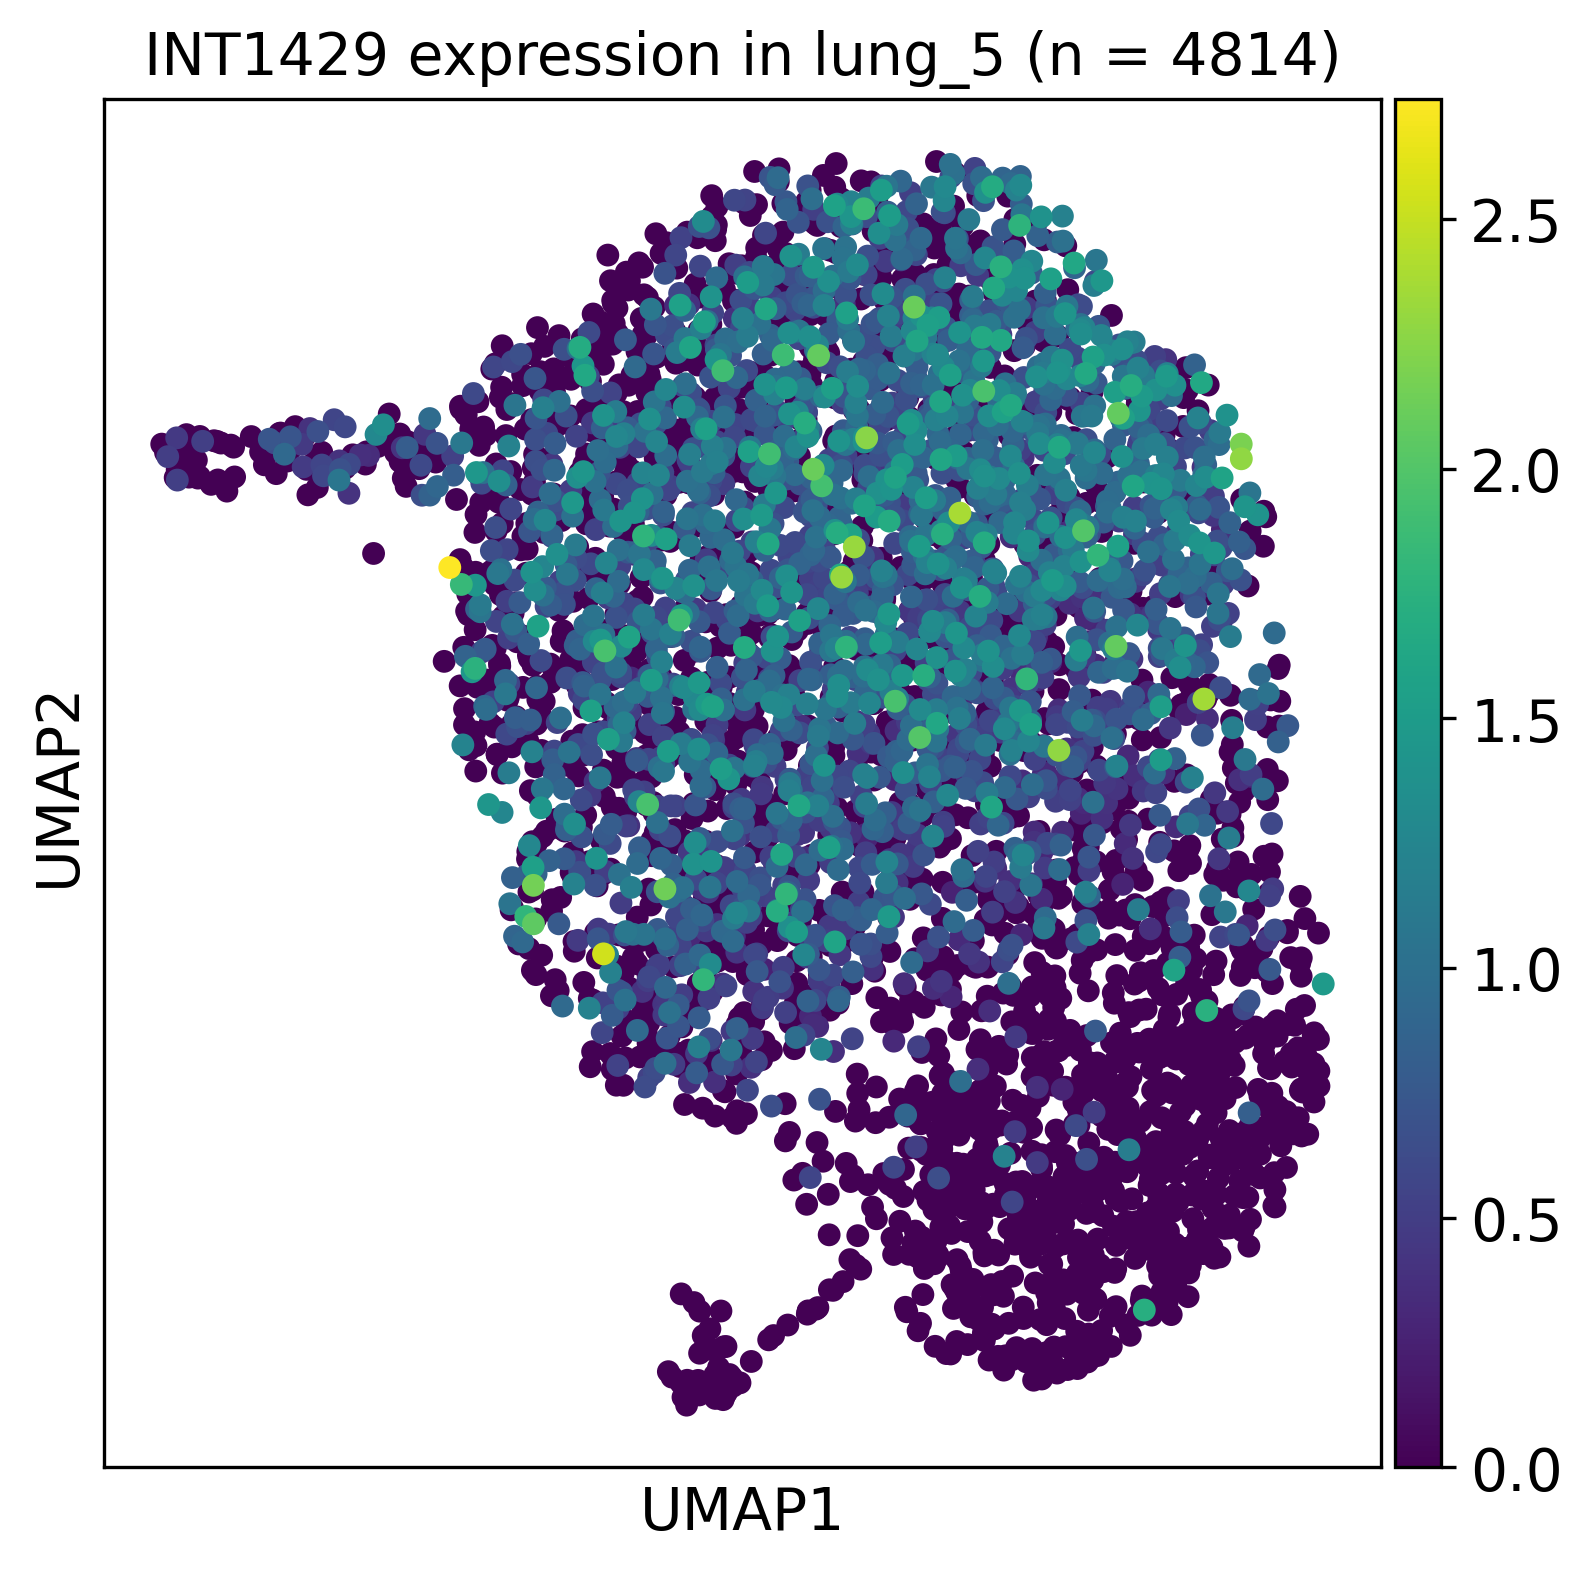
\includegraphics[width=\textwidth]{images/intergenicSpecificExamples/INT1429_lung_5.png}
        \caption{Lung 5 (INT1429)}
    \end{subfigure}
    \hfill
    \begin{subfigure}{0.45\textwidth}
        \centering
        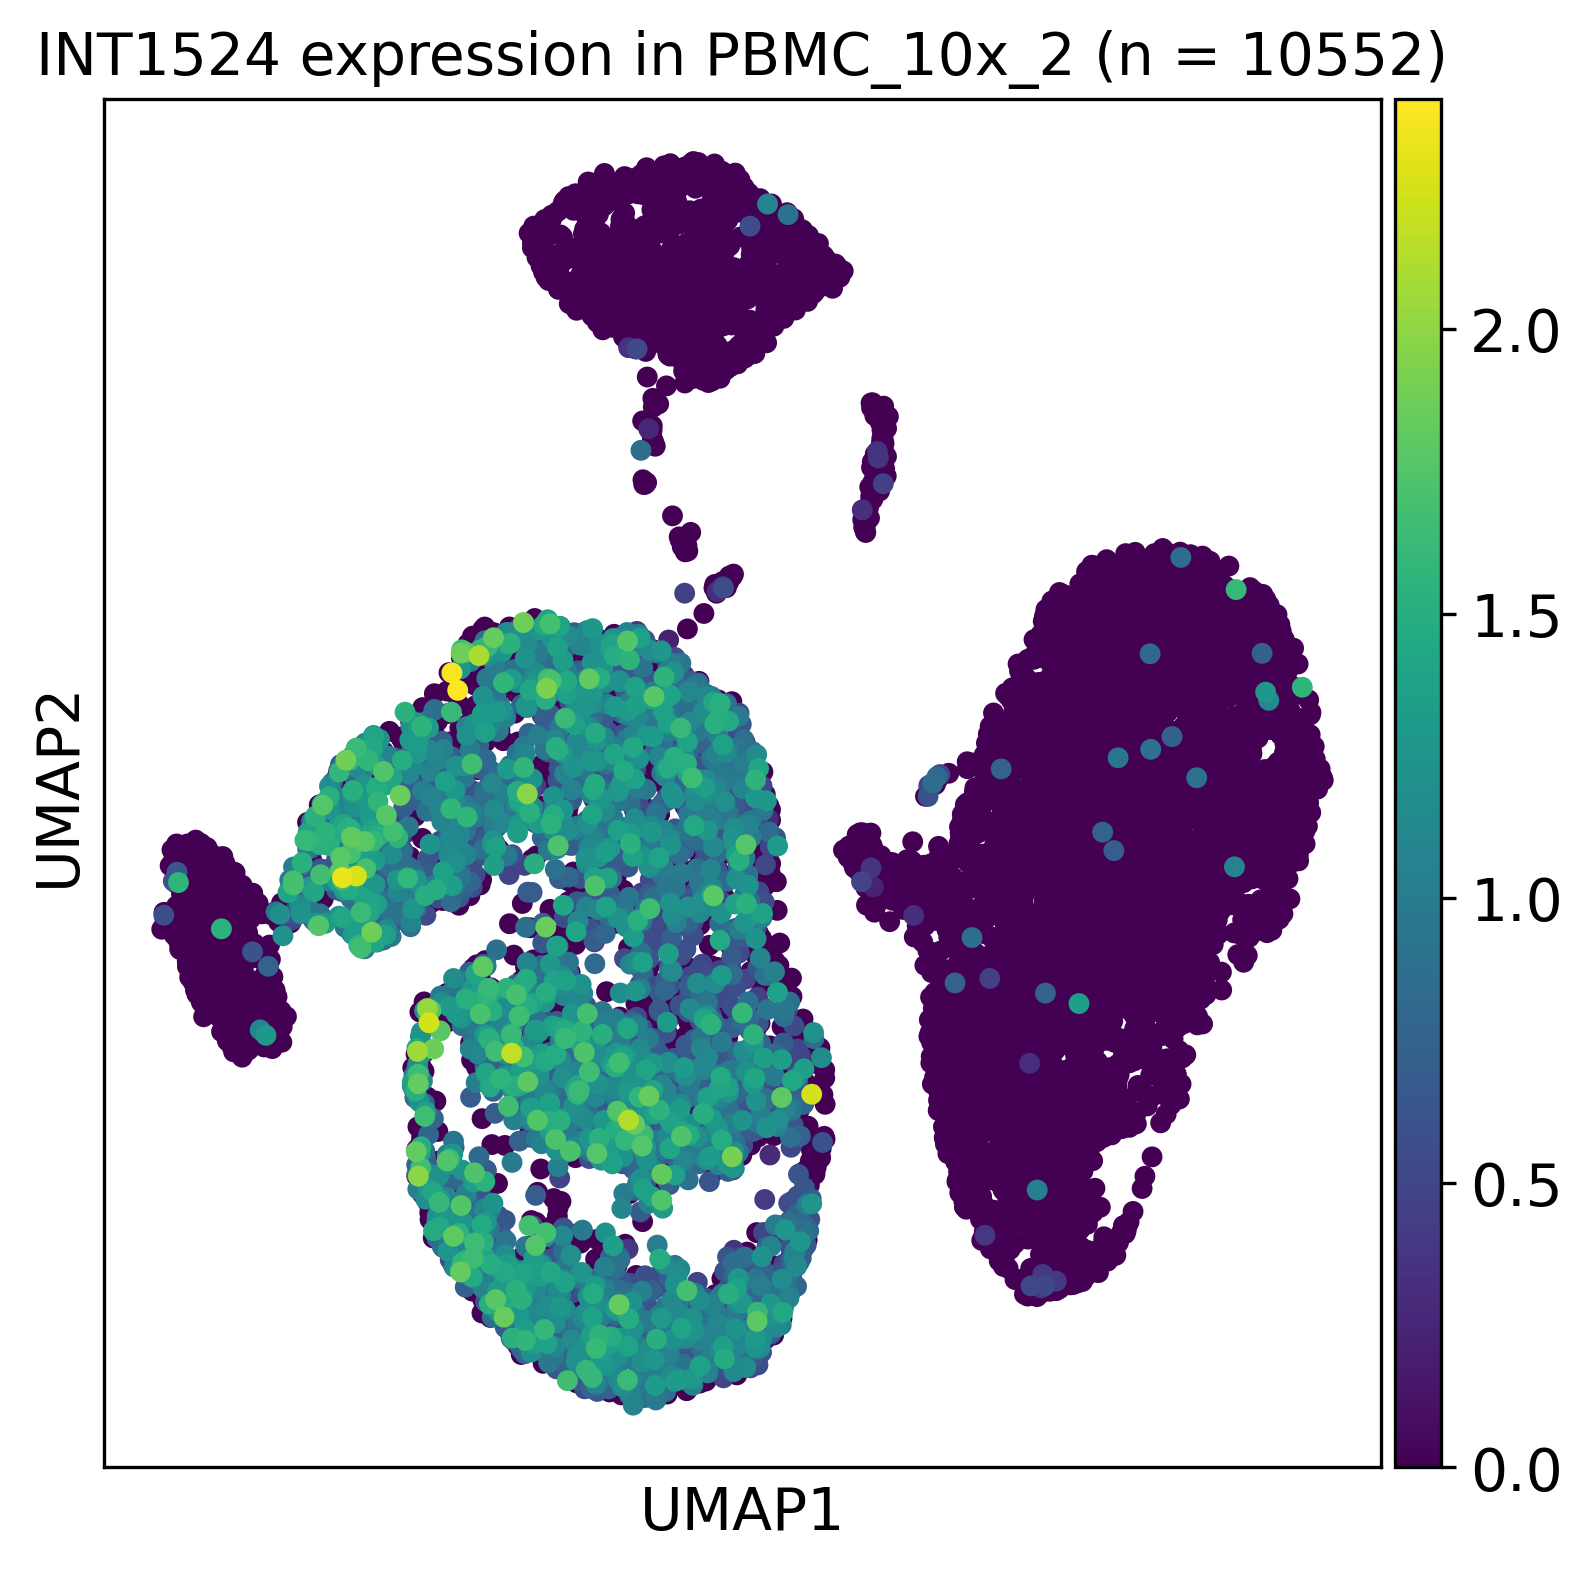
\includegraphics[width=\textwidth]{images/intergenicSpecificExamples/INT1524_PBMC_10x_2.png}
        \caption{PBMC 10x 2 (INT1524)}
    \end{subfigure}
    \vspace{0.5em}
    \begin{subfigure}{0.45\textwidth}
        \centering
        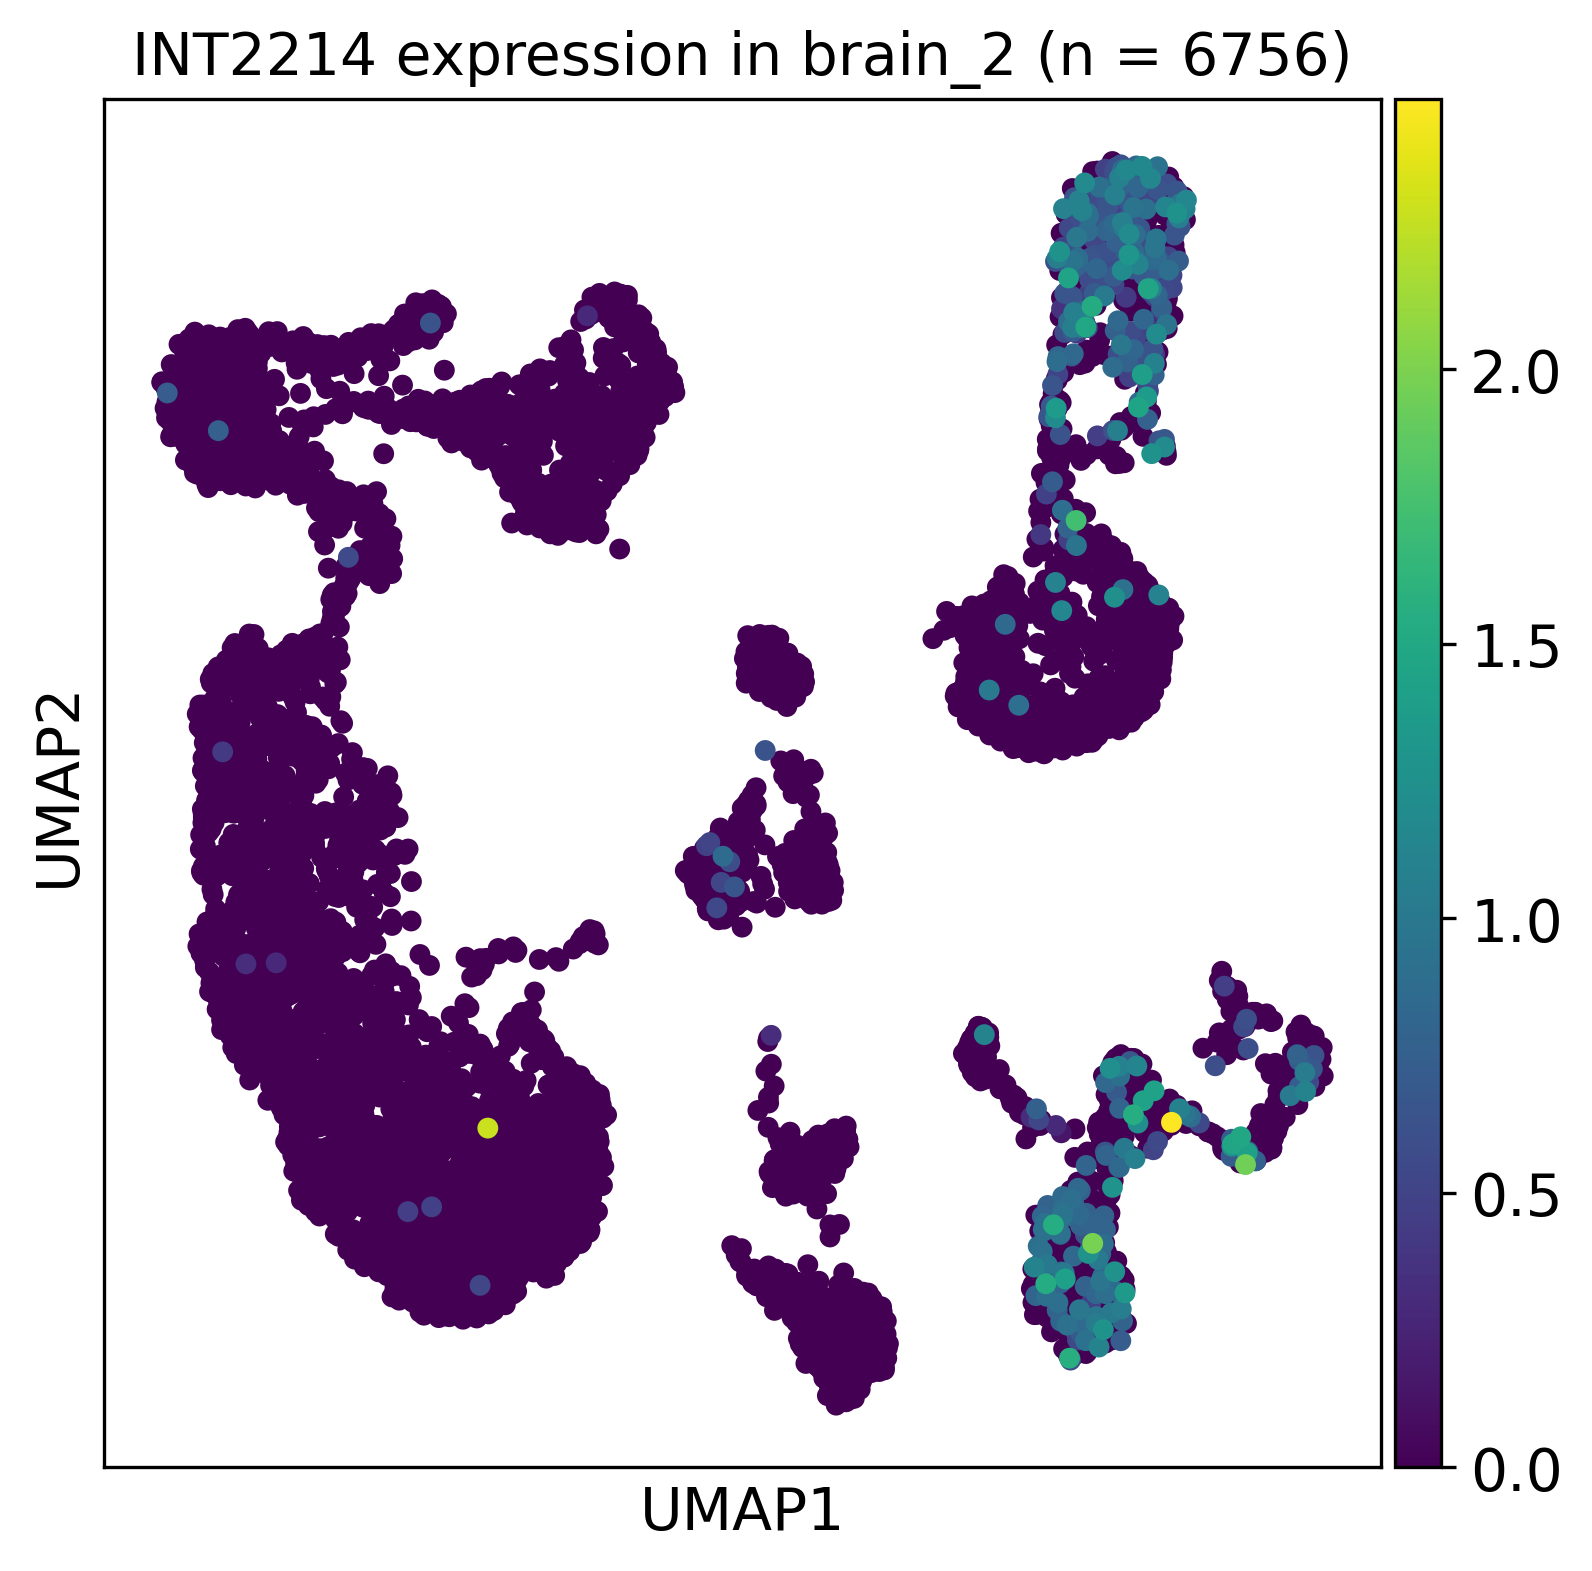
\includegraphics[width=\textwidth]{images/intergenicSpecificExamples/INT2214_brain_2.png}
        \caption{Brain 2 (INT2214)}
    \end{subfigure}
    \hfill
    \begin{subfigure}{0.45\textwidth}
        \centering
        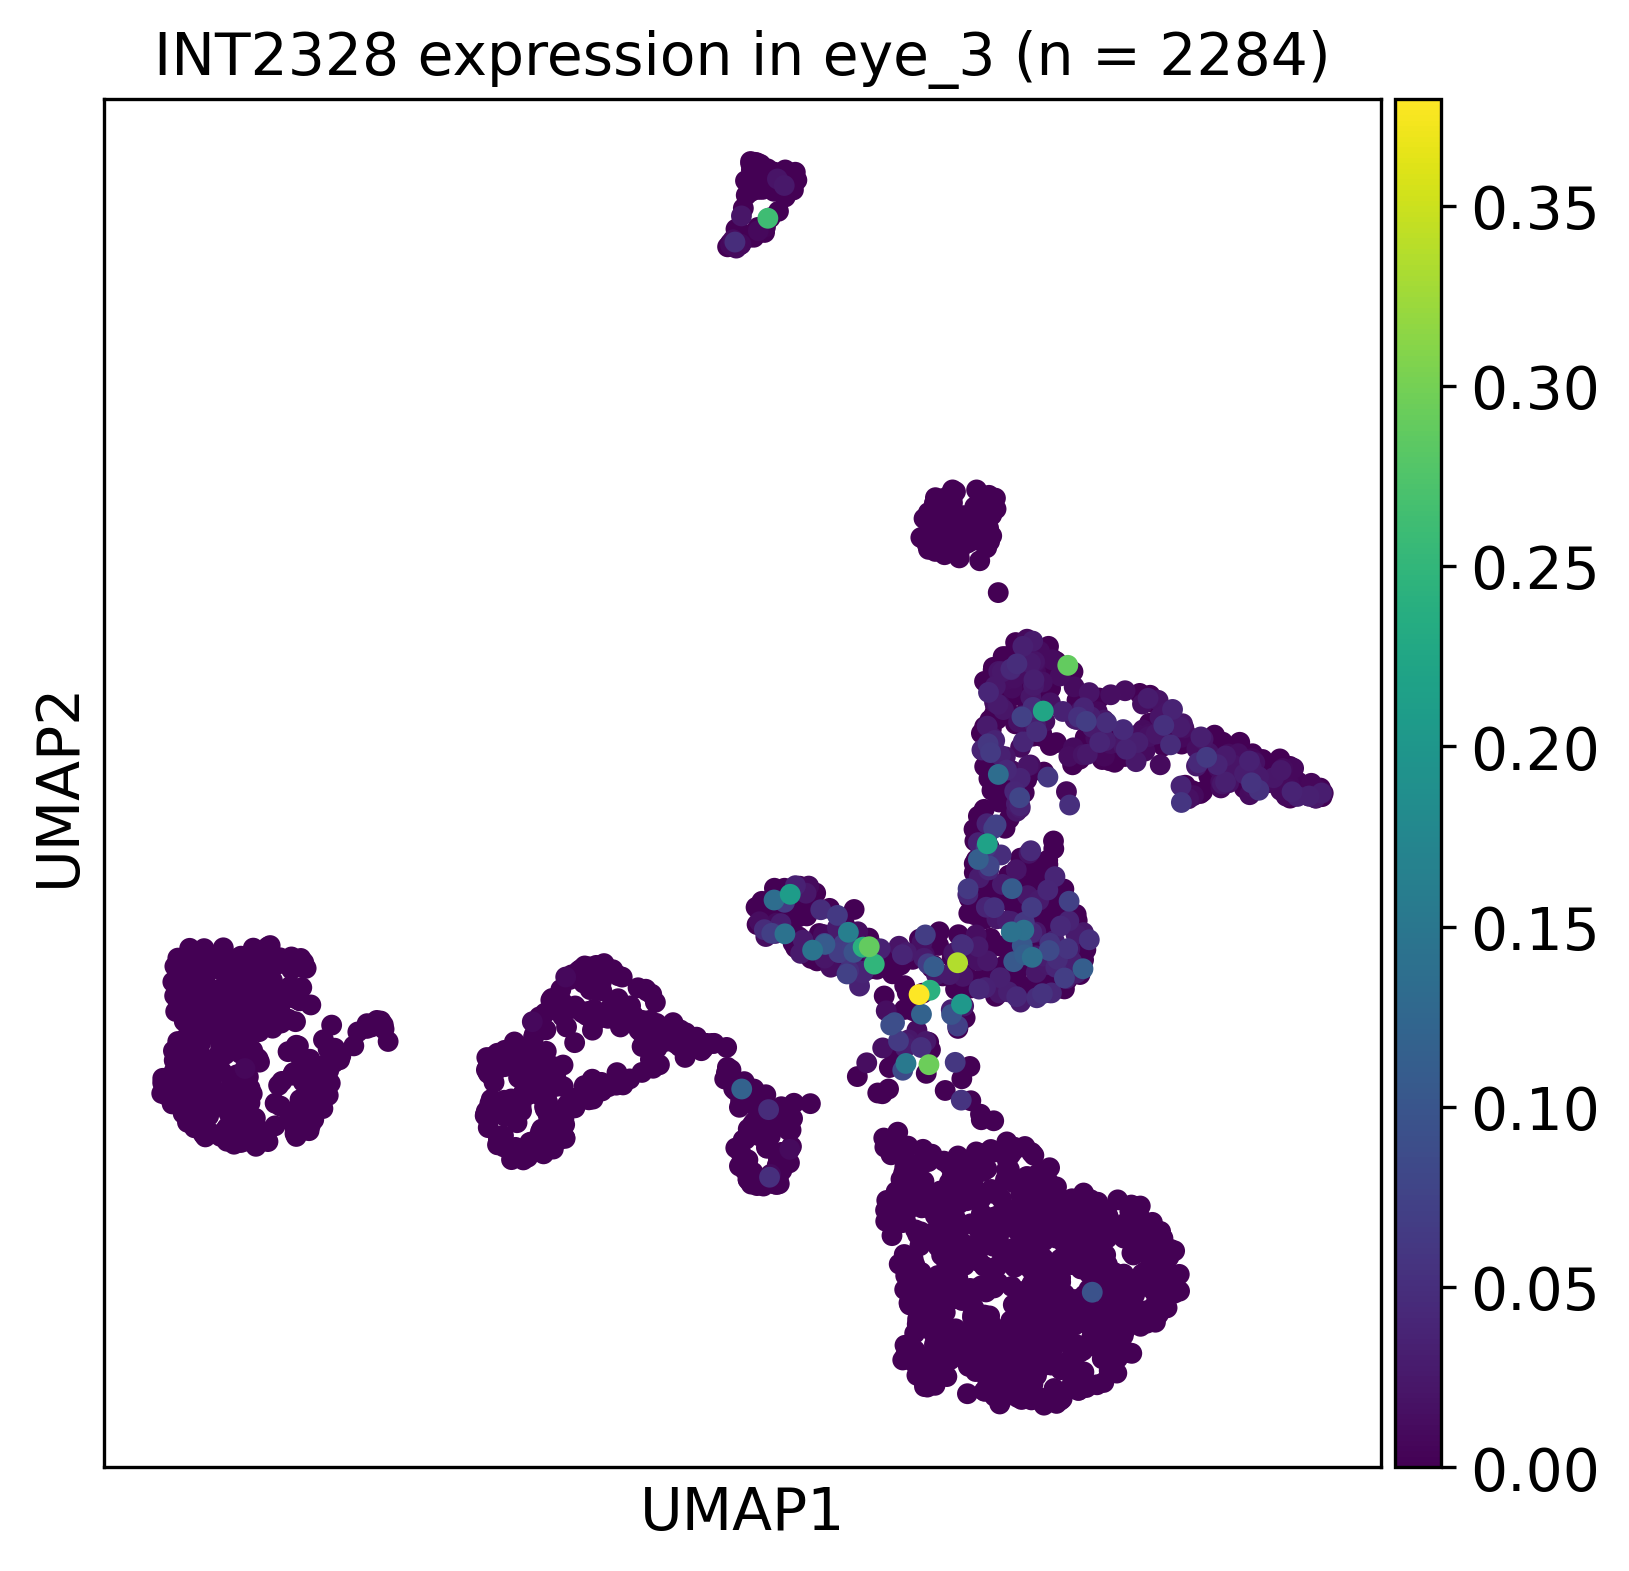
\includegraphics[width=\textwidth]{images/intergenicSpecificExamples/INT2328_eye_3.png}
        \caption{Eye 3 (INT2328)}
    \end{subfigure}
    \caption{Some examples of specificly expressed intergenic regions in various samples.}
    \label{fig:intergenicSpecific}
\end{figure}

\subsection{ATAC data}

ATAC sequencing shows open chromatin sites, which could potentially indicate that some transcription activity is happening at those sites.
Hence, checking if there are overlaps between open chromatine regions and dewfined intergenic regions could provide additional evidence of
those regions being not noise.
However, there are some caveats in this 'evidence'.
Firstly, open chromatin is mostly expected at the transcription start sites, promoter or other regulatory elements,
which are typically located in the 5' end of the gene.
Another problem is that majority of our defined regions lay on the opposite strands of known genes, while ATAC sequencing is not strand specific.
In such cases, open chromatine could be present due to the transcription of those known genes.

Out of 2590 intergenic regions, 309 intersected with ATAC intervals found from 10x PBMC ATAC data.
Out of those 309 regions, only 20 were not overlapping with genes from GENCODE or RefSeq annotations.

\subsection{Correlations}

Another aspect to check is whether expression of those intergenic regions correlate with the expression of nearby genes.
If it does, it might indicate several things:
\begin{itemize}
  \item If the region correlates with gene on the same strand:
  \begin{itemize}
    \item There might exist longer unannotated transcripts that involve those intergenic regions.
    \item The intergenic genes are involved in the same processes as the gene.
    \item They both can be transcribed by the same polymerases.
  \end{itemize}
  \item If the region correlates with gene on the oposite strand:
  \begin{itemize}
    \item The intergenic gene is involved in the same processes as the gene on the oposite strand.
    \item There happens some transcription errors that cause transcription from the opposite strand.
    \item There happens some errors in the library preparation/sequencing steps that cause template switch.
  \end{itemize}
\end{itemize}

Which of those are the case in our samples, is hard to tell.
Out of all defined intergenic regions, 86 showed Spearman correlation \textgreater 0.5 (p \textless 0.05) in at least 1 sample
(80 correlated with genes on the opposite strand, 10 with gene on the same strand, 4 with both).
Some examples can be seen in Figure \ref{fig:correlationUmaps}.

\begin{figure}[htbp]
    \centering
    \begin{subfigure}{\textwidth}
        \centering
        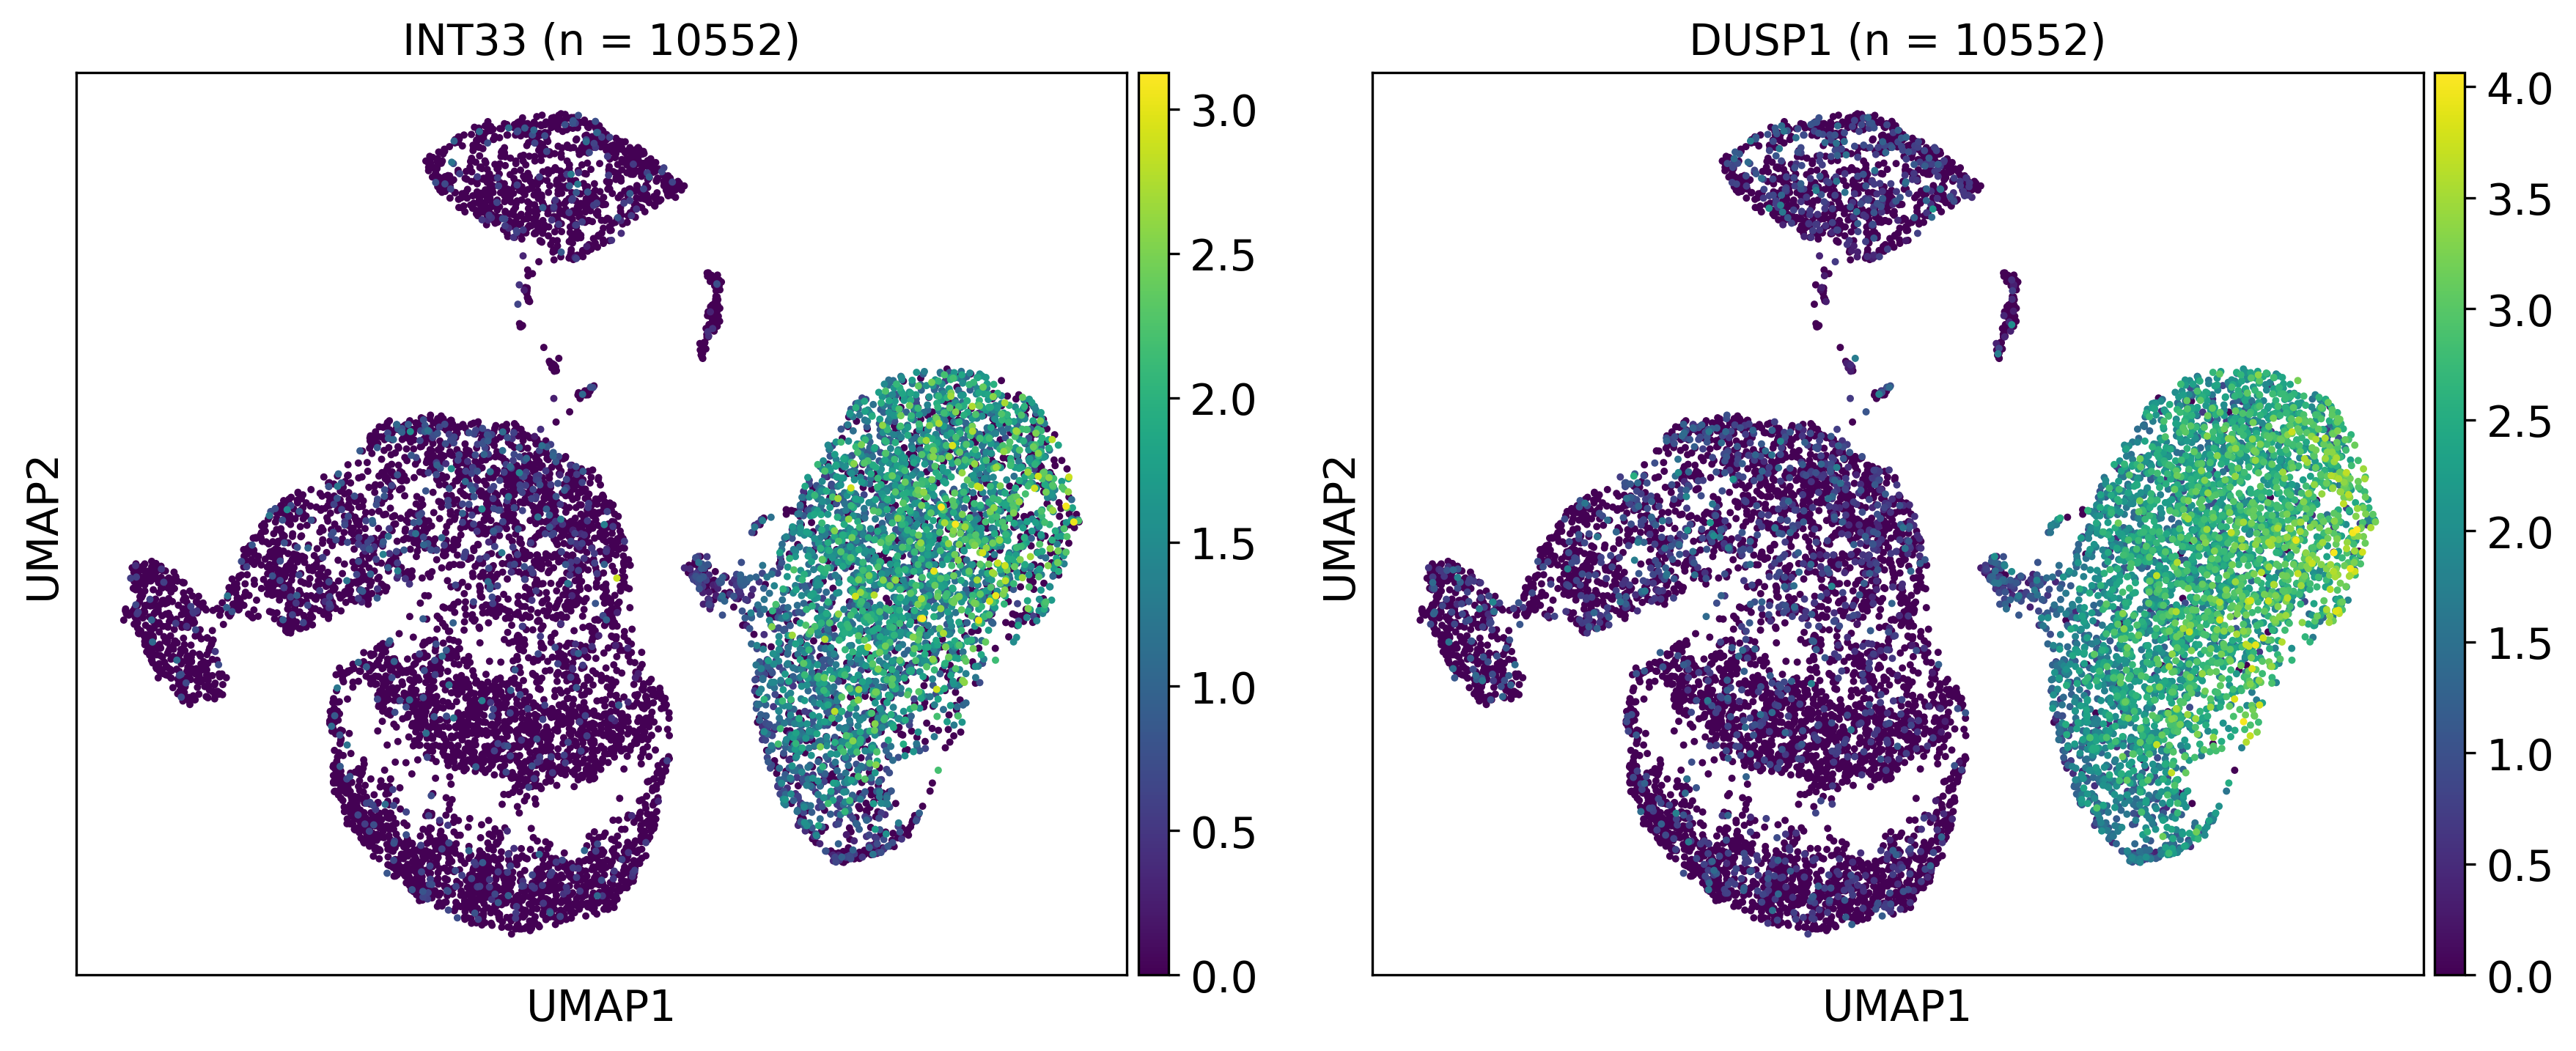
\includegraphics[width=\textwidth]{images/correlationUmaps/PBMC_10x_2_DUSP1.png}
        \caption{Umaps of INT33 and DUSP1 (Spearman correlation 0.68) of the PBMC\_10x\_2 sample, both of them are on the same strand.}
    \end{subfigure}
    \vspace{0.5em}
    \begin{subfigure}{\textwidth}
        \centering
        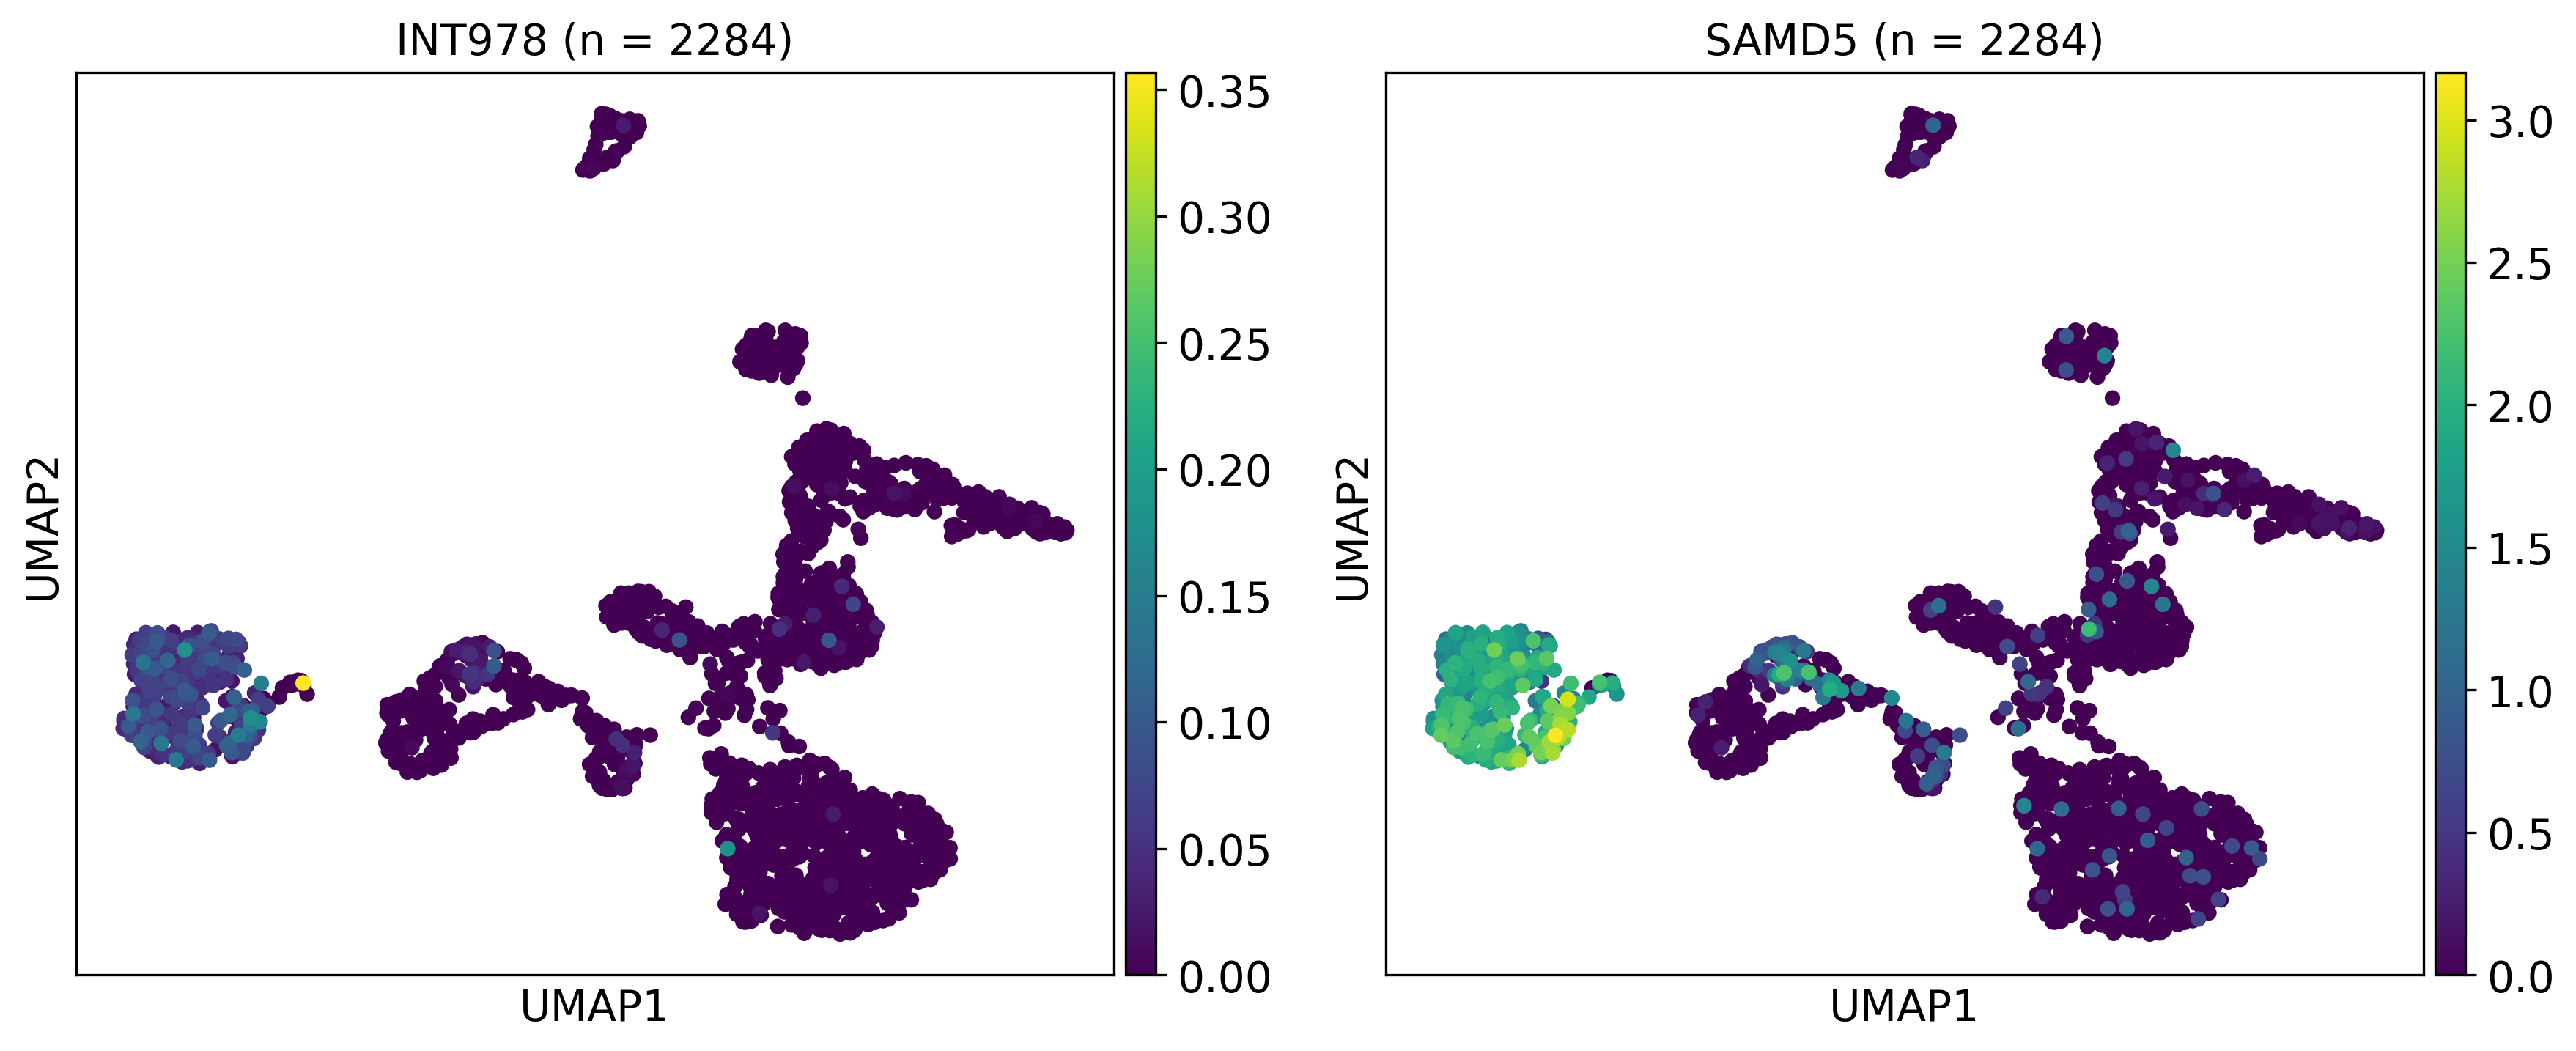
\includegraphics[width=\textwidth]{images/correlationUmaps/eye_3_SAMD5.png}
        \caption{Umaps of INT978 and SAMD5 (Spearman correlation 0.85) of the eye\_3 sample,
        intergenic region is on the opposite strand of the gene.}
    \end{subfigure}
    \caption{Correlation can be seen visually in UMAPs (colored by the normalized expression of the genes), here couple of examples given.}
    \label{fig:correlationUmaps}
\end{figure}

\fi



\iffalse

\section{Enhancing transcriptomic reference}

The enhanced transcriptomic reference allows to include those reads into downstream analysis that otherwise would be discarded.
To achieve this, we have combine data from several different transcriptomic annotations,
and additionally included in the annotation intergenic regions that contained relativelly high number of reads.

\input{"data/downstream/summaries/count_summaries/count_summary.tex"}

\subsection{Exploring unassigned reads}
Unassigned reads could come from several sources:
sequencing artefacts, genes that are not included into transcriptomic reference used, or genes that are not annotated yet.
To check, we have looked at intersections of those unassigned reads and more comprehensive annotations.
As we can see, that there are plenty of genes from more comprehensive annotations which intersect with unassigned genes,
and number of those intersecting genes correlates with sequencing depth.

\input{"data/downstream/summaries/gene_summaries/intersecting_gene_summary.tex"}

\subsection{Intergenic regions}

Observed intergenic regions can be either artefacts or be biologically meaningfull.
To check this, I have tried to cluster cells based only on the newly defined intergenic regions (see figure \ref{fig:umapComparisonIntergenic}).
While for PBMC\_indrops sample it looks as noise, for the 10x indrops samples it provides quite good clustering,
meaning that at least some of those captured intergenic regions are not sequencing artefacts.

\subsection{Enhanced Reference}

Using enhanced reference allowed us to have more captured genes in the data,
however, no significant change in clustering can be seen.

\input{"data/downstream/summaries/captured_gene_summaries/captured_gene_types_summary.tex"}

\subsection{Captured genes}

\fi
